\documentclass[12pt, a4paper]{report}
\usepackage[english]{babel}
\usepackage[utf8]{inputenc}
\usepackage[T1]{fontenc}
\usepackage[protrusion=true,expansion,tracking=true,kerning=true]{microtype}
\usepackage{amsmath,amssymb}
\usepackage{lmodern}
\usepackage{bm}
\usepackage{accents}
\usepackage{mathrsfs}
\usepackage[hidelinks]{hyperref}
\usepackage{nameref}
\usepackage{parskip}
% \usepackage{xcolor}
\usepackage{graphicx}
% \usepackage[none]{hyphenat}
\usepackage{subcaption}
\usepackage{derivative}
\usepackage{enumerate}
\usepackage{enumitem}
\usepackage{array}
\usepackage{booktabs}
\usepackage{siunitx}
\usepackage[format=hang,position=bottom]{caption}
\usepackage[bottom]{footmisc}
\usepackage[backend=biber, style=numeric, sortcites=true]{biblatex}
\addbibresource{reference.bib}
\usepackage[capitalize]{cleveref}
\usepackage{csquotes}
\usepackage{lipsum}
\usepackage{tikz}
\usepackage{listings}

% Macros
\newcommand{\Ftot}{\mathbf{F}}
\newcommand{\iF}{\mathbf{F}^{-1}}
\newcommand{\tF}{\mathbf{F}^{T}}
\newcommand{\itF}{\mathbf{F}^{-T}}

\newcommand{\Fi}{\mathbf{F}_{i}}
\newcommand{\iFi}{\mathbf{F}_{i}^{-1}}
\newcommand{\tFi}{\mathbf{F}_{i}^{T}}
\newcommand{\itFi}{\mathbf{F}_{i}^{-T}}

\newcommand{\Fe}{\mathbf{F}_{e}}
\newcommand{\iFe}{\mathbf{F}_{e}^{-1}}
\newcommand{\tFe}{\mathbf{F}_{e}^{T}}
\newcommand{\itFe}{\mathbf{F}_{e}^{-T}}

\newcommand{\Ctot}{\mathbf{C}}
\newcommand{\iC}{\mathbf{C}^{-1}}
\newcommand{\tC}{\mathbf{C}^{T}}
\newcommand{\itC}{\mathbf{C}^{-T}}

\newcommand{\Etot}{\mathbf{E}}
\newcommand{\iE}{\mathbf{E}^{-1}}
\newcommand{\tE}{\mathbf{E}^{T}}
\newcommand{\itE}{\mathbf{E}^{-T}}

\newcommand{\Ci}{\mathbf{C}_{i}}
\newcommand{\iCi}{\mathbf{C}_{i}^{-1}}
\newcommand{\tCi}{\mathbf{C}_{i}^{T}}
\newcommand{\itCi}{\mathbf{C}_{i}^{-T}}

\newcommand{\Ce}{\mathbf{C}_{e}}
\newcommand{\iCe}{\mathbf{C}_{e}^{-1}}
\newcommand{\tCe}{\mathbf{C}_{e}^{T}}
\newcommand{\itCe}{\mathbf{C}_{e}^{-T}}

\newcommand{\btot}{\mathbf{b}}
\newcommand{\bbar}{\mathbf{\overline{b}}}
\newcommand{\ib}{\mathbf{b}^{-1}}
\newcommand{\tb}{\mathbf{b}^{T}}
\newcommand{\itb}{\mathbf{b}^{-T}}

\newcommand{\bi}{\mathbf{b}_{i}}
\newcommand{\ibi}{\mathbf{b}_{i}^{-1}}
\newcommand{\tbi}{\mathbf{b}_{i}^{T}}
\newcommand{\itbi}{\mathbf{b}_{i}^{-T}}


\newcommand{\be}{\mathbf{b}_{e}}
\newcommand{\bebar}{\mathbf{\overline{b}}_{e}}
\newcommand{\ibe}{\mathbf{b}_{e}^{-1}}
\newcommand{\tbe}{\mathbf{b}_{e}^{T}}
\newcommand{\itbe}{\mathbf{b}_{e}^{-T}}

\newcommand{\Stot}{\mathbf{S}}
\newcommand{\Seq}{\mathbf{S}_{\text{EQ}}}
\newcommand{\Sneq}{\mathbf{S}_{\text{NEQ}}}
\newcommand{\Sneqtil}{\tilde{\mathbf{S}}_{\text{NEQ}}}


\newcommand{\prSneq}{{S}_{\text{NEQ}_{i}}}
\newcommand{\prSneqsub}[1]{{S}_{\text{NEQ}_{#1}}}
\newcommand{\prSneqtil}{\tilde{S}_{\text{NEQ}_{i}}}
\newcommand{\prSneqtilsub}[1]{\tilde{S}_{\text{NEQ}_{#1}}}


\newcommand{\Psitot}{\Psi}
\newcommand{\Psieq}{\Psi_{\text{EQ}}}
\newcommand{\Psineq}{\Psi_{\text{NEQ}}}

\newcommand{\ltot}{\mathbf{l}}
\newcommand{\il}{\mathbf{l}^{-1}}
\newcommand{\tl}{\mathbf{l}^{T}}
\newcommand{\itl}{\mathbf{l}^{-T}}

\newcommand{\dtot}{\mathbf{d}}
\newcommand{\id}{\mathbf{d}^{-1}}
\newcommand{\td}{\mathbf{d}^{T}}
\newcommand{\itd}{\mathbf{d}^{-T}}

\newcommand{\wtot}{\mathbf{w}}
\newcommand{\iw}{\mathbf{w}^{-1}}
\newcommand{\tw}{\mathbf{w}^{T}}
\newcommand{\itw}{\mathbf{w}^{-T}}

\newcommand{\li}{\mathbf{l}_{i}}
\newcommand{\ili}{\mathbf{l}_{i}^{-1}}
\newcommand{\tli}{\mathbf{l}_{i}^{T}}
\newcommand{\itli}{\mathbf{l}_{i}^{-T}}

\newcommand{\di}{\mathbf{d}_{i}}
\newcommand{\idi}{\mathbf{d}_{i}^{-1}}
\newcommand{\tdi}{\mathbf{d}_{i}^{T}}
\newcommand{\itdi}{\mathbf{d}_{i}^{-T}}

\newcommand{\evec}[1]{\bm{e}_{#1}}
\newcommand{\eigvec}[1]{\bm{n}_{#1}}
\newcommand{\Eigvec}[1]{\bm{N}_{#1}}
\newcommand{\Eigvectil}[1]{\tilde{\bm{N}}_{#1}}


\newcommand{\tautot}{\bm{\tau}}
\newcommand{\taueq}{\bm{\tau}_{\text{EQ}}}
\newcommand{\tauneq}{\bm{\tau}_{\text{NEQ}}}

\newcommand{\sigmatot}{\bm{\sigma}}
\newcommand{\sigmaeq}{\bm{\sigma}_{\text{EQ}}}
\newcommand{\sigmaneq}{\bm{\sigma}_{\text{NEQ}}}

\newcommand{\taudottruss}{\mathring{\tautot}}
\newcommand{\taudotjaumann}{\accentset{\nabla{}\text{J}}{\tautot}}

\newcommand{\prtaueq}{{{\tau}_{\text{EQ}}}_{i}}
\newcommand{\prtauneq}{{{\tau}_{\text{NEQ}}}_{i}}
\newcommand{\prtaueqsub}[1]{{{\tau}_{\text{EQ}}}_{#1}}
\newcommand{\prtauneqsub}[1]{{{\tau}_{\text{NEQ}}}_{#1}}

\newcommand{\prtaueqdev}{{\text{dev}({\tau}_{\text{EQ}})}_{i}}
\newcommand{\prtaueqvol}{{\text{vol}({\tau}_{\text{EQ}})}_{i}}
\newcommand{\prtauneqdev}{{\text{dev}({\tau}_{\text{NEQ}})}_{i}}
\newcommand{\prtauneqvol}{{\text{vol}({\tau}_{\text{NEQ}})}_{i}}

\newcommand{\prtaueqdevsub}[1]{{\text{dev}({\tau}_{\text{EQ}})}_{#1}}
\newcommand{\prtaueqvolsub}[1]{{\text{vol}({\tau}_{\text{EQ}})}_{#1}}
\newcommand{\prtauneqdevsub}[1]{{\text{dev}({\tau}_{\text{NEQ}})}_{#1}}
\newcommand{\prtauneqvolsub}[1]{{\text{vol}({\tau}_{\text{NEQ}})}_{#1}}


\newcommand{\Cmattot}{\overset{4}{\mathscr{C}}}
\newcommand{\Cmateq}{{\overset{4}{\mathscr{C}}}_{\text{EQ}}}
\newcommand{\Cmatneq}{{\overset{4}{\mathscr{C}}}_{\text{NEQ}}}

\newcommand{\Lmattot}{\overset{4}{\mathscr{L}}}
\newcommand{\Lmateq}{{\overset{4}{\mathscr{L}}}_{\text{EQ}}}
\newcommand{\Lmatneq}{{\overset{4}{\mathscr{L}}}_{\text{NEQ}}}
\newcommand{\Lmatneqtil}{{\overset{4}{\widetilde{\mathscr{L}}}}_{\text{NEQ}}}

\newcommand{\tr}[1]{({#1})_\text{trial}}

\newcommand{\prstretch}[2]{\lambda^{#1}_{{#2}_e}}
\newcommand{\sqprstretch}[1]{b_{{#1}_e}}
\newcommand{\sqprstretchdev}[1]{\overline{b}_{{#1}_e}}
\newcommand{\prvec}[1]{\bm{n}_{#1}}

\newcommand{\prstrain}[1]{\varepsilon_{{#1}_e}}

\newcommand{\Je}{J_{e}}

\newcommand{\prstretche}[2]{\lambda^{#1}_{{#2}}}
\newcommand{\sqprstretche}[1]{b_{{#1}}}
\newcommand{\sqprstretchedev}[1]{\overline{b}_{{#1}}}
\newcommand{\prvece}[1]{\bm{n}_{#1}}

\newcommand{\prstraine}[1]{\varepsilon_{{#1}}}

\newcommand{\J}{J}


\newcommand{\mum}{\mu_{v}}
\newcommand{\am}{\alpha_{v}}
\newcommand{\mumr}{(\mu_{v})_{r}}
\newcommand{\amr}{(\alpha_{v})_{r}}
\newcommand{\km}{\mathrm{K}_{v}}
\newcommand{\nd}{\eta_{\text{dev}}}
\newcommand{\nv}{\eta_{\text{vol}}}


\newcommand{\al}{\alpha}
\newcommand{\mur}{(\mu)_{r}}
\newcommand{\ar}{(\alpha)_{r}}
\newcommand{\K}{\mathrm{K}}
% Settings
\definecolor{mygreen}{rgb}{0,0.6,0}
\definecolor{mygray}{rgb}{0.5,0.5,0.5}
\definecolor{mymauve}{rgb}{0.58,0,0.82}
\graphicspath{{./figures/}{./plots/}}
\DeclareGraphicsExtensions{.pdf,.eps,.jpg,.svg,.gif}
\tolerance=2000
\setlength{\emergencystretch}{20pt}
\def\theequation{\thechapter.\arabic{equation}}
\lstset{
  basicstyle=\fontsize{7.5}{8}\ttfamily,        % the size of the fonts that are used for the code
  frame=tblr
  breakatwhitespace=false,         % sets if automatic breaks should only happen at whitespace
  breaklines=false,                 % sets automatic line breaking
  captionpos=b,                    % sets the caption-position to bottom
  commentstyle=\color{mygreen},    % comment style
  extendedchars=true,              % lets you use non-ASCII characters; for 8-bits encodings only, does not work with UTF-8
  keepspaces=true,                 % keeps spaces in text, useful for keeping indentation of code (possibly needs columns=flexible)
  keywordstyle=\color{blue},       % keyword style
  language=[77]Fortran,                 % the language of the code
  numbers=none,                    % where to put the line-numbers; possible values are (none, left, right)
  numbersep=5pt,                   % how far the line-numbers are from the code
  numberstyle=\tiny\color{mygray}, % the style that is used for the line-numbers
  rulecolor=\color{black},         % if not set, the frame-color may be changed on line-breaks within not-black text (e.g. comments (green here))
  showspaces=false,                % show spaces everywhere adding particular underscores; it overrides 'showstringspaces'
  showstringspaces=false,          % underline spaces within strings only
  showtabs=false,                  % show tabs within strings adding particular underscores
  stepnumber=1,                    % the step between two line-numbers. If it's 1, each line will be numbered
  stringstyle=\color{mymauve},     % string literal style
  tabsize=2,                       % sets default tabsize to 2 spaces
%   linewidth=.99\textwidth
%   xleftmargin=-0.5cm
}
%
\begin{document}
\begin{titlepage}
    \title{Implementation of a Viscoelastic Model for Hydrogels in ABAQUS}
    \date{\today}
    \author{Alan Jason Correa}
\end{titlepage}

\maketitle
\pagenumbering{roman}
\setcounter{page}{1}
%
\tableofcontents
%
\clearpage \addcontentsline{toc}{chapter}{List of Figures}
\listoffigures
% \clearpage \addcontentsline{toc}{chapter}{List of Tables}
% \listoftables
\clearpage
%
\pagenumbering{arabic}
\setcounter{page}{1}
\chapter{Introduction}

Hydrogel materials are very soft materials consisting of polymer networks and solvent molecules. These materials may exhibit large volume changes depending on their external chemical and mechanical environment. They also have viscoelastic properties which is common for many polymeric materials. Due to their favourable properties, they are increasingly used in biomedical applications. For example, hydrogels are used for contact eye lenses and also as filler materials for intervertebral spinal discs. In order to use hydrogels in an effective manner for such applications, it has become important to characterize these materials with mathematical models and to thoroughly understand their properties. These mathematical (material) models are then used in simulations to design solutions to various problems encountered in the field. 

Previously, material models for hydrogels, that took into account the micro-scale chemical and mechanical phenomena, have been developed\cite{Long2014Oct}. However, at the macro-scale, the mechanical response of an hydrogel is similar to that of a viscoelastic material. Hence, the goal of this work is to characterize the macro-scale mechanical properties of a hydrogel by using only the finite viscoelasticity theory as described in \cref{chapter:two}. For this a user material subroutine \texttt{UMAT} for the material model will be implemented, details of which are given in \cref{chapter:three}, so that it can be used for finite element simulations in ABAQUS. Furthermore, the parameter identification procedure for the implemented viscoelastic material model will also be explored in \cref{chapter:four} followed by numerical simulations in \cref{chapter:five}. 





\chapter{Theory}%
\label{chapter:two}

\section{Preliminary Continuum Mechanics}
In this section, the necessary concepts and results of Continuum Mechanics theory will be discussed, without getting into the details. The contents are largely based on the lecture notes provided by Prof. Itskov for his course on Continuum Mechanics\cite{ContinuumMechanics2020} at RWTH Aachen University. For an in-depth coverage of these fundamentals, attending lectures or reading any reference book on this subject, if not required, is highly recommended. The following concepts and results are instrumental to understanding various material modelling theories, and hence, are quickly reviewed.

\subsection{Kinematics}

\paragraph*{Material Bodies and Configurations}%
A \emph{material body}, say B, is understood to be a set of material particles occupying some bounded region, say \(\mathcal{B}\), of a three-dimensional Euclidian space at various times. These particles are characterized by some positive measure called mass. One of the basic assumptions of continuum mechanics is that the material is continuously distributed in bodies at all scales. Thus, only the mathematical treatment of this bounded region is carried out without paying much attention to the actual physical body. Mathematically, a continuum is defined as a continuous compact metric space, while for practical purposes we are describing smooth solids or confined liquids.

\begin{figure}[htpb]
    \centering
    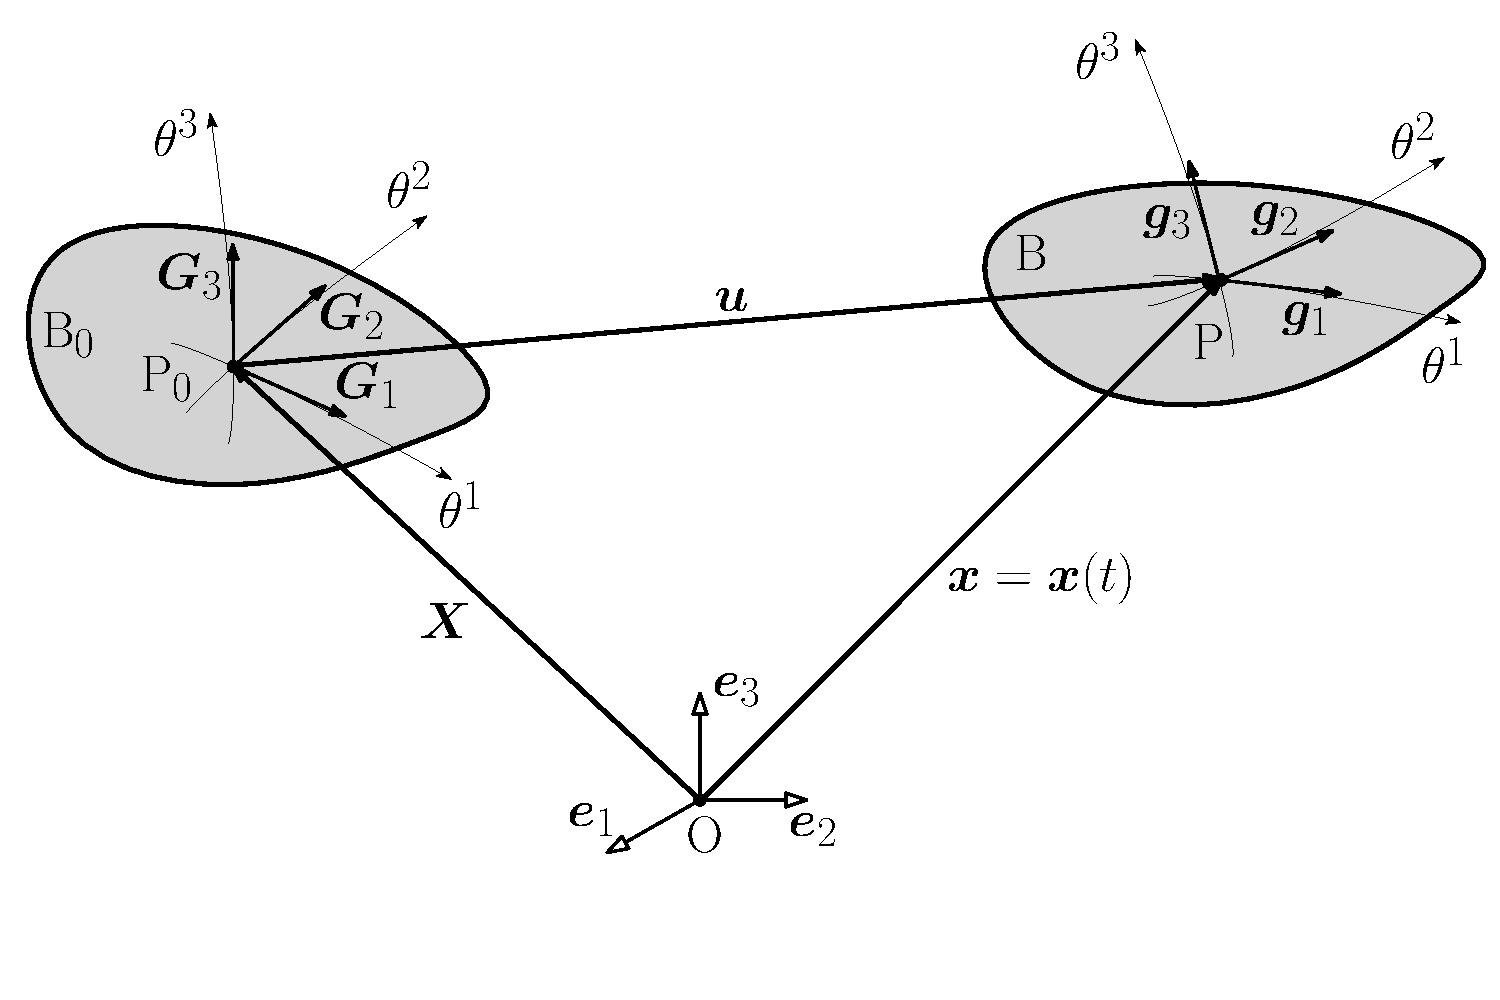
\includegraphics[width=\textwidth]{body_motion.pdf}
    \caption{Motion of a body}%
    \label{fig:body_motion}
\end{figure}

At any time \(t\), a mapping of the body B into a bounded region \(\mathcal{B}\) of the three-dimensional Euclidian space is assumed to be one to one and is referred to as a \emph{configuration}. Thus any point P of the body B can be associated with a position vector \(\bm{x} \in \mathbb{E}^{3}\). To describe the motion and deformation of the body B it is convenient to fix some configuration \(\mathcal{B}_{0}\) at time \(t_0\). This fixed configuration \(\mathcal{B}_{0}\) is called the \emph{reference configuration}. 

\paragraph*{Coordinates, Position Vectors and Displacement} With a coordinate system \(\theta^{i} (i = 1,2,3)\) the point P can be defined by its coordinates at time \(t_{0}\). Thus we can write
\begin{equation}
    \bm{x} = \bm{x}(\theta^{1}, \theta^{2}, \theta^{3}, t), \quad
     \theta^{i}=\theta^{i}(\bm{x}, t), \quad 
     i = 1,2,3
\end{equation}
and
\begin{equation}
    \bm{X} = \bm{x}(\theta^{1}, \theta^{2}, \theta^{3}, t_{0}) = \bm{X}(\theta^{1}, \theta^{2}, \theta^{3}), \quad \theta^{i}=\theta^{i}(\bm{X}, t_{0}), \quad i = 1,2,3
\end{equation}

where \(\bm{X}\) denotes the \emph{position vector} of the point \(\mathrm{P}_{0}\) in the reference configuration (\cref{fig:body_motion}). The coordinates \(\theta^{i}(i = 1,2,3)\) identify the point P at any time. They are often referred to as convective coordinates because the coordinate lines are embedded into the material and deform with the body.

The difference between the position vectors of the point P in the current and reference configuration 
\begin{equation}
    \bm{u} = \bm{u}(\theta^{1}, \theta^{2}, \theta^{3}, t) = \bm{x} - \bm{X}
\end{equation}
is called displacement.

The Euclidian space is characterized by the existence of an orthonormal basis given by a set of mutually orthogonal unit vectors, say \(\bm{e}_{i}\), with the property \(\bm{e}_{i} \cdot \bm{e}_{i} = \delta^{ij}\), where \(\delta^{ij}\) denotes the Kronecker delta and is defined by 
\begin{equation}
    \delta_{ij} =\delta^{ij} = \delta^{i}_{j} = \begin{cases}
        1,              & \text{for } i = j\\
        0,              & \text{for } i \neq j
    \end{cases}
\end{equation}

With respect to this basis, the position vectors and displacement can be expressed as
\begin{align}
\bm{X} &= X^{i} \bm{e}_{i}, \quad &X^{j} &= \bm{X} \cdot \bm{e}_j,  &j = 1,2,3 \\
\bm{u} &= u^{i} \bm{e}_{i}, \quad &u^{j} &= \bm{u} \cdot \bm{e}_j,  &j = 1,2,3 \\
\bm{x} &= x^{i} \bm{e}_{i}, \quad &x^{j} &= \bm{x} \cdot \bm{e}_j = X^{j} + u^{j}, &j = 1,2,3 
\end{align}
where henceforth Einstein's summation convention over repeated indexes is applied. \(X^{j}\) and \(x^{j} (j = 1,2,3)\) are called referential and current coordinate, respectively.

Other bases suitable for the description of deformation are formed by the vectors tangent to the coordinate lines in the reference and current cofigurations as shown in \cref{fig:body_motion}. These tangent vectors are defined by the derivatives of the position vectors with respect to the convective coordinates. For short, these derivatives will be denoted by
\(
    \dfrac{\partial \left( \bullet \right) }{\partial \theta^{i}}=\left( \bullet \right)_{,i}
\)
.Thus
\begin{equation}
\bm{G}_{i}=\dfrac{\partial \bm{X}}{\partial \theta ^{i}}=\bm{X}_{,i}={X^{j}}_{,i}\:{e_{j}}, \quad  
\bm{g}_{i}=\dfrac{\partial \bm{x}}{\partial \theta ^{i}}=x_{,i}={\bm{x}^{j}}_{,i}\:{e_{j}}, \quad 
i = 1,2,3
\end{equation}
where and henceforth we assume that the functions \(\bm{X} = \bm{X}(\theta^{1}, \theta^{2}, \theta^{3})\) and \(\bm{x} = \bm{x}(\theta^{1}, \theta^{2}, \theta^{3}, t)\) are sufficiently differentiable.

It is also useful to define the bases dual to \(\bm{G}_i\) and \(\bm{g}_i (i = 1,2,3)\):
\begin{equation}
    \bm{G}_{i} \cdot \bm{G}^{j} = \delta_{i}^{j}, \quad
    \bm{g}_{i} \cdot \bm{g}^{j} = \delta_{i}^{j}, \quad
    i,j = 1,2,3.
\end{equation}

Thus we can write
\begin{equation}
    \bm{G}^i = \dfrac{\partial \theta^{i}}{\partial X^{j}}\bm{e}^{j}, \quad
    \bm{g}^i = \dfrac{\partial \theta^{i}}{\partial x^{j}}\bm{e}^{j}, \quad
    i,j = 1,2,3.
\end{equation}

\paragraph*{Deformation Gradient}
The current postion \(\bm{x}\) of some point P and its displacement \(\bm{u}\) characterize only the \emph{motion} of the body in this point. In order to describe its deformation it is necessary to know how fast these vectors change in a neighbourhood of this point. For example, there is no deformation if all points get the same displacement. In this case we deal with the rigid body motion.

The deformation gradient is defined as the gradient of the position vector in the current configuration and is denoted by \(\mathbf{F}\):
\begin{equation}
    \mathbf{F} = \text{Grad}\,{\bm{x}} = 
    \text{F}^{i}_{.j}\,\bm{e}_{i} \otimes \bm{e}^{j}
\end{equation}
where the matrix \(\left[\text{F}^{i}_{.j}\right]\) is given by 

\begin{equation}
    \left[\text{F}^{i}_{.j}\right]\ = 
    \begin{bmatrix}
        \pdv{x^{1}}{X^{1}} & \pdv{x^{1}}{X^{2}} & \pdv{x^{1}}{X^{2}} \\[0.5em]
        \pdv{x^{2}}{X^{1}} & \pdv{x^{2}}{X^{2}} & \pdv{x^{2}}{X^{2}} \\[0.5em]
        \pdv{x^{3}}{X^{1}} & \pdv{x^{3}}{X^{2}} & \pdv{x^{3}}{X^{2}}
    \end{bmatrix} = 
    \begin{bmatrix}
        \pdv{u^{1}}{X^{1}} + 1 & \pdv{u^{1}}{X^{2}} & \pdv{u^{1}}{X^{2}} \\[0.5em]
        \pdv{u^{2}}{X^{1}} & \pdv{u^{2}}{X^{2}} + 1 & \pdv{u^{2}}{X^{2}} \\[0.5em]
        \pdv{u^{3}}{X^{1}} & \pdv{u^{3}}{X^{2}} & \pdv{u^{3}}{X^{2}} + 1
    \end{bmatrix}
\end{equation}

The deformation gradient can also be written in a more compact form using the tangent vectors.
\begin{equation}
    \mathbf{F} = \bm{g}_{i} \otimes \bm{G}^{j}
\end{equation}
\paragraph*{Deformation of line, surface and volume elements} 
If an infinitesimal line element \(d\bm{X}\) in the reference configuration is considered along with its counterpart \(d\bm{x}\) in the current configuration, it can be shown that
\begin{equation}
    d\bm{x} = \mathbf{F} d\bm{X}, \quad
    d\bm{X} = \mathbf{F}^{-1} d\bm{x}
    \label{eq:linemap}
\end{equation}
and hence suggesting the following symbolic representation for the deformation gradient
\begin{equation}
    \mathbf{F} = \text{Grad}\,{\bm{x}} = \pdv{\bm{x}}{\bm{X}}, \quad
    \mathbf{F}^{-1} = \text{grad}\,{\bm{X}} = \pdv{\bm{X}}{\bm{x}}.
    \label{eq:defgrd_symbolic}
\end{equation}
The deformation gradient is also suitable to describe the deformation of volume and surface elements. If \(dV_{0}\) is the volume of an infinitesimal volume element in the reference configuration and \(dV\) is the corresponding volume of the same volume element after deformation in the current configuration, then it can be shown that
\begin{equation}
    \dfrac{dV}{dV_{0}} = \text{det}\mathbf{F} = |\text{F}^{i}_{.j}| =  J
    \label{eq:volumemap}
\end{equation}

In the same way if we consider vectorial surface elements \(d\bm{S}\) and \(d\bm{s}\) along with the positive unit normals to these surfaces as \(\bm{N}\) and \(\bm{s}\) in the reference and current configuration respectively, we have the relation 
\begin{equation}
    d\bm{s} = J\mathbf{F}^{-T}d\bm{S},\quad ds\bm{n} = J\mathbf{F}^{-T}\bm{N}dS
    \label{eq:nanson}
\end{equation}
which is also referred to as Nanson's formula.

\paragraph*{Strain}
A material is said to be strained in some point \(\text{P}(\bm{X})\) if at least one of the infinitesimal line elements \(d\bm{X}\) based on \(\bm{X}\) changes its length after deformation. For the square lengths we can write by virtue of \cref{eq:linemap} we have
\begin{align}
    \nonumber||d\bm{x}||^{2} 
             &= d\bm{x} \cdot d\bm{x} 
              = (\mathbf{F} d\bm{X}) \cdot (\mathbf{F} d\bm{X})\\
    \nonumber&= (d\bm{X}\mathbf{F}^{T}) \cdot (\mathbf{F} d\bm{X}) 
              = d\bm{X} (\mathbf{F}^{T} \mathbf{F}) d\bm{X}\\
             &= d\bm{X} \mathbf{C} d\bm{X},\label{eq:sqlen_cur}\\[1em]
    \nonumber||d\bm{X}||^{2} 
             &= d\bm{X} \cdot d\bm{X} 
              = (\mathbf{F}^{-1} d\bm{x}) \cdot (\mathbf{F}^{-1} d\bm{x})\\
    \nonumber&= (d\bm{x}\mathbf{F}^{-T}) \cdot (\mathbf{F}^{-1} d\bm{x}) 
              = d\bm{x} (\mathbf{F}^{-T} \mathbf{F}^{-1}) d\bm{x}\\
             &= d\bm{x} \mathbf{b}^{-1} d\bm{x},\label{eq:sqlen_ref}
\end{align}
where the symmetric tensors 
\begin{equation}
    \mathbf{C} = \mathbf{F}^{T}\mathbf{F}, \quad
    \mathbf{b} = \mathbf{F}\mathbf{F}^{T}
    \label{eq:def_right_left_cauchygreen}
\end{equation}
are referred to as the right and left Cauchy-Green deformation tensor respectively.
They can also be expressed in terms of the tangent vectors as
\begin{align}
    \mathbf{C} &= g_{ij} \;\bm{G}^{i} \otimes \bm{G}^{j}\\
    \mathbf{b} &= G^{ij} \;\bm{g}_{i} \otimes \bm{g}_{j}
\end{align}
where the abbreviations 
\begin{equation}
    g_{ij} = \bm{g}_{i} \cdot \bm{g}_{j}, \quad
    G^{ij} = \bm{G}^{i} \cdot \bm{G}^{j}, \quad
    i,j = 1,2,3
\end{equation}
In order to express strains, the difference of square lengths are in \cref{eq:sqlen_cur} and \cref{eq:sqlen_ref} are considered and after mathematical manipulation the we get the symmetric tensors
\begin{alignat}{2}
    \mathbf{E} 
    &=\dfrac{1}{2} (\mathbf{C} - \mathbf{I}) 
    &&=\dfrac{1}{2} (\mathbf{F}^{T}\mathbf{F} - \mathbf{I})\\
    \mathbf{e}
    &=\dfrac{1}{2} (\mathbf{I} - \mathbf{b}^{-1}) 
    &&=\dfrac{1}{2} (\mathbf{I} - \mathbf{F}^{-T} \mathbf{F}^{-1})
\end{alignat}

which are called the Green-Lagrange strain tensor and Almansi strain tensor respectively. The material body is thus said to be unstrained if \(\mathbf{E} = \mathbf{e} = \mathbf{0}\) and the deformation gradient represents an orthogonal tensor, and hence, \(\mathbf{F}^{T}\mathbf{F} = \mathbf{I}\). If this is the case in every point of the body, then we deal with the rigid body motion.

\paragraph*{Stretch and Shear}
With the aid of the Cauchy-Green tensor, it is possible to express the stretch of a line element as well as change in angle between two orthogonal line elements defined in the reference configuration. The ratio of the deformed to the reference length of a line element is called stretch. If \(\bm{N}\) and \(\bm{n}\) are unit vectors along the infinitesimal line element \(d\bm{X}\) and its counterpart in the current configuration \(d\bm{x}\), respectively. Furthermore with \(d\bm{X}=||d\bm{X}||\bm{N}\) and \(d\bm{x}=||d\bm{x}||\bm{n}\), the stretch in the direction of \(\bm{N}\) takes the form
\begin{align}
    \nonumber\lambda(\bm{N}) &= \sqrt{\dfrac{||d\bm{x}||^{2}}{||d\bm{X}||^{2}}}\\
                    &= {(\bm{N}\bm{C}\bm{N})}^{\textstyle{\frac{1}{2}}}
\end{align}
and similarly the strecth in the direction of \(\bm{n}\) it can be shown
\begin{equation}
    \lambda(\bm{n}) = {(\bm{n}\bm{b}^{-1}\bm{n})}^{\textstyle-{\frac{1}{2}}}
\end{equation}
By representing the Cauchy-Green tensor with respect to an orthonormal basis \(\bm{N}_{i} \cdot \bm{N}_{j} = \delta_{ij},\;(i,j = 1,2,3)\), we get 
\begin{equation}
    \lambda(\bm{N}_i) 
    = {(\bm{N}_i\bm{C}\bm{N}_i)}^{\textstyle{\frac{1}{2}}}
    = \sqrt{\text{C}_{ii}}, \quad \text{no sum over } i = 1,2,3
\end{equation}
Thus the square roots of the diagonal components of the Cauchy-Green tensor expressed in an orthonormal basis represent the stretches in the corresponding directions \(\bm{N}_i\;(i=1,2,3)\)
The decrease in the angle after deformation between two orthogonal line elements, say \(d\bm{X}_{i}=||d\bm{X}_{i}||\bm{N}_{i},\: (i=1,2)\) defined in the reference configuration is given by
\begin{equation}
    \sin\varphi_{12} = \dfrac{\text{C}_{12}}{\sqrt{\text{C}_{11}\text{C}_{22}}}
\end{equation}

\paragraph*{Spectral Decomposition of Strain Tensors}
By setting up an eigen value problem for the right Cauchy-Green tensor we have
\begin{equation}
    \mathbf{C} \bm{N} = \Lambda \bm{N}, \quad \bm{N} \neq 0
\end{equation}
where a non-zero vector \(\bm{N}\) is called an eigen vector and \(\Lambda\) denotes the corresponding eigen value. To solve this eigen value problem, \(\mathbf{C}\) and \(\bm{N}\) are represented with respect to a basis. This finally results in 
\begin{equation}
    (\text{C}^{i}_{j} - \Lambda\delta^{i}_{j})N^{j} = 0, \quad
    i = 1,2,3
\end{equation}
which is a homogenous linear equation system with respect to the components of the eigen vector \(\bm{N}\). This equation system has a non-trivial solution if an only if
\begin{equation}
    |\text{C}^{i}_{j} - \Lambda\delta^{i}_{j}| = 0
\end{equation}
or equivalently
\begin{equation}
    \begin{vmatrix}
        \text{C}^{1}_{1}  - \Lambda & \text{C}^{1}_{2} & \text{C}^{1}_{3} \\[0.5em]
        \text{C}^{2}_{1} & \text{C}^{2}_{2} - \Lambda & \text{C}^{2}_{3} \\[0.5em]
        \text{C}^{3}_{1} & \text{C}^{3}_{2} & \text{C}^{3}_{3} - \Lambda
    \end{vmatrix} = 0,
\end{equation}
where \(|\bullet|\) denotes the determinant of a matrix. Writing out this determinant and collecting the terms according to the powers of \(\Lambda\) one obtains the so-called characteristic equation which is given by
\begin{equation}
    \Lambda^{3} 
    - \text{I}_{\mathbf{C}}\Lambda^{2}
    + \text{II}_{\mathbf{C}}\Lambda
    - \text{III}_{\mathbf{C}} = 0,
\end{equation}
where the coefficients take the form
\begin{align}
    \text{I}_{\mathbf{C}} &= \text{C}_{i}^{i} = \text{tr}\mathbf{C} \\
    \text{II}_{\mathbf{C}} &= \dfrac{1}{2}(\text{C}^{i}_{i}\text{C}^{j}_{j} - \text{C}^{i}_{j}\text{C}^{j}_{i}) = \dfrac{1}{2}[(\text{tr}\mathbf{C})^{2} - \text{tr}\mathbf{C}^{2}]\\  
    \text{III}_{\mathbf{C}} &= |\text{C}^{i}_{j}| = \text{det}\mathbf{C}
\end{align}
The solution of the eigen value problem resulting from the characteristic equation does not depend on the choice of the coordinate system. Therefore, also the coefficients of the characteristic equation are independent of the coordinate system and, hence, are called the principal invariants of \(\mathbf{C}\). Since the tensor \(\mathbf{C}\) is symmetric its characteristic equation has three real roots \(\Lambda_{i}(i=1,2,3)\). The characteristic equation can also be represented in terms of the roots by 
\begin{equation}
    (\Lambda_{1} - \Lambda)(\Lambda_{2} - \Lambda)(\Lambda_{3} - \Lambda) = 0
\end{equation}
By virtue of the tensor identity, \(\text{tr}(\mathbf{AB}) = \text{tr}(\mathbf{BA})\) and taking \cref{eq:volumemap} into account it can be shown that
\begin{align}
    \text{tr}\mathbf{C} &= \text{tr}\mathbf{b}\\
    \text{tr}\mathbf{C}^2 &= \text{tr}\mathbf{b}^2\\ 
    \text{det}\mathbf{C} &= \text{det}\mathbf{b} = J^2
\end{align}
Thus, we conclude the tensors \(\mathbf{C}\) and \(\mathbf{b}\) have the same principal invariants
\begin{equation}
    \text{I}_{\mathbf{C}} = \text{I}_{\mathbf{b}}, \quad 
    \text{II}_{\mathbf{C}} = \text{II}_{\mathbf{b}}, \quad
    \text{III}_{\mathbf{C}} = \text{III}_{\mathbf{b}}
    \label{eq:straininv}
\end{equation}
which are also referred to as strain invariants. \cref{eq:straininv} immediately implies the equivalence of the eigen values of the right and left Cauchy-Green tensors. This is an important property and is useful for material modelling.

The eigen vectors of symmetric tensors such as \(\mathbf{C}\) and \(\mathbf{b}\) are linearly independent and can be represented by an orthonormal basis. Thus, we can write the spectral decomposition as
\begin{equation}
    \mathbf{C} = \sum_{n = 1}^{3}\Lambda_{i}\bm{N}_{i} \otimes \bm{N}_{i}, \quad
    \mathbf{b} = \sum_{n = 1}^{3}\Lambda_{i}\bm{n}_{i} \otimes \bm{n}_{i},
    \label{eq:spectraldecomposition}
\end{equation}
where
\begin{equation}
    \bm{N}_{i} \cdot \bm{N}_{j} = \delta_{ij}, \quad
    \bm{n}_{i} \cdot \bm{n}_{j} = \delta_{ij}, \quad
    i,j = 1,2,3.
\end{equation}
In view of \cref{eq:sqlen_cur} and \cref{eq:sqlen_ref} the tensors \(\mathbf{C}\) and \(\mathbf{b}\) are positive definite which implies that their eigen values \(\Lambda_{i}(i=1,2,3)\) are positive. Using this property we can write the powers of these tensors on the basis of the spectral decomposition by
\begin{equation}
    \mathbf{C}^{\alpha} = \sum_{n = 1}^{3}\Lambda_{i}^{\alpha}\bm{N}_{i} \otimes \bm{N}_{i}, \quad
    \mathbf{b}^{\alpha} = \sum_{n = 1}^{3}\Lambda_{i}^{\alpha}\bm{n}_{i} \otimes \bm{n}_{i},
    \label{eq:power_C}
\end{equation}
\begin{figure}[htpb]
    \centering
    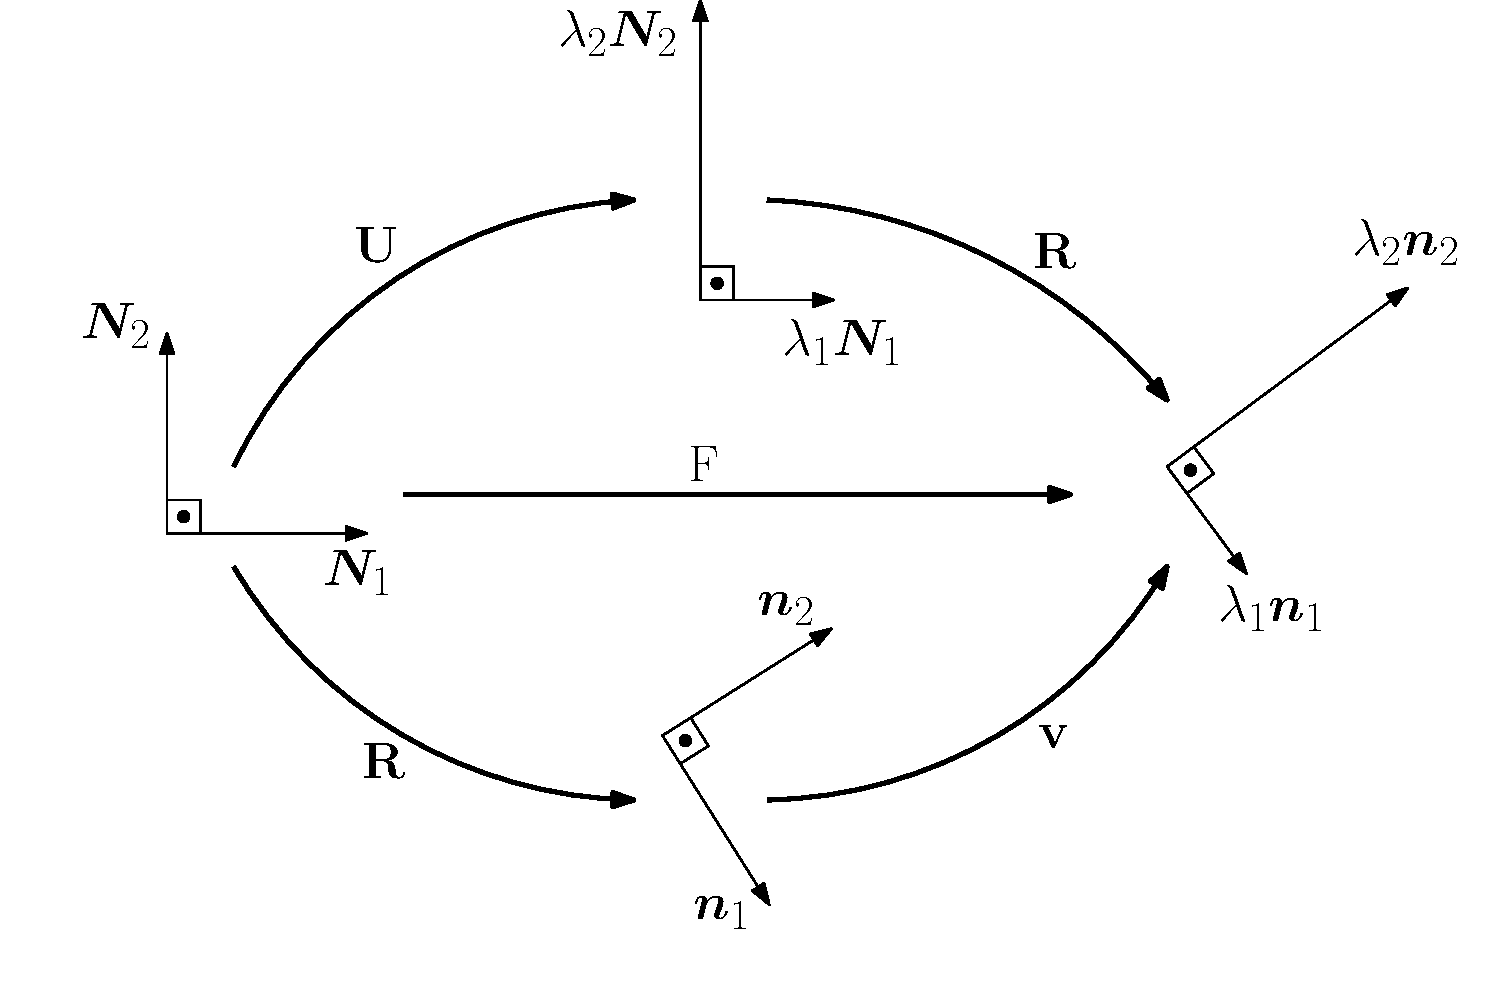
\includegraphics[width=\textwidth]{polar_decompositioin.pdf}
    \caption{Polar decomposition}%
    \label{fig:polar_decompositioin}
\end{figure}

\paragraph*{Polar Decomposition of Deformation Gradient} 
The deformation gradient can be further decomposed into a rotation and stretch tensor. By setting in \cref{eq:power_C} \(\alpha=\frac{1}{2}\) one defines the so-called right and left stretch tensors
\begin{equation}
    \mathbf{U} 
    = \mathbf{C}^{\frac{1}{2}} 
    = \sum_{i=1}^{3}  \lambda_{i} \bm{N}_{i} \otimes \bm{N}_{i}, \quad
    \mathbf{v} 
    = \mathbf{b}^{\frac{1}{2}} 
    = \sum_{i=1}^{3}  \lambda_{i} \bm{n}_{i} \otimes \bm{n}_{i},
    \label{eq:defUv}
\end{equation}
where 
\begin{equation}
    \lambda_{i} = \sqrt{\Lambda_{i}}, \quad i=1,2,3.
\end{equation}
Further one can show that 
\begin{equation}
    \mathbf{R} = \mathbf{F}\mathbf{U}^{-1}
    \label{eq:rotation}
\end{equation}
represents a proper orthogonal tensor as it can be shown that \(\mathbf{R}\mathbf{R}^{T}=\mathbf{I}\) and \(\text{det}(\mathbf{R}) \geq 0\). 
From \cref{eq:rotation} we further get
\begin{equation}
    \mathbf{F} 
    = \mathbf{R}\mathbf{U} 
    = (\mathbf{R}\mathbf{U}\mathbf{R}^{T})\mathbf{R}.
\end{equation}
Due to the symmetry of \(\mathbf{U}\) it can be shown that the tensor \(\mathbf{R}\mathbf{U}\mathbf{R}^{T}\) is also symmetric and one can derive that \((\mathbf{R}\mathbf{U}\mathbf{R}^{T})^{2} = \mathbf{b}\). In view of \cref{eq:defUv}{\({}_2\)}, there exists only one real symmetric tensor whose square is \(\mathbf{b}\). Hence \(\mathbf{R}\mathbf{U}\mathbf{R}^{T} = \mathbf{v}\). This results in the following identity
\begin{equation}
    \mathbf{F} 
    = \mathbf{R}\mathbf{U}
    = \mathbf{v}\mathbf{R}
    \label{eq:polar_decomposition}
\end{equation}
which is referred to as the \emph{polar decomposition} of the deformation gradient. By virtue of \cref{eq:polar_decomposition} we also obtain
\begin{equation}
    \mathbf{U} = \mathbf{R}^{T}\mathbf{v}\mathbf{R}, \quad
    \mathbf{C} = \mathbf{R}^{T}\mathbf{b}\mathbf{R}, \quad
    \mathbf{v} = \mathbf{R}\mathbf{U}\mathbf{R}^{T}, \quad
    \mathbf{b} = \mathbf{R}\mathbf{C}\mathbf{R}^{T}
    \label{eq:rotation_stretch_cauchy}
\end{equation}
Considering a special case of pairwise distinct eigen values of the stretch tensors \(\lambda{1}\neq \lambda{2} \neq \lambda{3}\neq \lambda{1}\) and using \cref{eq:rotation_stretch_cauchy} it can be shown that 
\begin{equation}
    \mathbf{v} = \mathbf{R}\mathbf{U}\mathbf{R}^{T} 
    = \sum_{i=1}^{3}  \lambda_{i} (\mathbf{R}\bm{N}_{i}) \otimes (\mathbf{R}\bm{N}_{i})
\end{equation}
Comparing this with \cref{eq:defUv}\({}_2\) we obtain
\begin{equation}
    \bm{n}_{i} = \mathbf{R}\bm{N}_{i}, \quad
    \bm{V}_{i} = \mathbf{R}^{T}\bm{n}_{i}, \quad
    i = 1,2,3.
\end{equation}
and consequently
\begin{equation}
    \mathbf{R} = \sum_{i=1}^{3}  \bm{n}_{i} \otimes \bm{N}_{i}, \quad
    \mathbf{F} = \sum_{i=1}^{3}  \lambda_{i} \bm{n}_{i} \otimes \bm{N}_{i}, \quad
    \prstretche{}{1} \neq \prstretche{}{2} \neq \prstretche{}{3} \neq \prstretche{}{1} 
\end{equation}
Thus the deformation of an eigen vector \(\bm{N}_{i} (i=1,2,3)\) can be accomplished in two steps: rotation by \(\mathbf{R}\) to \(\bm{n}_{i}\) and stretching by \(\mathbf{v}\) to \(\lambda\bm{n}_{i}\) or vice versa: stretching by \(\mathbf{U}\) to \(\lambda\bm{N}_{i}\) and rotation by \(\mathbf{R}\) to \(\lambda\bm{n}_{i}\) as shown illustratively in \cref{fig:polar_decompositioin} and mathematically as
\begin{alignat}{3}
    \nonumber\mathbf{F}\bm{N}_{i} 
    &= \mathbf{v}(\mathbf{R}\bm{N}_{i}) 
    &&=  \mathbf{v}\bm{\lambda}_{i} 
    &&= \lambda_{i}\bm{n}_{i} \quad \text{or} \\
    \mathbf{F}\bm{N}_{i}
    &= \mathbf{R}(\mathbf{U}\bm{N}_{i}) 
    &&= \lambda_{i}\mathbf{R}\bm{N}_{i}
    &&= \lambda_{i}\bm{n}_{i}, \quad
    i = 1,2,3
\end{alignat}

For this reason, \(\mathbf{R}\) is called the rotation tensor and the eigen values \(\lambda_{i}(i=1,2,3)\) of the stretch tensors \(\mathbf{U}\) and \(\mathbf{v}\) are referred to as the principal stretches.
\paragraph*{Velocity Gradient}
The velocity of a material particle P is defined by
\begin{equation}
    \bm{v} = \pdv{\bm{x}(\bm{X},t)}{t} = \dot{\bm{x}}
    \label{eq:velocity}
\end{equation}
The time derivative denoted by the superposed dot is called the material time derivative since the position vector \(\mathbf{X}\) in the reference configuration is held constant. The material velocity gradient is defined similar to the deformation gradient by
\begin{equation}
    \mathbf{L} = \text{Grad}\bm{v} = \pdv{\bm{v}}{\bm{X}}.\
    \label{eq:def_matVelGradient}
\end{equation}
Taking into account \cref{eq:velocity} and \cref{eq:defgrd_symbolic} we can write 
\begin{equation}
    \mathbf{L} = \text{Grad}\dot{\bm{x}} 
    = \pdv*{\left[\pdv{\bm{x}(\bm{X},t)}{\bm{t}}\right]}{\bm{X}}
    = \pdv*{\left(\pdv{\bm{x}}{\bm{X}}\right)}{t}
    = \dot{\mathbf{F}}
    \label{eq:matVelGradient}
\end{equation}
Of special interest is also the spatial velocity gradient defined by 
\begin{equation}
    \mathbf{l} = \text{grad}\bm{v} = \pdv{\bm{v}}{\bm{x}}
    \label{eq:def_spatVelGradient}
\end{equation}
Using \cref{eq:defgrd_symbolic}\({}_{2}\) and \cref{eq:def_matVelGradient} we thus obtain
\begin{equation}
    \mathbf{l} = \pdv{\bm{v}}{\bm{X}}\pdv{\bm{X}}{\bm{x}}
    = \dot{\mathbf{F}}\mathbf{F}^{-1}
    \label{eq:spatVelGradient}
\end{equation}
According to \cref{eq:def_matVelGradient} and \cref{eq:def_spatVelGradient} it follows that 
\begin{equation}
    d\bm{v} = d\dot{\bm{x}} = \mathbf{l}d\bm{x} = \mathbf{L}d\bm{X}.
\end{equation} 
Furthermore, the spatial gradient of velocity is usually decomposed into a symmetric \(\mathbf{d}=\mathbf{d}^{T}\) and a skew-symmetric part \(\mathbf{w}=-\mathbf{w}^{T}\) by 
\begin{equation}
    \mathbf{l} = \mathbf{d} + \mathbf{w},
    \label{spatial_velocity_gradient}
\end{equation} 
where
\begin{align}
    \nonumber\mathbf{d} 
    &= \dfrac{1}{2}\left(\mathbf{l}+\mathbf{l}^{T}\right) 
    = \dfrac{1}{2}\left(\dot{\mathbf{F}}\mathbf{F}^{-1} +\mathbf{F}^{-T}\dot{\mathbf{F}}^{T}\right)
    = \dfrac{1}{2}\mathbf{F}^{-T}\dot{\mathbf{C}}\mathbf{F}^{-1}\\
    &= \mathbf{F}^{-T}\dot{\mathbf{E}}\mathbf{F}^{-1}
    \label{eq:rate_of_deformation}
\end{align}
is called the rate of deformation tensor and 
\begin{equation}
    \nonumber\mathbf{w} 
    = -\mathbf{w}^{T}
    = \dfrac{1}{2}\left(\mathbf{l}-\mathbf{l}^{T}\right)
    = \dfrac{1}{2}\left(\dot{\mathbf{F}}\mathbf{F}^{-1} -\mathbf{F}^{-T}\dot{\mathbf{F}}^{T}\right)
    \label{vorticity}
\end{equation}
is called spin (vorticity) tensor.

\subsection{Stress}
\begin{figure}[htpb]
    \centering
    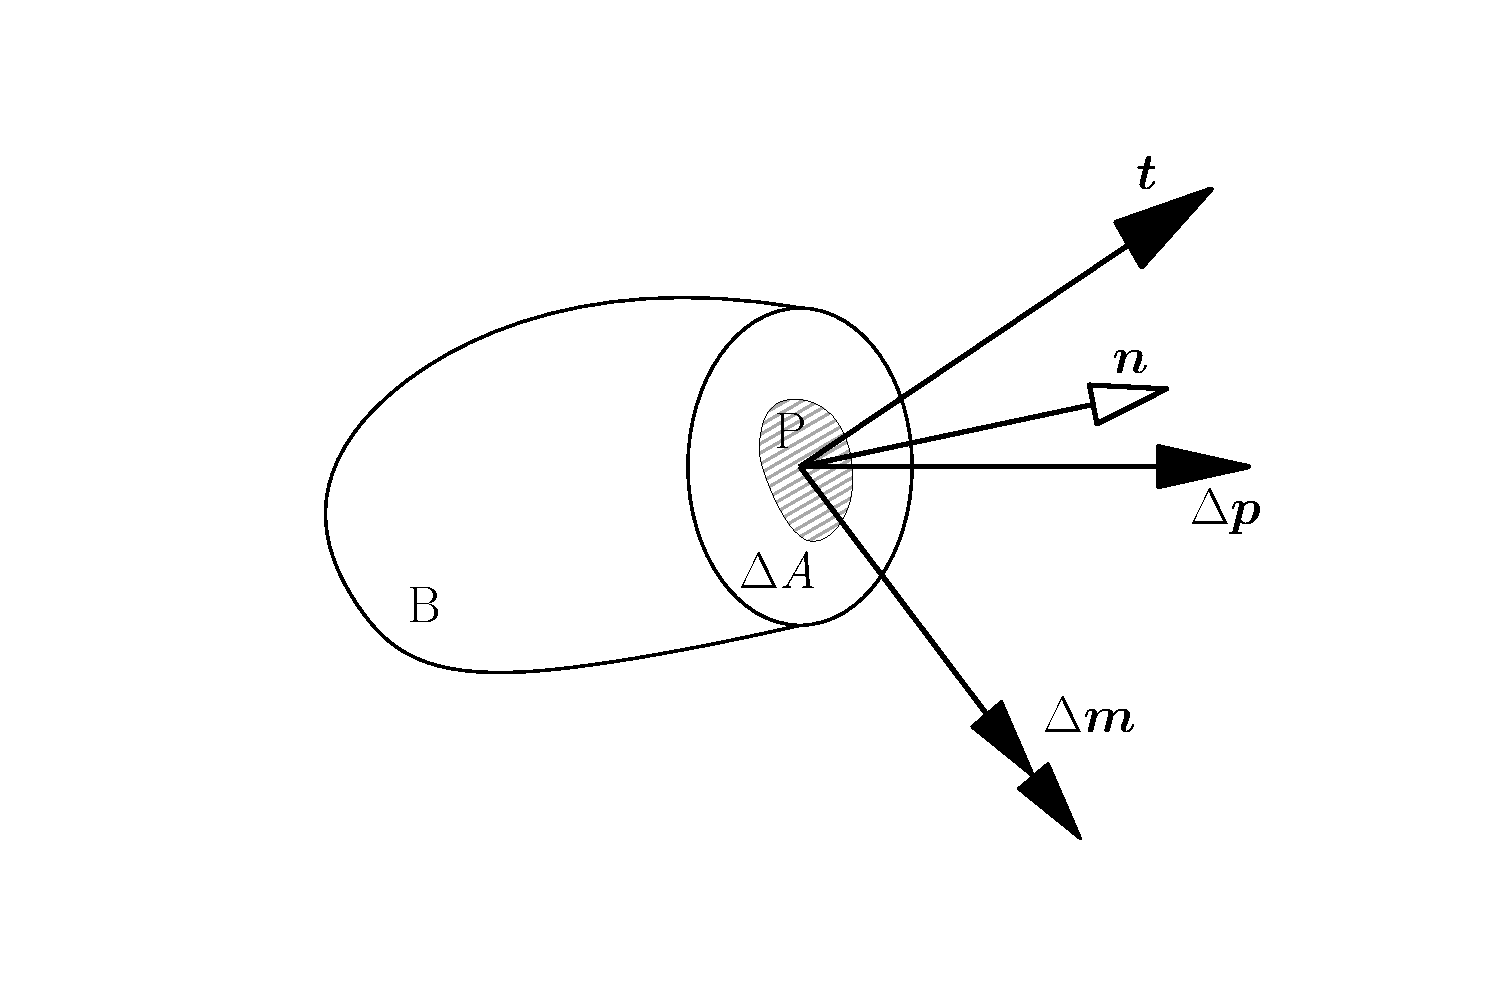
\includegraphics[width=0.7\textwidth]{cauchy_stress_vector.pdf}
    \caption{Cauchy stress vector}%
    \label{fig:cauchy_stress_vector}
\end{figure}
Let us consider a body B in the current configuration at a time \(t\). In order to define stress in some point P let us further imagine a smooth surface going through P and separating B into two parts, of which one part is as shown in \cref{fig:cauchy_stress_vector}. One can then define a force \(\Delta\bm{p}\) and a couple \(\Delta\bm{m}\) resulting from the forces exerted by material on one side of the surface \(\Delta A\) on the material on the other side. Let the area \(\Delta A\) tend to zero permanently keeping P as an inner point. A basic postulate of continuum mechanics is that the limit 
\begin{equation}
    \bm{t} = \lim_{\Delta A \to 0}\frac{\Delta\bm{p}}{\Delta A}
\end{equation}
exists and is finite. The so-defined vector \(\bm{t}\) is called the Cauchy stress vector. The Cauchy's fundamental postulate states that the vector t depends on the surface only through the unit outward normal \(\bm{n}\) as shown in \cref{fig:cauchy_stress_vector}. In other words, the Cauchy stress vector is the same for all surface through P which have a normal \(\bm{n}\) in P. As a result one can write
\begin{equation}
    \bm{t} = \bm{t}(\bm{x},\bm{n}) = \bm{t}(\bm{X},\bm{n},t).
    \label{eq:cauchy_stress_vector}
\end{equation}
According to Cauchy's theorem the mapping \(\bm{n}\rightarrow \bm{t}\) is linear provided the function \cref{eq:cauchy_stress_vector} is continuous at \(\bm{X}\). Hence this mapping can be described by a second-order tensor as 
\begin{equation}
    \bm{t} = \bm{\sigma}\bm{n}
    \label{eq:cauchy_stress_tensor}
\end{equation}
The tensor \(\bm{\sigma}\) is called the Cauchy stress tensor and is related to the surface in the current configuration. 

\begin{figure}[htpb]
    \centering
    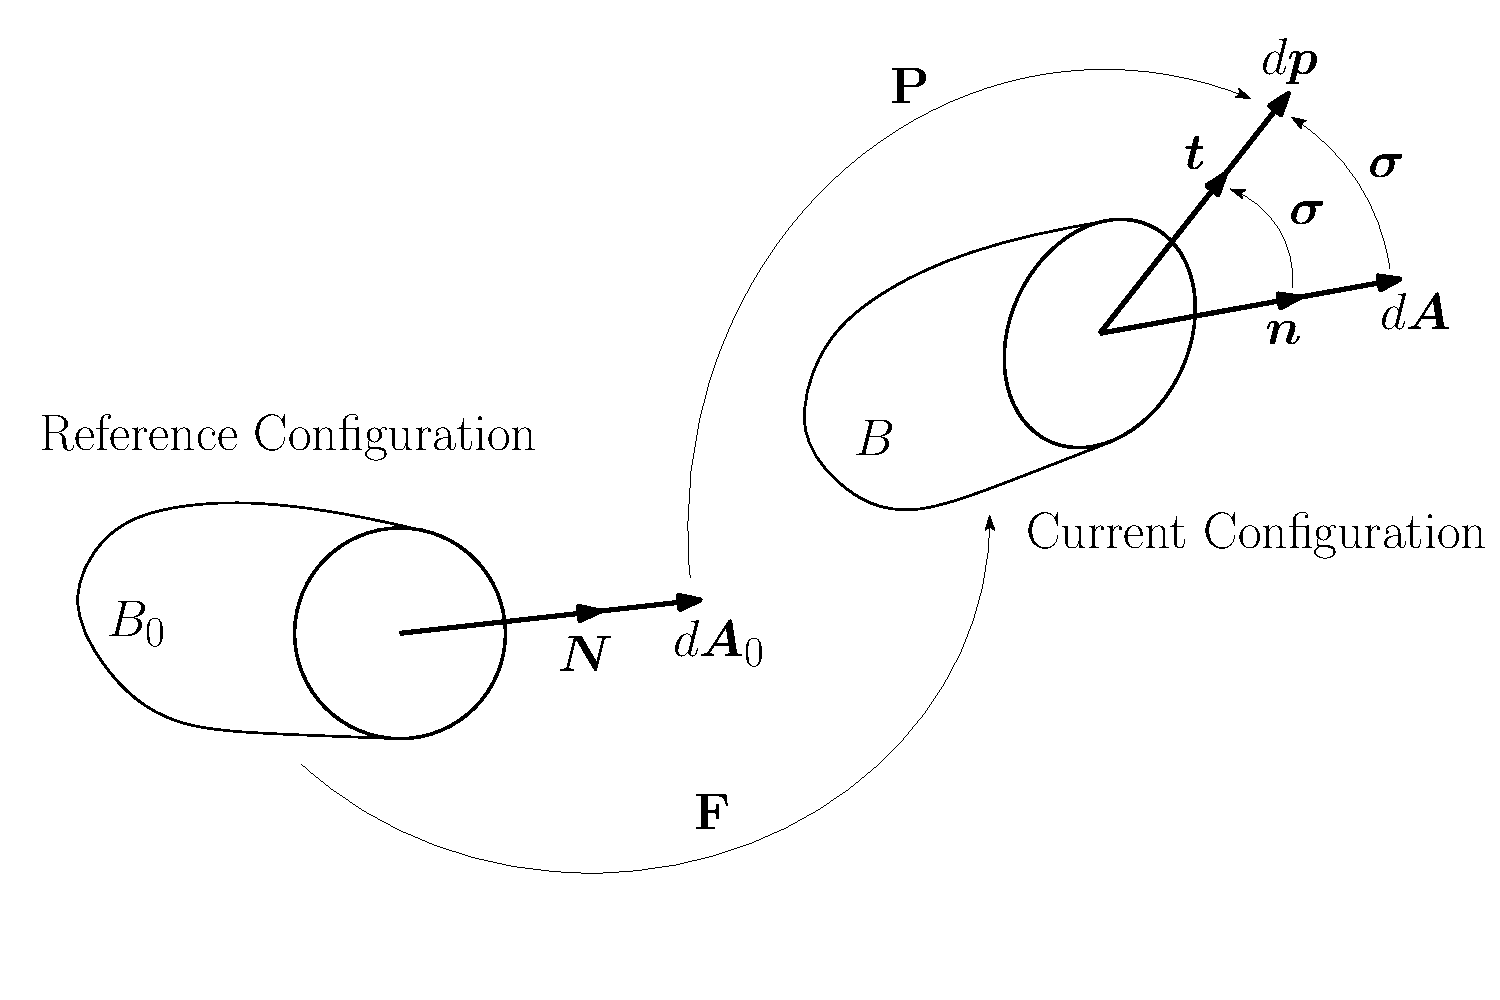
\includegraphics[width=\textwidth]{first_piola_kirchoff.pdf}
    \caption{First Piola-Kirchoff stress tensor}%
    \label{fig:first_piola_kirchoff_stress}
\end{figure}
Sometimes it is useful to define a stress tensor with respect to the reference configuration. For this consider a function \(d\bm{p}=d\bm{p}(d\bm{A})\) where
\begin{equation}
    d\bm{p} = \bm{t}dA
\end{equation}
and \(d\bm{A}=\bm{n}dA\) represents a vectorial surface element corresponding to the differential area \(dA\). The function \(\bm{t} = \bm{t}(\bm{n})\) is linear if and only if the function \(d\bm{p}=d\bm{p}(d\bm{A})\) is linear. Furthermore, using Nanson's formula we have
\begin{equation}
    d\bm{p} = \bm{t}dA = \bm{\sigma}d\bm{A} = J\bm{\sigma}\mathbf{F}^{-T}d\bm{A}_{0}
\end{equation}
With the aid of the definition
\begin{equation}
    \mathbf{P}=J\bm{\sigma}\mathbf{F}^{-T} = \bm{\tau}\mathbf{F}^{-T}
    \label{eq:def_firstpiolakirchoffstress}
\end{equation}
where 
\begin{equation}
    \bm{\tau} = J\bm{\sigma}
    \label{eq:kirchoff_stress}
\end{equation}
is referred to as the Kirchoff stress tensor, we can write
\begin{equation}
    d\bm{p} = \mathbf{P}d\bm{A}_{0}.
    \label{eq:firstpiolakirchoffmap}
\end{equation}
\(\mathbf{P}\) is called the first Piola-Kirchoff stress tensor and it relates the stress vector to the surface in the reference configuration as shown in \cref{eq:firstpiolakirchoffmap}. 
Furthermore the second Piola-Kirchoff stress tensor is defined by 
\begin{equation}
    \mathbf{S}  = J\mathbf{F}^{-1}\bm{\sigma}\mathbf{F}^{-T}
    =\mathbf{F}^{-1} \tautot \mathbf{F}^{-T}
     = \mathbf{F}^{-1}\mathbf{P}
    \label{eq:secondpiolakirchoff_stress}
\end{equation}
which is an important stress tensor quantity but has no physical significance.

\subsection{Balance Laws}
\paragraph*{Linear Momentum Balance}
If we consider the current configuration of the body B with the volume \(V\), mass \(M\) and boundary surface \(A\), the linear momentum of the body is defined by 
\begin{equation}
    \int_{M}^{} \bm{v} \,dm 
\end{equation}
where \(\bm{v} = \pdv{\bm{x}}{t} = \dot{\bm{x}}\) denotes the velocity of a particle with the position vector \(\bm{x}\) and mass \(dm\). Using the relation \(dm = \rho dV\), where \(\rho\) denotes the density, we can write 
\begin{equation}
    \int_{M}^{} \bm{v} \,dm 
    =  \int_{M}^{} \dot{\bm{x}} \,dm 
    =  \int_{V}^{} \rho\dot{\bm{x}} \,dV 
\end{equation}
According to a fundamental principle of continuum mechanics the rate of change of the linear momentum is equal to the resultant force applied on the body. This resultant force comprises a body force (without inertia) and a surface force and is thus written by 
\begin{equation}
    \int_{V}^{} \bm{f} \,dV 
    + \int_{A}^{} \bm{t} \,dA
\end{equation}
Thus, the linear momentum balance (the first Euler law of motion) takes the form
\begin{equation}
    \pdv*{\int_{V}^{} \rho\dot{\bm{x}} \,dV }{t}
    = \int_{V}^{} \bm{f} \,dV 
    + \int_{A}^{} \bm{t} \,dA
    \label{eq:lin_momentum_balance}
\end{equation}
Using the mass conservation law we can rewrite the left hand side of \cref{eq:lin_momentum_balance} by
\begin{equation}
    \pdv*{\int_{V}^{} \rho\dot{\bm{x}} \,dV }{t} 
    = \pdv*{ \int_{M}^{} \bm{v} \,dm}{t} 
    =  \int_{M}^{} \dot{\bm{v}} \,dm 
    = \int_{V}^{} \rho\ddot{\bm{x}} \,dV
    = \int_{V}^{} \rho \bm{a} \,dV
\end{equation}
where \(\bm{a} = \dot{\bm{v}} = \ddot{\bm{a}}\) represents the acceleration vector of particle, which finally leads to 
\begin{equation}
    \int_{V}^{} \rho\ddot{\bm{x}} \,dV = \int_{V}^{} \bm{f} \,dV 
    + \int_{A}^{} \bm{t} \,dA
\end{equation}
By means of the Cauchy theorem \cref{eq:cauchy_stress_tensor} and Gauss divergence theorem from calculus we can write 
\begin{equation}
        \int_{V}^{} \rho\ddot{\bm{x}} \,dV
        = \int_{V}^{} \bm{f} \,dV 
        + \int_{V}^{} \text{div}\bm{\sigma} \,dV
\end{equation}
and consequently
\begin{equation}
    \int_{V}^{} (\text{div}\bm{\sigma} + \bm{f} -\rho\ddot{\bm{x}}) \,dV
    \label{eq:simplified_lin_momentum_balance}
\end{equation}
This equation holds for the whole body and any arbitrary part of it with the volume \(dV\). Assuming that the integrand in \cref{eq:simplified_lin_momentum_balance} is a continuous function in space we have
\begin{equation}
    \text{div}\bm{\sigma} + \bm{f} = \rho\ddot{\bm{x}}
    \label{eq:result_lin_momentum_balance}
\end{equation}
The equation of motion \cref{eq:result_lin_momentum_balance} can also be written in terms of the first Piola-Kirchoff stress tensor \cref{eq:def_firstpiolakirchoffstress} and is given by 
\begin{equation}
    \text{Div}\mathbf{P} + \bm{f}_{0} = \rho_{0}\ddot{\bm{x}}
    \label{eq:result_lin_momentum_balance_2}
\end{equation}

\paragraph*{Rotational Momentum Balance}
The rotational momentum (or moment of momentum) is defined by 
\begin{equation}
    \int_{M}^{}\bm{x} \times \bm{v} \,dm 
    =  \int_{M}^{}\bm{x} \times \dot{\bm{x}} \,dm 
    =  \int_{V}^{}\bm{x} \times \rho\dot{\bm{x}} \,dV 
\end{equation}
where \(\bm{x}\) denotes a position vector with respect to arbitrary origin O. The balance law of rotational momentum is another fundamental principle of continuum mechanics stating that the rate of the rotational momentum
\begin{equation}
    \pdv*{\int_{M}^{} \bm{x} \times \dot{\bm{x}} \,dm }{t} 
    = \int_{M}^{} \dot{\bm{x}} \times \dot{\bm{x}} \,dm 
    + \int_{M}^{} \bm{x} \times \ddot{\bm{x}} \,dm 
    = \int_{M}^{} \rho \bm{x} \times \ddot{\bm{x}} \,dV
\end{equation}
is equal to the resultant of the external forces with respect to the same origin 
\begin{equation}
    \int_{A}^{}\bm{x} \times \bm{t} \,dA
    + \int_{V}^{}\bm{x} \times \bm{f} \,dV 
\end{equation}
Thus the rotational momentum balance can be written by 
\begin{equation}
    \int_{M}^{} \rho \bm{x} \times \ddot{\bm{x}} \,dV  
    = \int_{A}^{}\bm{x} \times \bm{t} \,dA
    + \int_{V}^{}\bm{x} \times \bm{f} \,dV 
\end{equation}
A consequence of this relation is (without proof) the symmetry of the Cauchy stress tensor
\begin{equation}
    \bm{\sigma} = \bm{\sigma}^{T}
\end{equation}
\paragraph*{Balance of Mechanical Energy}
The balance of mechanical energy can be formulated from the Cauchy equation of motion given by \cref{eq:result_lin_momentum_balance}. Multiplying this equation scalarly with the velocity vector \(\bm{v} = \dot{\bm{x}}\) we get
\begin{equation}
    \bm{v} \cdot \text{div}\bm{\sigma} + \bm{v} \cdot \bm{f} 
    = \rho\bm{v} \cdot \ddot{\bm{x}}
\end{equation}
Transforming this equation using tensor calculus identities and the symmetry property of the Cauchy stress tensor, we get
\begin{equation}
    \text{div}(\bm{v\sigma}) - \bm{\sigma} : \mathbf{d} 
    + \bm{v} \cdot \bm{f} 
    = \rho\odv*{\left(\frac{1}{2}\bm{v} \cdot \bm{v}\right)}{t}
\end{equation}
Further, integration over the volume \(V\) of the body and applying the Gauss divergence theorem of calculus leads to the equation
\begin{equation}
    \odv*{\int_{M}^{}\left(\frac{1}{2}\bm{v} \cdot \bm{v}\right) \, dm}{t}
     + \int_{V}^{}\left(\bm{\sigma} : \mathbf{d}\right) \, dV
     = \int_{A}^{}\left(\bm{v} \cdot \bm{t}\right) \, dA
     + \int_{V}^{}\left(\bm{v} \cdot \bm{f}\right) \, dV
    \label{eq:result_energy_balance}
\end{equation}
expressing the balance of mechanical energy. Every term in \cref{eq:result_energy_balance} has a special physical meaning connected with the mechanical energy:
\begin{align}
    K &= \int_{M}^{}\left(\frac{1}{2}\bm{v} \cdot \bm{v}\right) \, dm
    && - \text{kinetic energy,} \\
    W &= \int_{V}^{}\left(\bm{\sigma} : \mathbf{d}\right) \, dV 
    && - \text{stress power,} \label{eq:stress_power}\\
    P &= \int_{A}^{}\left(\bm{v} \cdot \bm{t}\right) \, dA
    + \int_{V}^{}\left(\bm{v} \cdot \bm{f}\right) \, dV
    && - \text{power of external forces.} 
\end{align}
With the above abbreviations the balance of mechanical energy \cref{eq:result_energy_balance} can be given in a short form as
\begin{equation}
    \dot{K} + W = P,
\end{equation}
indicating that the power of external forces goes into the stress power (also referred to as power of internal forces) and the change of the kinetic energy.
The stress power can further be decomposed by 
\begin{equation}
    W = \mathcal{D} + \int_{V_{0}}^{} \dot{\Psi } \, dV_{0}
    \label{eq:stress_power_dissipation}
\end{equation}
where \(\mathcal{D}\) denotes the heat production (dissipation) and \(\Psi\) is the stored energy density related to the unit volume in the reference configuration.

\paragraph*{Work-conjugate Stress-Strain pairs}
From \cref{eq:result_energy_balance} it is seen that the stress power is expressed by the term \(\bm{\sigma} : \mathbf{d}\), where the rate of deformation tensor \(\mathbf{d}\) \cref{eq:rate_of_deformation} is not a material time derivative of a strain. Instead of \cref{eq:stress_power}, the stress power can be given in terms of a stress \(\mathbf{Y}\) and the material time derivative of a strain \(\mathbf{Z}\) by 
\begin{equation}
    W = \int_{V_{0}}^{}\left(\mathbf{Y} : \dot{\mathbf{Z}}\right) \, dV_{0}
    = \int_{V}^{}J^{-1}\left(\mathbf{Y} : \dot{\mathbf{Z}}\right) \, dV
\end{equation}
The pair of such stress and strain variables is called work-conjugate. It can be shown that 
\begin{equation}
    \bm{\sigma} : \mathbf{d} 
    = J^{-1} \mathbf{S} : \frac{1}{2} \dot{\mathbf{C}}
    = J^{-1} \mathbf{S} : \dot{\mathbf{E}}
    = J^{-1} \mathbf{P} : \dot{\mathbf{F}}
    \label{eq:work_conjugates}
\end{equation}
where \((\mathbf{S} , \mathbf{E})\), \((\mathbf{S} ,\frac{1}{2} \mathbf{C})\) and \((\mathbf{P} , \mathbf{F})\) are work-conjugate.

\subsection{Hyperelastic Materials}
Considering again the stress power defined by \cref{eq:stress_power} and keeping \cref{eq:work_conjugates} in mind we have
\begin{equation}
    W = \int_{V}^{}\left(\bm{\sigma} : \mathbf{d}\right) \, dV 
      = \int_{V_0}^{}\left(\mathbf{S} : \dot{\mathbf{E}}\right) \, dV_{0}
      = \int_{V_0}^{}\left(\mathbf{P} : \dot{\mathbf{F}}\right) \, dV_{0} 
      \label{eq:stress_power_alternate}
\end{equation}
Generally it is not integrable over time, i.e. there is no scalar function \(\Psi\) such that 
\begin{equation}
    W = \int_{V_0}^{} \dot{\Psi} \, dV_{0}
    \label{eq:def_hyperelastic}
\end{equation}
A material for which such a function \(\Psi = \hat{\Psi}(\mathbf{F})\) exists is called \emph{hyperelastic} or Green elastic. The function \(\Psi\) is then referred to as elastic potential or strain energy function. It is further seen from \cref{eq:stress_power_dissipation}
\begin{equation}
    \mathcal{D} = 0
\end{equation}
The elastic potential has to satisfy the material objectivity condition and, hence, it can be shown that
\begin{equation}
    \Psi = \hat{\Psi}(\mathbf{U}) = \hat{\Psi}(\mathbf{C})
\end{equation}
Comparing \cref{eq:def_hyperelastic} with \cref{eq:stress_power_alternate} and using the chain rule of differentiation one obtains the relations
\begin{equation}
    \mathbf{P} = \pdv{\Psi}{\mathbf{F}}, \quad
    \mathbf{S} = \pdv{\Psi}{\mathbf{E}}
               = 2 \pdv{\Psi}{\mathbf{C}}
    \label{eq:stress_from_strain_energy}
\end{equation}

It can be shown that an isotropic tensor function \(\Psi\) has the same value for all symmetric tensors with the same eigen values. Thus, this function can uniquely be defined by the eigen values of the tensor argument. The same valid for the principal invariants and principal traces because they can be expressed in terms of the eigen values in the unique form. This implies that for isotropic hyperelastic materials, the tensor function \(\Psi\) can be represented in terms of the strain invariants \(\text{I}_{\mathbf{C}}, \text{II}_{\mathbf{C}}, \text{III}_{\mathbf{C}}\), principal stretches \(\lambda_{i}\) or principal traces tr\(\mathbf{C}^{i} (i=1,2,3)\) by
\begin{equation}
    \Psi = \Psi(\text{I}_{\mathbf{C}}, \text{II}_{\mathbf{C}}, \text{III}_{\mathbf{C}})
         = \Psi(\lambda_{1}, \lambda_{2}, \lambda_{3})
         = \Psi(\text{tr}\mathbf{C}^{1}, \text{tr}\mathbf{C}^{2}, \text{tr}\mathbf{C}^{3})
\end{equation}

By using different functions \(\Psi\), various isotropic hyperelastic strain energy functions have been proposed. One such class of functions is given by the \emph{Ogden} model 
\begin{equation}
    \Psi = \sum_{r = 1}^{s} \frac{\mu_{r}}{\alpha_{r}} (\lambda_{1}^{\alpha_{r}} + \lambda_{2}^{\alpha_{r}} + \lambda_{3}^{\alpha_{r}} - 3), 
\end{equation}
where \(\mu_{r}\) and \(\alpha_{r} (r =1,\ldots, s)\) represent material constants.

\section{Finite Viscoelasticity Theory}
\label{sec:finite_viscoelasticity}
In this section a summary of the most important aspects of the Finite Viscoelasticity theory by Reese and Govindjee \cite{Reese1998Sep} is presented. This theory is valid for deviations of any size from the thermodynamic equilibrium, i.e. the strain rates do not have to be close to zero. Furthermore it involves a \emph{multiplicative split} of the deformation gradient \(\mathbf{F}\) and an \emph{additive split} of the strain energy function \(\Psi\). The evolution equation being similar to Finite Elastoplasticity is integrated using an exponential mapping algorithm, which is linear in the logarithmic principle values of a kinematic measure \(\mathbf{b}\). It also leads to a symmetric tangent stiffness modulus due to derivation of the viscous stress (or over-stress) from a potential and usage of an evolution equation that has a special form.

\subsection{Multiplicative Split of Deformation Gradient}
In order to account for both elastic and viscous material behaviour at large deformations, the deformation gradient is split multiplicatively into an elastic and inelastic (or viscous in the case of viscoelasticity) part. For the case of several relaxation mechanisms \((k=1,2,\ldots,N)\) it is given by
\begin{equation} 
    \mathbf{F}={\Fe}^{k} {\Fi}^{k}
    \label{eq:dfgrd_mul_split}
\end{equation}
Using \cref{eq:dfgrd_mul_split} it follows that
\begin{align}
    \nonumber\Ctot
    &=\tF \Ftot ={({\Fi}^{k} {\Fe}^{k})}^{T} {\Fe}^{k} {\Fi}^{k}\\
    &={{\Fi}^{k}}^{T} ({{\Fe}^{k}}^{T} {\Fe}^{k}) {\Fi}^{k}
    ={{\Fi}^{k}}^{T} {\Ce}^{k} {\Fi}^{k}, \quad k =1,2,\ldots,N
\end{align}
and thus 
\begin{equation}
    {\Ce}^{k}
     = {{\Fe}^{k}}^{T} {\Fe}^{k}
     = {{\Fi}^{k}}^{-T} {\Ctot} {{\Fi}^{k}}^{-1}, \quad
    k =1,2,\ldots,N.
    \label{eq:Ce_k}
\end{equation}
Furthermore the strain energy function is split additively into an equilibrium part (elastic) and a non-equilibrium part (viscous) given by
\begin{align}
    \nonumber\Psi 
    &= \Psieq(\Ctot) + \sum_{k=1}^{N}{\Psineq}^{k}({\Ce}^{k}) \\
    \nonumber
    &= \Psieq(\Ctot) + \sum_{k=1}^{N}{\Psineq}^{k}({{\Fi}^{k}}^{-T} {\Ctot}^{k} {{\Fi}^{k}}^{-1}) \\
    &= \Psi(\Ctot, {\Fi}^{1}, {\Fi}^{2}, \ldots {\Fi}^{N}) 
    \label{eq:strain_energy_function_tot}
\end{align}
which is a function of the right Cauchy-Green deformation tensor \cref{eq:def_right_left_cauchygreen} and a set of \(N\) internal variables \({\Fi}^{k} (k = 1,2,\ldots,N)\). In order to determine the internal variables, a set of \(N\) evolution equations of the form 
\begin{equation}
    {\dot{\Fi}}^{k} = {f}^{k}(\Ctot, {\Fi}^{1}, {\Fi}^{2}, \ldots {\Fi}^{N}), \quad
    k =1,2,\ldots,N.
\end{equation}

\subsection{Derivation of Evolution Equation}
For the sake of ease the simple case of only a single relaxation mechanism \((k=1)\) will be considered in deriving the further equations, wherin
\begin{equation}
    \Ftot={\Fe} {\Fi}, \quad
    \Ce = {{\Fi}}^{-T} {\Ctot} {{\Fi}}^{-1}, \quad
    \Psi = \Psi(\Ctot, {\Fi}), \quad
    \dot{\Fi} = f(\Ctot, {\Fi}) 
    \label{eq:visc_simple_case}
\end{equation}
However, these results can be extended to incorporate several relaxation mechanisms \((k \geq 1)\).

According to the second law of thermodynamics in every real process 
\begin{equation}
    \mathcal{D} \geq 0
\end{equation}
where \(\mathcal{D}\) denotes the dissipation rate. By means of \cref{eq:stress_power_dissipation} and \cref{eq:work_conjugates} this inequality can be expressed by 
\begin{equation}
    \Stot : \frac{1}{2} \dot\Ctot - \dot{\Psitot} \geq 0
    \label{eq:dissipation inequality}
\end{equation}
where 
\begin{equation}
    \Stot = \Stot(\Ctot, {\Fi})
\end{equation} is the second Piola-Kirchoff stress tensor. By using \cref{eq:visc_simple_case}, \cref{eq:dissipation inequality} and identities for derivatives of tensor functions \cite[refer Eq. 1.149][]{Itskov} we have
\begin{equation}
     \Stot : \frac{1}{2} \dot{\Ctot} 
    - \pdv{\Psieq}{\Ctot} : \dot{\Ctot}
    - \pdv{\Psineq}{\Ce} : \pdv{\Ce}{\Fi} : \dot{\Fi}
    - \pdv{\Psineq}{\Ce} : \pdv{\Ce}{\Ctot} : \dot{\Ctot} \geq 0
\end{equation}
where
\begin{equation}
    \pdv{\Ce}{\Ctot}  = \itFi \, \overset{4}{\mathbf{I}} \,\iFi
\end{equation}
After rearranging we have
\begin{equation}
    \left( \Stot
    - 2\pdv{\Psieq}{\Ctot} 
    - 2 \iFi \,\pdv{\Psineq}{\Ce} \,\itFi \right) : \frac{1}{2}\dot{\Ctot} 
    - \pdv{\Psineq}{\Ce}:\pdv{\Ce}{\Fi} : \dot{\Fi} \geq 0        
\end{equation}
This inequality holds for all values of \(\dot{\Ctot}\) and \(\dot{\Fi}\), which are independent of each other. This leads to the constitutive equation 
\begin{equation}
    \Stot = \Seq + \Sneq 
    = \underbrace{2 \pdv{\Psieq}{\Ctot}}_{\Seq}
    + \underbrace{2 \iFi \,\pdv{\Psineq}{\Ce} \,\itFi}_{\Sneq}
    = 2 \pdv{\Psitot}{\Ctot}
    \label{eq:stress_split}
\end{equation}
and the residual inequality
\begin{equation}
    \pdv{\Psineq}{\Ce}:\pdv{\Ce}{\Fi} : \dot{\Fi} \geq 0          
\end{equation}
which after simplification leads to 
\begin{equation}
    \pdv{\Psineq}{\Ce}: ({\mathbf{l}_{i}}^{T} \Ce + \Ce \mathbf{l}_{i}) \geq 0          
\end{equation}
and by exploiting symmetry properties we have
\begin{equation}
   2 \pdv{\Psineq}{\Ce}: ( \Ce \mathbf{l}_{i}) \geq 0     
   \label{eq:inequality_visc}
\end{equation}
where \(\li = \dot{\Fi}\iFi\) is termed the inelastic part of the spatial velocity gradient \(\ltot = \dot{\Ftot} \iF\). Furthermore, rewriting \cref{eq:inequality_visc} in the form
\begin{equation}
    2 \Fe \, \pdv{\Psineq}{\Ce}\, \tFe : (\itFe \Ce \,\li \,\iFe) \geq 0
\end{equation}
leads to 
\begin{equation}
    \tauneq \, \ibe : (\Fe \, \li \, \tFe) \geq 0
    \label{eq:inequality_viscous}
\end{equation}
where the relations 
\begin{equation}
    \tauneq = \Fe \,\Sneq \, \tFe = 2 \Fe \, \pdv{\Psineq}{\Ce}\, \tFe 
    \quad \text{and} \quad
    \be = \Fe \tFe
\end{equation}
have been used keeping \cref{eq:kirchoff_stress}, \cref{eq:secondpiolakirchoff_stress} \cref{eq:stress_split} and \cref{eq:def_right_left_cauchygreen} in mind.

The term \( \Fe \, \li \, \tFe\) can be split into a symmetric and skew-symmetric tensor as
\begin{equation}
    \Fe \, \li \, \tFe = \text{sym}(\Fe \, \li \, \tFe) + \text{skew}(\Fe \, \li \, \tFe)
    \label{eq:split_sym_skew_li}
\end{equation}
Considering the symmetric part, by virtue of \cref{eq:dfgrd_mul_split} and \cref{eq:rate_of_deformation} 
\begin{align}
    \nonumber \text{sym} (\Fe \, \li \, \tFe) 
    &= \frac{1}{2} \left(\Fe \, \li \, \tFe + {(\Fe \, \li \, \tFe)}^{T} \right)
    = \frac{1}{2} \left(\Fe  \left(\li + \li\right)  \tFe \right) \\
    \nonumber &= \frac{1}{2} \left(\Ftot \iFi  \left(2 \di \right)  \itFi \tF \right)
    = \frac{1}{2} \left(\Ftot \iFi  \left(\itFi \dot{\Ci} \iFi \right)  \itFi \tF \right) \\
    \nonumber&=  \frac{1}{2} \left(\Ftot (\iFi  \itFi) \dot{\Ci} (\iFi \itFi) \tF \right)= \frac{1}{2} \left(\Ftot \iCi \dot{\Ci} \iCi \tF \right)  \\
    \text{sym} (\Fe \, \li \, \tFe) 
    & = -\frac{1}{2} \left(\Ftot \dot{\overline{(\iCi)}} \tF \right)
\end{align}
where 
\begin{equation}
    \iCi \dot{\Ci} \iCi = - \dot{\overline{(\iCi)}}
\end{equation}
can be proved by taking the time derivative of the identitiy \(\Ci \iCi = \mathbf{I}\). Furthermore it can be shown that the inelastic right Cauchy-Green tensor
\begin{equation}
    \Ci = \tFi \Fi 
    = {(\iFe \Ftot)}^{T} (\iFe \Ftot) 
    = \tF (\itFe \iFe) \Ftot
    = \tF \ibe \Ftot
    \label{eq:inelastic_right_cauchygreen}
\end{equation}
and hence
\begin{equation}
    \be = \Ftot \iCi \tF
    \label{eq:be_Ci}
\end{equation}
The \cref{eq:split_sym_skew_li} thus reduces to 
\begin{equation}
    \Fe \, \li \, \tFe = -\frac{1}{2} \underbrace{\left(\Ftot \dot{\overline{(\iCi)}} \tF \right)}_{\mathcal{L}_{v} \be } + \text{skew}(\Fe \, \li \, \tFe)
\end{equation}
Here the notation \(\mathcal{L}_{v} \be \) stands for the Lie derivative of the contravariant tensor \(\be \). The Lie derivative has the meaning of pushing back a tensor quantity into the reference configuration, taking the time derivative and then pushing it forward into the current configuration. For a contravariant tensor \(\iF (\bullet) \itF \) represents the pull back transformation and \(\Ftot (\bullet) \tF \) represents the push forward transformation. Indeed we have by virtue of \cref{eq:be_Ci}
\begin{equation}
    \mathcal{L}_{v} \be 
    = \Ftot \dot{\overline{(\iF (\be) \itF)}} \tF
    = \Ftot \dot{\overline{(\iCi)}} \tF
\end{equation} 

Now assuming isotropy of the material and consequently \(\Psineq\) to be an isotropic tensor function. Therefore we may write \(\Psineq(\be)\) because both \(\Ce\) and \(\be\) are symmetric have the same eigen values. In the case \(\tauneq\) and \(\be\) commute, which gives symmetry of the tensor \(\tauneq \, \ibe\). Thus in \cref{eq:inequality_viscous} only the symmetric part of \( \Fe \, \li \, \tFe \) plays a role and gives rise to the (isotropic) inequality
\begin{equation}
    - \tauneq\,  \ibe : \frac{1}{2} (\mathcal{L}_{v} \be) \ibe \geq 0
    \label{eq:inequality_viscous_final}
\end{equation}
In order to fulfil \cref{eq:inequality_viscous_final} the evolution equation is chosen to be of the form
\begin{equation}
   -  \frac{1}{2} (\mathcal{L}_{v} \be) \ibe = \mathcal{V}^{-1} : \tauneq
   \label{eq:evolution_equation_1}
\end{equation}
where \(\mathcal{V}^{-1} = \mathcal{V}^{-1}(\be)\) is an isotropic rank four tensor which has to be positive definite and is given by
\begin{equation}
    \mathcal{V}^{-1} = \frac{1}{2\nd}\underbrace{\left( \overset{4}{\mathbf{I}} - \frac{1}{3} \mathbf{I} \otimes \mathbf{I}\right)}_{\substack{\text{Deviatoric} \\ \text{Map}}} + \frac{1}{3\nv} \underbrace{\left(  \frac{1}{3} \mathbf{I} \otimes \mathbf{I}\right)}_{\substack{\text{Volumetric} \\ \text{Map}}}
    \label{eq:isotropic_viscous_tensor}
\end{equation} 
Here, \(\nd > 0\) and \(\nv > 0\) represent the deviatoric and volumetric viscosities respectively and could possibly, but not necessarily, be deformation dependent.
If \cref{eq:isotropic_viscous_tensor} is inserted into \cref{eq:evolution_equation_1}, we finally obtain the evolution equation as
\begin{equation}
    -  (\mathcal{L}_{v} \be) \ibe 
    =  \frac{1}{\nd} \text{dev}(\tauneq) 
    + \frac{2}{3\nv} \text{vol}(\tauneq)
    \label{eq:evolution_equation_2}
\end{equation}
where 
\begin{equation}
    \text{vol}(\tauneq) = \frac{1}{3} \text{tr}(\tauneq)\, \mathbf{I} \quad \text{and} \quad
    \text{dev}(\tauneq) = \tauneq - \text{vol}(\tauneq)
\end{equation}


\subsection{Integration of the Evolution Equation}
The main objective in this section is to determine in an efficient manner the value of the governing inelastic internal variable 
\begin{align}
    \nonumber \be(\Ctot, \Fi) 
    &= \Fe \tFe = (\Ftot \iFi) (\Ftot \iFi)^{T}  = \Ftot (\iFi \itFi)  \tF \\
    \nonumber
    &= \Ftot (\iCi)  \tF \\
    \nonumber
    &= (\itF \Ctot) \iCi (\Ctot \iF)  \\
    \be(\Ctot, \Fi) 
    &= \itF (\Ctot \iFi \itFi \Ctot) \iF 
\end{align} for an advancement of time in order that the stresses may be evaluated when the material motion \(\Ftot\) is known, which is a typical setting in a finite element program.
For this, an operator split of the material time derivative of the \(\be\) is carried into an elastic predictor \(E\) and an inelastic correcter \(I\) given by
\begin{equation}
    \dot{\be} = \dot{\overline{\Ftot \, \iCi \, \tF}} 
    = \underbrace{\ltot\, \be + \be\, \tl}_{E}
    + \underbrace{\Ftot \dot{\overline{(\iCi)}} \tF}_{I}
\end{equation}

First, in the elastic predictor step the material time derivative of \(\iCi\) is set to zero and we have
\begin{equation}
    \tr{\iCi} = (\iCi)_{t=t_{n-1}} \rightarrow \tr{\be} 
    = (\Ftot)_{t=t_{n}} \, (\iCi)_{t=t_{n-1}} \,(\tF)_{t=t_{n}}
    \label{eq:be_tr}
\end{equation}
Then in the elastic corrector step, the spatial velocity gradient is set to zero, which leads to \(\mathcal{L}_{v} \be = \dot{\be}\) and finally to 
\begin{equation}
    \dot{\be} = -(2\mathcal{V}^{-1} : \tauneq) \, \be
\end{equation} 
Solving the above differential equation using the exponential mapping algorithm gives
\begin{equation}
    \be = \exp \left( -2 \int_{t_{n-1}}^{t}  \mathcal{V}^{-1} : \tauneq \odif{t} \right) \tr{\be}
\end{equation}
or by a first order accurate approximation gives
\begin{equation}
    \be \approxeq \exp \left( -2 \underbrace{(t_{n} - t_{n-1})}_{\Delta t}  {(\mathcal{V}^{-1} : \tauneq)}_{t=t_{n}}  \right) \tr{\be}
    \label{eq:evolution_equation_integrated_approx}
\end{equation}
Due to isotropy, \(\tauneq\) commutes with \(\be\) and also with \(\tr{\be}\). Since \(\mathcal{V}^{-1}\) is assumed to be isotropic, by virtue of \cref{eq:evolution_equation_1} and \cref{eq:evolution_equation_2} we can furthur write \cref{eq:evolution_equation_integrated_approx} as
\begin{equation}
    \prstretch{2}{i} = \exp \left( - \Delta t \left[ \frac{1}{\nd} \prtauneqdev + \frac{2}{9\nv} \text{tr}(\tauneq) \right] \right) \tr{\prstretch{2}{i}}
\end{equation}
where \(\text{dev}{(\tauneq)}_{i}\) are the principal values of \(\text{dev}{(\tauneq)}\), \(\prstretch{2}{i}\) the principal values of \({(\be)}_{t=t_{n}}\) and \(\tr{\prstretch{2}{i}}\) the principal values of \(\tr{\be}\). Furthermore taking the logarithm of both sides we have
\begin{equation}
    \prstrain{i} = - \Delta t \left( \frac{1}{2\nd} \prtauneqdev + \frac{1}{9\nv} \text{tr}(\tauneq) \right) + \tr{\prstrain{i}}
    \label{eq:principal_strain_neq}
\end{equation} 
where \(\prstrain{i} = \ln\prstretch{}{i}\) are the elastic logarithmic principal stretches.

Next, due to isotropy, we can consider the non-equilibrium part of the strain energy \(\Psineq\) as a function of the principal values \(\sqprstretch{i} = \prstretch{2}{i}\) of \(\be\) and we thus have
\begin{equation}
    \Psineq = \Psineq (\sqprstretch{1}, \sqprstretch{2}, \sqprstretch{3})
\end{equation}
which is futher split into volumetric and deviatoric parts given by
\begin{equation}
    \Psineq = ({\Psineq})_{D} (\sqprstretchdev{1}, \sqprstretchdev{2}, \sqprstretchdev{3}) + ({\Psineq})_{V} (\Je)
\end{equation}
where 
\begin{equation}
    \Je = \prstretch{}{1} \prstretch{}{2} \prstretch{}{3}
    \label{eq:jacobian_neq}
\end{equation}
denotes the determinant of \(\Fe\) and
\begin{equation}
    \sqprstretchdev{i} = \Je^{-2/3} \sqprstretch{i} = \Je^{-2/3} \prstretch{2}{i}
    \label{eq:principal_be_dev}
\end{equation}
the principal values of 
\begin{equation}
    \bebar = \Je^{-2/3} \, \be
\end{equation}
For the strain energy function \(\Psineq\) the Ogden class of models is used which after a split into deviatoric and volumetric parts is given by
\begin{equation}
    \Psineq = \sum_{r=1}^{N} \frac{\mumr}{\amr}
     \left(\sqprstretchdev{1}^{\amr/2} + \sqprstretchdev{2}^{\amr/2} + \sqprstretchdev{3}^{\amr/2}\right) 
     + \dfrac{\km}{4}\left( \Je^2 - 2 \ln\Je -1 \right)
     \label{eq:strain_energy_neq}
\end{equation}
where \((r = 1, \ldots , N)\) is the order of the Ogden model, \(\mum\) and \(\am\) are elasticity constants, such that for the shear modulus the relationship
\begin{equation}
    \mu_{vis} = \sum_{r=1}^{N} \frac{1}{2} \mumr \amr
\end{equation}
holds. Furthermore, the non-equilibrium part of the Kirchoff stress tensor \(\tauneq\) is then given by
\begin{equation}
    \tauneq = 2 \pdv{\Psineq}{\be}\, \be 
    = \sum_{i=1}^{3} \prtauneq \, \bm{n}_{i} \otimes \bm{n}_{i}
\end{equation}
The principal Kirchoff stresses are calculated by
\begin{equation}
    \prtauneq = \prtauneqdev +  \frac{1}{3} \text{tr}(\tauneq)
    \label{eq:principal_kirchoff_stress}
\end{equation}
where
\begin{equation}
    \text{dev}(\tauneq)_{i} 
    = \sum_{r=1}^{N} \mumr \left( \frac{2}{3} \,\sqprstretchdev{i}^{\amr/2} - \frac{1}{3} \,\sqprstretchdev{j}^{\amr/2} - \frac{1}{3} \,\sqprstretchdev{k}^{\amr/2} \right) \quad i \neq j \neq k 
    \label{eq:principal_kirchoff_stress_dev}
\end{equation}
and
\begin{equation}
    \frac{1}{3} \text{tr}(\tauneq) = \prtauneqvol
    = \frac{\km}{4}(\Je^2-1)
    \label{eq:principal_kirchoff_stress_vol}
\end{equation}
We thus have that \({\tauneq}_{i} = {\tauneq}_{i}(\prstrain{i})\). Thus  with \(\prstretch{}{i} = \exp(\prstrain{i})\), it is evident that \cref{eq:principal_strain_neq} is a non-linear equation in the elastic logarithmic strains \(\prstrain{i}\) which can be solved using the Newton-Raphson's method. 
The steps for the Newton-Raphson iterations are given below with \(i, j, k = 1,2,3\) and \(m\) is the current iteration number

\begin{enumerate}
    \item Develop the residual from the non-linear equation in \cref{eq:principal_strain_neq}
    \begin{equation}
       r_{i} = \prstrain{i} + \Delta t \left( \frac{1}{2\nd} \text{dev}{(\tauneq)}_{i} + \frac{1}{9\nv} \text{tr}(\tauneq) \right) - \tr{\prstrain{i}} = 0
       \label{eq:residual}
    \end{equation}
    \item Linearize the residual \cref{eq:residual}  around the logarithmic principal strain \(\prstrain{i} = (\prstrain{i})_{m}\) for the current iteration
    \begin{equation}
        r_{i} 
        \approxeq \underbrace{r_{i}|_{(\prstrain{i})_{m}}}_{(r_{i})_m} 
        + \underbrace{\left. \pdv{r_{i}}{\prstrain{j}} \right|_{(\prstrain{i})_{m}}}_{(K_{ij})_{m}} (\Delta \prstrain{j})_{m} = 0
        \label{eq:residual_linearized}
    \end{equation}
    \item Using \cref{eq:residual_linearized} solve for \((\Delta \prstrain{i})_{m}\)
    \begin{equation} 
        (K_{ij})_{m} (\Delta \prstrain{i})_{m} = -(r_{i})_{m}
        \label{eq:strain_increment_neq}
    \end{equation}
    where 
    \begin{equation}
        (K_{ij})_{m} = \delta_{ij} 
        + \Delta t \frac{1}{2\nd} \pdv{(\prtauneqdev)}{\prstrain{j}} 
        - \Delta t \frac{1}{3\nv} \pdv{(\frac{1}{3}\text{tr}(\tauneq))}{\prstrain{j}}
        \label{eq:K_newton_iteration}
    \end{equation}
    and with \(( i \neq j \neq k)\)
    \begin{align}
        \pdv{(\text{dev}(\tauneq)_{i})}{\prstrain{i}} 
        &= \sum_{r=1}^{N}\mumr \amr \left(
             \frac{4}{9} \,\sqprstretchdev{i}^{\amr/2}
            +\frac{1}{9} \,\sqprstretchdev{j}^{\amr/2}
            +\frac{1}{9} \,\sqprstretchdev{k}^{\amr/2} \right)  \label{eq:diff_prtauneqdevi_i}\\
        \pdv{(\text{dev}(\tauneq)_{i})}{\prstrain{j}} 
        &= \sum_{r=1}^{N}\mumr \amr \left(
            -\frac{2}{9} \,\sqprstretchdev{i}^{\amr/2}
            -\frac{2}{9} \,\sqprstretchdev{j}^{\amr/2}
            +\frac{1}{9} \,\sqprstretchdev{k}^{\amr/2} \right)  \label{eq:diff_prtauneqdevi_j}\\
        \pdv{(\frac{1}{3}\text{tr}(\tauneq))}{\prstrain{j}} 
        &= \km \Je^{2} \label{eq:diff_prtauneqvol}
    \end{align}
    \item Update the logarithmic principal strain for the next iteration and increment the iteration number
    \begin{equation}
        (\prstrain{i})_{m+1} = (\prstrain{i})_{m} + (\Delta \prstrain{i})_{m}
        \label{eq:strain_update_neq}
    \end{equation}
    and 
    \begin{equation}
        m = m+1
    \end{equation}
    \item Repeat steps 1.-4. until the norm of the residual
    \begin{equation}
        || \bm{r} || = \sqrt{\sum_{i=1}^{3} (r_{i})^{2}}
        \label{eq:residual_norm} 
    \end{equation}
    is less than the specified tolerance, i.e \(|| \bm{r} || < \text{tolerance}\)
\end{enumerate}

Keeping isotropy in mind \(\be\) and \(\tauneq\) have the same eigen vectors as \(\tr{\be}\), i.e \(\bm{n}_{i} = \tr{\bm{n}_{i}}\). Thus after convergence of the Newton-Raphsons iteration we can calculate
\begin{equation}
    \be 
    = \sum_{i=1}^{3} \prstretch{2}{i} \prvec{i} \otimes \prvec{i}
    = \sum_{i=1}^{3} \prstretch{2}{i} \tr{\prvec{i}} \otimes \tr{\prvec{i}} 
    \label{eq:def_be}
\end{equation}
and 
\begin{equation}
    \tauneq = 
    \sum_{i=1}^{3} \prtauneq \, \prvec{i} \otimes \prvec{i}
    = \sum_{i=1}^{3} \prtauneq \, \tr{\prvec{i}} \otimes \tr{\prvec{i}}
    \label{eq:tauneq} 
\end{equation}
where \((\tauneq)_i\) is given by \cref{eq:principal_kirchoff_stress}, \cref{eq:principal_kirchoff_stress_dev}, \cref{eq:principal_kirchoff_stress_vol} and \cref{eq:principal_be_dev}
\subsection{Solution of Weak Formulation: FE Procedure}
In a finite element program, the balance of mechanical energy \cref{eq:result_energy_balance} is solved in the weak form. In such a formulation, it is required to caclulate the stresses \(\tautot\) and the spatial tangent modulus \(\Cmattot\) given by the sum of their equilibrium and non-equilibrium parts as
\begin{align}
    \tautot &= \taueq + \tauneq \label{eq:tautot}\\
    \Cmattot &= \Cmateq + \Cmatneq \label{eq:Cmattot}
\end{align}
where \(\Cmattot\) is also called the 4-th order constitutive tensor. It can be calculated by pushing forward the material tangent modulus \(\Lmattot\) with \(\Ftot\) where
\begin{equation}
    \Lmattot = \Lmateq + \Lmatneq
\end{equation}
and keeping \cref{eq:stress_from_strain_energy}
\begin{equation}
    \Lmattot = \pdv{\Stot}{\Etot} = \pdv{\Psitot}{\Etot, \Etot}
\end{equation}

After integration of the evolution equation, \(\tauneq\) \cref{eq:tauneq} is already calculated. Thus it remains to calculate \(\taueq\), \(\Cmateq\) and \(\Cmatneq\)

\paragraph*{Calculation of Equilibrium Kirchoff Stress Tensor}
Let us again consider a strain energy function according to the Ogden model similar to that in \cref{eq:strain_energy_neq} for the equilibrium part \(\Psieq\) of \(\Psitot\) given by
\begin{equation}
    \Psieq = \sum_{r=1}^{N} \frac{\mur}{\ar}
     \left(\sqprstretchedev{1}^{\ar/2} + \sqprstretchedev{2}^{\ar/2} + \sqprstretchedev{3}^{\ar/2}\right) 
     + \dfrac{\K}{4}\left( \J^2 - 2 \ln\J -1 \right)
     \label{eq:strain_energy_eq}
\end{equation}
where
\begin{equation}
    \J = \prstretche{}{1} \prstretche{}{2} \prstretche{}{3}
\end{equation}
denotes the determinant of \(\Ftot\) and
\begin{equation}
    \sqprstretchedev{i} = \J^{-2/3} \sqprstretche{i} 
    = \J^{-2/3} \prstretche{2}{i}
    \label{eq:principal_b_dev}
\end{equation}
the principal values of 
\begin{equation}
    \bbar = \J^{-2/3} \, \btot = \sum_{i=1}^{3} \J^{-2/3} \sqprstretche{i} \, \eigvec{i} \otimes \eigvec{i} 
\end{equation}

The principal values of the equilibrium Kirchoff stress tensor
\begin{equation}
    \taueq = 
    \sum_{i=1}^{3} \prtaueq \, \prvec{i} \otimes \prvec{i}
    \label{eq:taueq} 
\end{equation}
considering isotropic elasticity \cite[see Sec 6.2.3]{Zienkiewicz2014} are given by
\begin{align}
    {\taueq}_{i} &= \pdv{\Psieq}{\prstraine{i}} \label{eq:principal_kirchoff_eq_1}\\
    \nonumber& = \pdv{\Psieq}{\sqprstretchedev{k}} \pdv{\sqprstretchedev{k}}{\prstretche{}{j}} \pdv{\prstretche{}{j}}{\prstraine{i}} 
    + \pdv{\Psieq}{\J} \pdv{\J}{\prstretche{}{j}} \pdv{\prstretche{}{j}}{\prstraine{i}} \\
    {\taueq}_{i} &= \underbrace{\pdv{\Psieq}{\sqprstretchedev{j}} \pdv{\sqprstretchedev{j}}{\prstretche{}{i}} \prstretche{}{i}}_{\text{dev}{(\taueq)}_{i}}
    + \underbrace{\pdv{\Psieq}{\J} \J}_{\text{vol}{(\taueq)}_{i}} \label{eq:principal_kirchoff_eq_2}
\end{align}
where
\begin{equation}
    \text{dev}{(\taueq)_{i}} = \sum_{r=1}^{N} \mur \left( \frac{2}{3} \,\sqprstretchedev{i}^{\ar/2} - \frac{1}{3} \,\sqprstretchedev{j}^{\ar/2} - \frac{1}{3} \,\sqprstretchedev{k}^{\ar/2} \right) \quad i \neq j \neq k 
    \label{eq:principal_kirchoff_stress_eq_dev}
\end{equation}
and 
\begin{equation}
    \text{vol}{(\taueq)_{i}} = \frac{1}{3} \text{tr}(\taueq) 
    = \frac{\K}{4}(\J^2-1)
    \label{eq:principal_kirchoff_stress_eq_vol}
\end{equation}


\paragraph*{Calculation of Equilibrium Spatial Tangent Stiffness Modulus} Once the principal values of the equilibrium Kirchoff stress tensor are known, it remains to calculate the equilibrium spatial tangent stiffness modulus \cite[Eq 6.50]{Zienkiewicz2014} given by
\begin{align}
    \nonumber\J \Cmateq 
    &= 
   \sum_{i=1}^{3} \sum_{j=1}^{3}\left( c_{ij} - 2 \prtaueq \delta_{ij} \right) \eigvec{i} \otimes \eigvec{i} \otimes \eigvec{j} \otimes \eigvec{j} \\
    &+ \frac{1}{2} \sum_{i=1}^{3} \sum_{j\neq i=1}^{3} \left( g_{ij} \right) \,  \left[\eigvec{i} \otimes \eigvec{j} \otimes \eigvec{i} \otimes \eigvec{j} + \eigvec{i} \otimes \eigvec{j} \otimes \eigvec{j} \otimes \eigvec{i}\right] \label{eq:Cmat_eq} 
\end{align}
In the above equation, keeping \cref{eq:principal_kirchoff_eq_1} in mind we have
\begin{align}
    \nonumber c_{ij} 
    &= \pdv{\Psieq}{\prstraine{i}, \prstraine{j}} 
    = \pdv*{\pdv{\Psieq}{\prstraine{j}}}{\prstraine{i}} = \pdv{\prtaueqsub{j}}{\prstraine{i}}  \\
    c_{ij}  &=  \pdv{(\prtaueqdevsub{j})}{\prstraine{i}} + \pdv{(\prtaueqvol)}{\prstraine{i}}
    \label{eq:c_ij}
\end{align}
where similar to \cref{eq:diff_prtauneqdevi_i}, \cref{eq:diff_prtauneqdevi_j}, \cref{eq:diff_prtaueqvol}, we have 
\begin{align}
    \pdv{(\prtaueqdev)}{\prstraine{i}} 
    &= \sum_{r=1}^{N}\mur \ar \left(
         \frac{4}{9} \,\sqprstretchedev{i}^{\ar/2}
        +\frac{1}{9} \,\sqprstretchedev{j}^{\ar/2}
        +\frac{1}{9} \,\sqprstretchedev{k}^{\ar/2} \right) \label{eq:diff_prtaueqdevi_i} \\
    \pdv{(\prtaueqdev)}{\prstraine{j}} 
    &= \sum_{r=1}^{N}\mur \ar \left(
        -\frac{2}{9} \,\sqprstretchedev{i}^{\ar/2}
        -\frac{2}{9} \,\sqprstretchedev{j}^{\ar/2}
        +\frac{1}{9} \,\sqprstretchedev{k}^{\ar/2} \right)\label{eq:diff_prtaueqdevi_j} \\
    \pdv{(\prtaueqvol)}{\prstraine{j}}  
    &= \pdv{(\frac{1}{3}\text{tr}(\taueq))}{\prstraine{j}} 
    = \K \J^{2} \quad i,j = 1,2,3 \label{eq:diff_prtaueqvol}
\end{align}
with \(k \neq j \neq i = 1,2,3\) in \cref{eq:diff_prtauneqdevi_i} \cref{eq:diff_prtauneqdevi_j} and 
\begin{equation}
    g_{ij} = \begin{cases}
        \begin{aligned}
            \dfrac{\prtaueqsub{i} \prstretche{2}{j} 
            -  \prtaueqsub{j} \prstretche{2}{i}}
            {\prstretche{2}{i} 
            -  \prstretche{2}{j}},              
            && \text{if } \prstretche{}{i} \neq \prstretche{}{j}\\
            \pdv{(\prtaueqsub{i}- \prtaueqsub{j})}{\prstraine{i}},              
            && \text{if } \prstretche{}{i} = \prstretche{}{j}
        \end{aligned}
    \end{cases}
    \quad i,j=1,2,3
    \label{eq:g_ij}
\end{equation}
For the second case where the equilibrium principal stretches are equal, considering \cref{eq:principal_kirchoff_eq_2}, \cref{eq:principal_kirchoff_stress_eq_dev} and \cref{eq:principal_kirchoff_stress_eq_vol}, we first evaluate
\begin{equation}
    \prtaueqsub{i} - \prtaueqsub{j}
    = \sum_{r=1}^{N} \mur \left( \sqprstretchedev{i}^{\ar/2} - \sqprstretchedev{j}^{\ar/2} \right)
\end{equation}
which after differentiation with \(\prstraine{i}\) gives
\begin{equation}
    \pdv{(\prtaueqsub{i}- \prtaueqsub{j})}{\prstraine{i}} 
    = \sum_{r=1}^{N} \mur \ar 
    \left( \frac{2}{3}\sqprstretchedev{i}^{\ar/2} 
    + \frac{1}{3}\sqprstretchedev{j}^{\ar/2} \right) 
    \label{eq:g_ij_equalstretch}
\end{equation}

\paragraph*{Calculation of Non-Equilibrium Spatial Tangent Stiffness Modulus}
For the non-equilibrium part, instead of calculating the spatial tangent stiffness modulus \(\Cmatneq\) by push forward of the material tangent stiffness modulus \(\Lmatneq\) with \(\Ftot\),  an alternative method is used \cite{Reese1998Sep}. Here, instead of the expression in \cref{eq:visc_simple_case}, an equivalent alternative multiplicative split of \(\Ftot\) is considered
\begin{equation}
    \Ftot = \tr{\Fe} (\Fi)_{t=t_{n-1}}
\end{equation}
which follows from the fact that \(\tr{\Fe} = (\Ftot)_{t=t_{n}} (\iFi)_{t=t_{n-1}}\). Due to this, at time \(t = t_{n}\), \((\iFi)_{t=t_{n-1}}\) has to be treated constant. Thus, the increment
\begin{equation}
    \Delta \Ftot = \Delta \tr{\Fe} (\Fi)_{t=t_{n-1}}
\end{equation}
depends only on the increment \(\Delta \tr{\Fe}\). Hence, an intermediate second Piola-Kirchoff stress tensor \(\Sneqtil\) is sought. Consider the non-equilibrium second Piola-Kirchoff stress tensor given by
\begin{align}
    \nonumber \Sneq &= \iF \tauneq \itF \\
    &=  (\iFi)_{t=t_{n-1}} \underbrace{\tr{\iFe} \tauneq \tr{\itFe}}_{\Sneqtil} (\itFi)_{t=t_{n-1}} 
\end{align}
which leads to the definition
\begin{equation}
    \Sneqtil = (\Fi)_{t=t_{n-1}} \Sneq (\tFi)_{t=t_{n-1}}
\end{equation}
The non-equilibrium spatial tangent modulus \(\Cmatneq\) is then found by first determining the material tensor
\begin{equation}
    \Lmatneqtil = 2 \pdv{\Sneqtil}{\tr{\Ce}}
\end{equation}
and then pushing it forward with \(\tr{\Fe}\). Using the spectral decomposition, we also have 
\begin{equation}
    \Sneqtil = \sum_{i=1}^{3} \frac{\prtauneq}{\tr{\prstretch{2}{i}}} \Eigvectil{i} \otimes \Eigvectil{i}
\end{equation}
where 
\begin{equation}
    \prSneqtil = \frac{\prtauneq}{\tr{\prstretch{2}{i}}}.
\end{equation}
Finally, taking into account
\begin{equation}
    \Delta \Sneqtil = \Lmatneqtil : \frac{1}{2} \Delta \tr{\Ce}
\end{equation}
leads to the non-equilibrium tangent stiffness modulus in the intermediate configuration given by
\begin{align}
  \nonumber  \Lmatneqtil 
&= \sum_{i=1}^{3} \sum_{j=1}^{3} \left( L_{ij} \right) \Eigvectil{i}\otimes \Eigvectil{i} \otimes \Eigvectil{j} \otimes \Eigvectil{j} \\
&+\sum_{i=1}^{3} \sum_{j\neq i=1}^{3} \left(G_{ij} \right) \left[\Eigvectil{i}\otimes \Eigvectil{j} \otimes \Eigvectil{i} \otimes \Eigvectil{j} + \Eigvectil{i}\otimes \Eigvectil{j} \otimes \Eigvectil{j} \otimes \Eigvectil{i} \right]\\
\Lmatneqtil&= \sum_{i=1}^{3}\sum_{j=1}^{3}\sum_{k=1}^{3}\sum_{l=1}^{3} (\tilde{L}_{ijkl}) \Eigvectil{i} \otimes \Eigvectil{j}  \otimes \Eigvectil{k}\otimes \Eigvectil{l}
\label{eq:Lneq_til}
\end{align}
where 
\begin{align}
    L_{ij} 
    &= \frac{C^{\text{alg}}_{ij} - 2 \prtauneq \delta_{ij}}{\tr{\prstretch{2}{i}}\tr{\prstretch{2}{j}}} \quad i,j=1,2,3 \label{eq:Lij_neq}\\[0.5em]
    G_{ij} 
    &= \begin{cases}
        \begin{aligned}
            &\frac{\prSneqsub{j}- \prSneqsub{i}}{\tr{\prstretch{2}{j}} - \tr{\prstretch{2}{i}}},  && \text{if } \tr{\prstretch{}{i}} \neq \tr{\prstretch{}{j}} \\[0.5em]
            &\pdv{\left(\prSneqsub{j}- \prSneqsub{i}\right)}{\tr{\prstretch{2}{j}}}, && \text{if } \tr{\prstretch{}{i}} = \tr{\prstretch{}{j}} 
        \end{aligned}
        \quad i,j=1,2,3
    \end{cases}
    \label{eq:Gij_neq}
\end{align}
Here again, in \cref{eq:Gij_neq} for the case of coalesence of the trial principal stretches, i.e. for \(\tr{\prstretch{}{i}} \to \tr{\prstretch{}{j}}\), the limiting value is calculated using L'Hospital rule. This expression can then be calculated using \cref{eq:Lij_neq} \cite[cf.][Eq 3.263]{Wriggers} and is given by 
\begin{equation}
\pdv{\left(\prSneqsub{j}- \prSneqsub{i}\right)}{\tr{\prstretch{2}{j}}} = \dfrac{1}{2} L_{ii} - L_{ij}
\end{equation}
Furthermore, in \cref{eq:Lij_neq} we have for the algorithmic tangent matrix 
\begin{align}
    \nonumber C^{\text{alg}}_{ij} 
    &= \pdv{\prtaueq}{\prstraine{k}} \K^{-1}_{kj}\\[0.5em]
    &=  \left[ \pdv{(\prtauneqdevsub{j})}{\prstrain{k}} + \pdv{(\prtauneqvol)}{\prstrain{k}} \right] \K^{-1}_{kj}
    \label{eq:C_alg}
\end{align}
which can be found by using the values from \cref{eq:diff_prtauneqdevi_i}, \cref{eq:diff_prtauneqdevi_j}, \cref{eq:diff_prtaueqvol} and \cref{eq:K_newton_iteration} after the convergence of the Newton-Raphson iteration procedure.
Finally after push forward with \(\tr{\Fe}\), \cref{eq:Lneq_til} yields
\begin{equation}
    \Cmatneq = \sum_{i=1}^{3}\sum_{j=1}^{3}\sum_{k=1}^{3}\sum_{l=1}^{3} (\tilde{L}_{ijkl}) \tr{\prstretch{}{i}} \tr{\prstretch{}{j}} \tr{\prstretch{}{k}} \tr{\prstretch{}{l}} \eigvec{i} \otimes \eigvec{j}  \otimes \eigvec{k}\otimes \eigvec{l}
    \label{eq:Cmatneq}
\end{equation}

\subsection{Jaumann Rate Formulation of Stiffness Modulus}
In the finite element formulation for large deformations, the construction of a rate form for constitutive equations deduced from a strain energy function is required. This is easily performed in the reference configuration and takes the form
\begin{equation}
    \dot{\Stot} = \Lmattot : \dot{\Etot}
    \label{eq:constitutive_rate_form_material}
\end{equation}
However such a definition is not appropriate for the rate of Cauchy stress tensor \(\dot{\bm{\sigma}}\) or the Kirchoff stress tensor \(\dot{\tautot}\), since they are related to different configurations at time \(t_{n}\) and \(t_{n-1}\) and thus would not satisfy the requirements of material objectivity. 

In order to compute an objective time derivative we consider with the help of \cref{eq:secondpiolakirchoff_stress}, \cref{eq:spatVelGradient} 
\begin{align}
    \nonumber \dot{\tautot} 
    &= \dot{\overline{(\Ftot \Stot \tF)}} \\
    \nonumber
    &= \dot{\Ftot} \Stot \tF + \Ftot \dot{\Stot} \tF + \Ftot \Stot \dot{\tF} \\
    \nonumber
     &= \ltot \Ftot \Stot \tF + \Ftot \dot{\Stot} \tF + \Ftot \Stot \tF \tl \\
     \dot{\tautot}
     &= \ltot \tautot + \Ftot \dot{\Stot} \tF + \tautot \tl
     \label{eq:trusdell_rate_kirchoff_stress}
\end{align}
which leads to the definition of the Trusdell rate~\cite{Truesdell1965} or equivalently the Lie derivative of the Kirchoff stress tensor \(\taudottruss\) given by
\begin{equation}
    \taudottruss = \mathcal{L}_v \tautot 
    =  \Ftot \dot{\Stot} \tF
    = \dot{\tautot} - \ltot \tautot - \tautot \tl
    \label{eq:trusdell_rate_kirchoff_stress}
\end{equation}
Another objective rate form of the Kirchoff stress tensor, which is widely used in finite element formulations and also ABAQUS, is the Jaumann rate which is given by
\begin{equation}
    \taudotjaumann =  \dot{\tautot} - \wtot \tautot - \tautot \tw 
    \label{eq:jaumann_rate_kirchoff_stress}
\end{equation}
where \(\wtot\) is the spin tensor. Keeping in mind \cref{spatial_velocity_gradient}, it can be shown that
\begin{equation}
    \taudotjaumann = \dot{\tautot} - \ltot \tautot - \tautot \tl + \dtot \tautot + \tautot \td
\end{equation}
Comparing \cref{eq:trusdell_rate_kirchoff_stress} with the above equation and by virtue of symmetry of the deformation tensor \(\dtot\), we have 
\begin{equation}
    \taudottruss = \taudotjaumann - \dtot \tautot - \tautot \dtot 
    \label{eq:trusdell_jaumann_rate_relation}   
\end{equation}
which gives a relation between the Trussdell rate and Jaumann rate of the Kirchoff stress tensor.

With the help of \cref{eq:trusdell_rate_kirchoff_stress}, \cref{eq:constitutive_rate_form_material} and \cref{eq:rate_of_deformation}, we have
\begin{align}
    \nonumber \taudottruss 
    \nonumber &= \Ftot \dot{\Stot} \tF \\
    \nonumber &= \Ftot \left(\Lmattot : \tF \dtot \Ftot \right) \tF \\ 
    \nonumber &= \Ftot \Ftot (\Lmattot) \tF \tF : \dtot \\
    \taudottruss &= \Cmattot : \dtot
    \label{eq:constitutive_rate_form_spatial}
\end{align}
where \cref{eq:constitutive_rate_form_spatial} gives the objective (Trussdell) rate formulation for the constitutive relation in the current configuration. Furthermore, using \cref{eq:trusdell_jaumann_rate_relation} in \cref{eq:constitutive_rate_form_spatial}, we have 
\begin{equation}
    \taudotjaumann = \Cmattot : \dtot  + \dtot \tautot + \tautot \dtot
\end{equation}
which finally leads to the Jaumann rate formulation of the constitutive relation
\begin{equation}
    \taudotjaumann = {\Cmattot}{\,\big|}^{\text{FE}}_{\tautot} : \dtot
\end{equation}
where
\begin{equation}
    {\Cmattot}{\,\big|}^{\text{FE}}_{\tautot} = {\Cmattot} + 
    \frac{1}{2}\left[ \delta_{ik} {\tau}_{jl} + \delta_{il} {\tau}_{jk} + \delta_{jl} {\tau}_{ik} + \delta_{jk} {\tau}_{il} \right] \evec{i} \otimes \evec{j} \otimes \evec{k} \otimes \evec{l}
\end{equation}
In the above equation, the first term when contracted with \(\dtot\) contributes to the objective rate of the Kirchoff stress tensor while the second term when contracted with \(\dtot\) contributes to the rate of the Kirchoff stress tensor associated with local spin or rigid body motion. Furthermore, the rate formulation of the constitutive relation involving the Cauchy stress tensor is given by 
\begin{equation}
    \dot{\bm{\sigma}} = {\Cmattot}{\,\big|}^{\text{FE}}_{\bm{\sigma}} : \dtot
    = \frac{1}{J} {\Cmattot}{\,\big|}^{\text{FE}}_{\tautot}  : \dtot
\end{equation}
where
\begin{align}
    {\Cmattot}{\,\big|}^{\text{FE}}_{\bm{\sigma}}
    &= \frac{1}{J}{\Cmattot} + 
    \frac{1}{2J}\left[ \delta_{ik} {\tau}_{jl} + \delta_{il} {\tau}_{jk} + \delta_{jl} {\tau}_{ik} + \delta_{jk} {\tau}_{il} \right] \evec{i} \otimes \evec{j} \otimes \evec{k} \otimes \evec{l}\\
    &=\sum_{i=1}^{3}\sum_{j=1}^{3}\sum_{k=1}^{3}\sum_{l=1}^{3} ({C}_{ijkl}) \evec{i} \otimes \evec{j}  \otimes \evec{k}\otimes \evec{l}
    \label{eq:jaumann_spatial_tangent_stiffness}
\end{align}
is the spatial tangent stiffness modulus which is symmetric \cite{Reese1998Sep}. Here, the coefficient matrix \(({C}_{ijkl})\) is sparse, and thus, can be stored in the Voigt notation form given by 
\begin{equation}
    \left({\Cmattot}{\,\big|}^{\text{FE}}_{\bm{\sigma}}\right)_{\text{VOIGT}} = 
    C_{ij}^{\text{ABAQUS}} = \left[\begin{array}{cccccc}
        C_{1111} & C_{1122} & C_{1133} & C_{1112} & C_{1113} & C_{1123} \\
        { } & C_{2222} & C_{2233} & C_{2212} & C_{2213} & C_{2223} \\
         &  & C_{3333} & C_{3312} & C_{3313} & C_{3323} \\
         &  &  & C_{1212} & C_{1213} & C_{1223} \\
         \multicolumn{4}{c}{\text{sym.}} & C_{1313} & C_{1323} \\
         &  &  & { } & { } & C_{2323} 
    \end{array} \right]
    \label{eq:abaqus_tangent_stiffness_modulus}
\end{equation} 

and is also implemented in the ABAQUS finite element software \cite{Abaqus614}. Lastly, for the finite viscoelasticity theory introduced earlier, we have for the equilibrium and non-equilibrium parts
\begin{align}
    \nonumber {\Cmateq}{\,\big|}^{\text{FE}}_{\bm{\sigma}} 
    &= \frac{1}{J}{\Cmateq}
   + \frac{1}{2J} \left[ \delta_{ik} {\tau_{\text{EQ}}}_{jl} + \delta_{il} {\tau_{\text{EQ}}}_{jk} \right. \\
    &\hspace{3cm} \left. + \delta_{jl} {\tau_{\text{EQ}}}_{ik} + \delta_{jk} {\tau_{\text{EQ}}}_{il} \right]  \evec{i} \otimes \evec{j} \otimes \evec{k} \otimes \evec{l}
   \label{eq:jaumann_spatial_tangent_stiffness_eq}
\end{align}
and 
\begin{align}
    \nonumber {\Cmatneq}{\,\big|}^{\text{FE}}_{\bm{\sigma}}
    &= \frac{1}{J}{\Cmatneq}
   + \frac{1}{2J} \left[ \delta_{ik} {\tau_{\text{NEQ}}}_{jl} + \delta_{il} {\tau_{\text{NEQ}}}_{jk} \right. \\
    &\hspace{3cm} \left. + \delta_{jl} {\tau_{\text{NEQ}}}_{ik} + \delta_{jk} {\tau_{\text{NEQ}}}_{il} \right]  \evec{i} \otimes \evec{j} \otimes \evec{k} \otimes \evec{l}
    \label{eq:jaumann_spatial_tangent_stiffness_neq}
 \end{align}


\chapter{Implementation of User Material \texttt{(UMAT)} Subroutine}%
\label{chapter:three} 
The necessary theoretical basis for the finite viscoelasticity theory has been discussed in the previous chapter. The goal in this chapter is to describe the implementation details of the finite viscoelastic material model for the User Material subroutine \texttt{UMAT} that is used in the ABAQUS/Standard finite element software. The source code for the subroutine is written using the FORTRAN programming language.

\section{Interface to the \texttt{UMAT} Subroutine}
Through the \texttt{UMAT} subroutine, it is possible to program specialized material models that are not already available in ABAQUS/Standard. For this, a well-documented interface is made available. Access to a large number of variables that could be necessary to implement the constitutive relations are made available within the subroutine. Out of these 
\begin{itemize}
    \item \texttt{DFGRD0} - the deformation gradient \(\Ftot_{t=t_{n-1}}\) at the start of the current time increment step,
    \item \texttt{DFGRD1} - the deformation gradient \(\Ftot_{t=t_{n}}\) at the end of the current time increment step,
    \item \texttt{DTIME} - the time increment \(\Delta t\),
    \item \texttt{PROPS} - the parameters of the material model, and 
    \item \texttt{STATEV} - the internal state variable(s)
\end{itemize}
are relevant. 

Finally as required by the finite element formulation, the subroutine requires the calculation of 
\begin{itemize}
    \item \texttt{STRESS} - the Cauchy stress in the Voigt-notation
    \item \texttt{DDSDDE} - the spatial tangent stiffness modulus \({\Cmattot}{\,\big|}^{\text{FE}}_{\bm{\sigma}}\), and
    \item \texttt{STATEV} - the internal state variable(s)
\end{itemize}
as outputs. Furthermore, during the finite element solution procedure, this subroutine is called at every gauss integration point within an element in the model, and hence, should be programmed as efficiently as possible.

\section{Adaptations to Viscoelasticity Theory}
In order to implement a \texttt{UMAT} that is as simple as possible while also being able to adequately describe a wide variety of viscoelastic materials (or Hydrogels), the following adaptations to the previously described theory are considered.
\paragraph*{First order Ogden strain energy function} The strain energy functions for the equilibrium part \(\Psieq\) and the non-equilibrium part \(\Psineq\) of the viscoelastic material model are defined in \cref{eq:strain_energy_eq} and \cref{eq:strain_energy_neq}. These are valid for any order \((r = 1,\ldots,N)\) of the Ogden class of strain energy functions. Generally, a 3-rd order \((r=3)\) or 4-th order \((r=4)\) strain energy function is used to model hyperelastic materials. However, hereafter we shall consider simplified strain energy function for both the equilibrium and non-equilibrium parts with \(r=1\). This is done to keep the number of material parameters of the model to a minimum. 

\paragraph*{Multiple non-equilibrium relaxation mechanisms}
Recall that the total strain energy \(\Psitot\) in \cref{eq:strain_energy_function_tot} is made up of one equilibrium(EQ) part and \(k\) non-equilibrium(NEQ) parts corresponding to the several relaxation mechanisms. For the sake of describing the theory, however, the simple case of a single relaxation mechanism \((k=1)\) was considered. It will be seen later that such a simplified material model cannot adequately describe the material response observed in experimental data. Hence, models with two or more relaxation mechanims \((k > 1)\) should to be considered. To this end, models with one, two and three non-equilibrium parts have been developed and tested as part of this work.

\section{Utility Subroutines}
For implemention of the \texttt{UMAT}, trivial operations that are encountered in tensor algebra were required. It would be imprudent to write algorithms for these operations by oneself, when they have already been developed over the years. Two such operations, for which freely available implementations were used, are further described. 

\paragraph*{Tensor Inverse}
The inverse of a tensor \(\mathbf{A} = \mathrm{A}\) can be given by
\begin{equation}
    \mathbf{A}^{-1} = \frac{1}{\text{det}(\mathbf{A})} \text{adj}(\mathbf{A})
\end{equation}
such that
\begin{equation}
    \mathbf{A} \mathbf{A}^{-1} = \mathbf{A}^{-1} \mathbf{A} = \mathbf{I}
\end{equation} 
If \(\mathbf{A} = \mathrm{\left[A_{ij}\right]}\, \evec{i}\otimes \evec{j}\) is expressed in the Euclidian basis \(\evec{i}\), its inverse can be calculated by
\begin{equation}
    \mathbf{A}^{-1} = \mathrm{\left[A_{ij}\right]^{-1}} \evec{i}\otimes \evec{j}
\end{equation} 
where \(\mathrm{\left[A_{ij}\right]^{-1}}\) is the inverse of the matrix \(\mathrm{\left[A_{ij}\right]}\).

Matrix inversion is one of the most widely used operation in matrix algebra. Here, a subroutine \texttt{M33INV} made available by David G. Simpson from 
NASA Goddard Space Flight Center has been used.


\paragraph*{Spectral Decomposition}
The spectral decomposition of a tensor \(\mathbf{A}\) expressed in any basis involves solving an eigen value problem. This tensor can then be expressed in the eigen basis by
\begin{equation}
    \mathbf{A} = \sum_{i=1}^{N} \Lambda_{i}\, \Eigvec{i} \otimes \Eigvec{i}
\end{equation}
where \(\Lambda_{i}\) are the eigen values or principal values and \(\Eigvec{i}\) are the eigen vectors or principal directions of \(\mathbf{A}\). If \(\mathbf{A} = \mathrm{\left[A_{ij}\right]}\, \evec{i}\otimes \evec{j}\) is expressed in the Euclidian basis \(\evec{i}\), then the spectral decomposition of \(\mathbf{A}\) reduces to solving the eigen value problem for the matrix \(\mathrm{\left[A_{ij}\right]}\). A wide variety of algorithms are already available to compute the eigen values and eigen vectors of a matrix. Here, a freely available subroutine \texttt{DSYEVJ3} \cite{Kopp2006Oct} that implements the Jacobi method is used.

\section{Implementation Algorithm}
\label{sec:implementation_algorithm}
The implementation of the described finite viscoelastic material model with Ogden strain energy functions is discussed here. This implementation is valid for models with one or more relaxation mechanisms \(k>1\). As part of this work, models with one, two and three relaxation mechanisms have been developed.  Briefly the entire algorithm can be divided into seven steps as follows:
\begin{enumerate}[label=\emph{Step \arabic*}]
    \addtolength{\itemindent}{0.8cm}%
    \item Initialize and compute necessary variables and constants
    \item Calculate trial left Cauchy-Green tensor(s)
    \item Solve NEQ evolution equation
    \item Update of the internal state variable(s)
    \item Calculate NEQ Cauchy stress and spatial tangent stiffness modulus
    \item Calculate EQ Cauchy stress and spatial tangent stiffness modulus
    \item Calculate total Cauchy stress and spatial tangent stiffness modulus
\end{enumerate}

Furthermore, before proceeding with the aforementioned steps, local variables (scalars, vectors and tensors) along with their type and size have to be declared, so that the sufficient memory can be allocated for these variables during the finite element procedure. 

Next, the implementation details for every step in the algorithm are elaborated. These details were used as pseudocode for the final implementation and also helped to effectively structure the source code.

\subsection*{Step 1}
\vspace{0.1cm}
\hrule
\vspace{0.1cm}
\hrule
\begin{itemize}
    \item \textbf{Goal:} Initialize and compute necessary varibles and constants
    \item \textbf{Requirements:} \texttt{STATEV}, \texttt{PROPS}, \texttt{DFGRD1}
    \item \textbf{Output:} \(({\be})^{k}_{t_{n-1}},\, \mu,\, \alpha,\, \K,\, J,\, (\mum,\, \am,\, \km,\, \nd,\, \nv)^k\)
    \item[] \(\hfill  k=1,\ldots,N\)
\end{itemize}
\vspace{0.1cm}
\hrule
\textbf{Procedure:}
\begin{itemize}
    \item[-] Define the second order Identity tensor \(\mathbf{I}\)
    \item[-] Retrieve \(\mu,\, \alpha,\, \K,\, (\mum,\, \am,\, \km,\, \nd,\, \nv)^k\) from \texttt{PROPS}
    \item[-] For the first increment, set \texttt{STATEV} keeping in mind \(({\be})^{k}_{t_{0}} = \mathbf{I}\)
    \item[-] Retrieve \(({\be})^{k}_{t_{n-1}}\) from \texttt{STATEV}
    \item[-] Calculate \(J\) from \texttt{DFGRD1} \hfill | \cref{eq:volumemap} 
\end{itemize}
\vspace{0.1cm}
\hrule
\textbf{Notes:} \newline
Since internal variable(s) \(\be^{k}\) is a symmetric tensor, it is stored in and retrieved from \texttt{STATEV} using the Voigt notation. Furthermore the values from two or more internal variables are stacked one after the other. Thus we have for a model with two relaxation mechanisms \((k=2)\), \[ \text{\texttt{STATEV}} = \left[\mathrm{b_e}^{1}_{11} \; \mathrm{b_e}^{1}_{22}\; \mathrm{b_e}^{1}_{33}\; \mathrm{b_e}^{1}_{12}\; \mathrm{b_e}^{1}_{13} \; \mathrm{b_e}^{1}_{23} \;\mathrm{b_e}^{2}_{11} \; \mathrm{b_e}^{2}_{22}\; \mathrm{b_e}^{2}_{33}\; \mathrm{b_e}^{2}_{12}\; \mathrm{b_e}^{2}_{13} \; \mathrm{b_e}^{2}_{23}\right]^{T}\]
\vspace{0.1cm}
\hrule
\vspace{0.8cm}

\subsection*{Step 2}
\vspace{0.1cm}
\hrule
\vspace{0.1cm}
\hrule
\begin{itemize}
    \item \textbf{Goal:} Calculate trial left Cauchy-Green tensor(s)
    \item \textbf{Requirements:} \(({\be})^{k}_{t_{n-1}}\)\, \texttt{DFGRD0}, \texttt{DFGRD1}
    \item \textbf{Output:} \(\tr{\be}^{k}\)
    \item[] \( \hfill  k=1,\ldots,N \)
\end{itemize}
\vspace{0.1cm}
\hrule
\textbf{Procedure:}
\begin{itemize}
    \item[-] Calculate \((\ibe)^{k}_{t_{n-1}}\)
    \item[-] Calculate \((\Ci)^{k}_{t_{n-1}} = \tF_{t=t_{n-1}} (\ibe)^{k}_{t_{n-1}} \Ftot_{t=t_{n-1}}\) \hfill | \cref{eq:inelastic_right_cauchygreen}
    \item[-] Calculate \((\iCi)^{k}_{t_{n-1}}\)
    \item[-] Calculate \(\tr{\be}^{k}  = \Ftot_{t=t_{n}} (\iCi)^{k}_{t_{n-1}} \tF_{t=t_{n}}\) \hfill | \cref{eq:be_tr}
\end{itemize}
\vspace{0.1cm}
\hrule
\textbf{Notes:} \newline
Alternatively, it is possible to arrive at \(\tr{\be}^{k}\) from \((\be)^{k}_{t_{n-1}}\) using just two steps given by
 \begin{align*}
    (\iCi)^{k}_{t_{n-1}} &= \iF_{t=t_{n-1}} (\ibe)^{k}_{t_{n-1}} \itF_{t=t_{n-1}} \\[0.2em]
    \tr{\be}^{k}  &= \Ftot_{t=t_{n}} (\iCi)^{k}_{t_{n-1}} \tF_{t=t_{n}} 
\end{align*}
However, since \(\be\) is symmetric, positive definite and also inverting \(\Ftot\) could lead to numerical errors, this is not used.
\vspace{0.1cm}
\hrule
\vspace{0.8cm}

\subsection*{Step 3}
\vspace{0.1cm}
\hrule
\vspace{0.1cm}
\hrule
\begin{itemize}
    \item \textbf{Goal:} Solve the NEQ evolution equation
    \item \textbf{Requirements:} \(\tr{\be}^{k},\, (\mum,\, \am,\, \km,\, \nd,\, \nv)^k\),\, \texttt{DTIME} 
    \item \textbf{Output:} \(({\be})^{k},\; ({\tauneq})^{k},\; ({\eigvec{i}})^{k},\; \tr{\prstretch{2}{i}}^{k},\; ({\prtauneq})^{k},\; (C^{\text{alg}}_{ij})^{k}\)
    \item[] \(\hfill k=1,\ldots,N \)
\end{itemize}
\vspace{0.1cm}
\hrule
\textbf{Procedure:}
\begin{itemize}
    \item[-] Calculate principal values \(\tr{\prstretch{2}{i}}^{k}\) and directions \(\tr{\eigvec{i}}^{k}\) of \(\tr{\be}^{k}\)
    \item[-] Calculate trial principal strain \(\tr{\prstrain{i}}^{k}  = \frac{1}{2} \ln\tr{\prstretch{2}{i}}^{k} \)
    \item[-] Initialize iteration variables \((\prstretch{2}{i})^{k} \leftarrow \tr{\prstretch{2}{i}}^{k}\) and \({(\prstrain {i})}^{k} \leftarrow \tr{\prstrain{i}}^{k}\)
    \item[-] Perform Newton-Raphson iteration, for \(m = 1, \ldots, \text{\texttt{MAXITER}}\)
    \begin{itemize}
        \item Calculate NEQ Jacobian \(({\Je})^{k}\) \hfill | \cref{eq:jacobian_neq}
        \item Calculate principal values \((\sqprstretchdev{i})^{k}\) of \((\bebar)^{k}\) \hfill | \cref{eq:principal_be_dev}
        \item Calculate prinicpal values \(({\prtauneqdev})^{k}\) of \((\text{dev}(\tauneq))^{k}\)
        \item Calculate the residual vector \((r_{i})^k\) \hfill | \cref{eq:residual}
        \item Calculate norm of residual vector \(||\bm{r}||\) \hfill | \cref{eq:residual_norm}\newline If \(||\bm{r}||< \text{tol and } m>1\), Newton-Raphson iteration completed. 
        \item Calculate \(\left(\pdv{(\text{dev}(\tauneq)_{i})}{\prstrain{i}}\right)^{k}, \,\left(\pdv{(\text{dev}(\tauneq)_{i})}{\prstrain{j}}\right)^{k}\) | \cref{eq:diff_prtauneqdevi_i}, \cref{eq:diff_prtauneqdevi_j}
        \item Calculate \((K_{ij})^{k}\) \hfill | \cref{eq:K_newton_iteration}, \cref{eq:diff_prtaueqvol}
        \item Calculate \((K^{-1}_{ij})^{k}\)
        \item Calculate strain increment \((\Delta \prstrain{i})^{k}  = - (K^{-1}_{ij})^{k} (r_{i})^k\) \hfill | \cref{eq:strain_increment_neq}
        \item Update principal strain \((\prstrain{i})^{k}\) \hfill | \cref{eq:strain_update_neq}
        \item Update principal values \(({\prstretch{2}{i}})^{k} = \exp\left(2\,(\prstrain{i})^{k}\right)\) of \((\be)^{k}\) 
    \end{itemize}
    \item[-] Calculate required quantities
    \begin{itemize}
        \item \(({\be})^{k}\) \hfill | \cref{eq:def_be}
        \item \(({\tauneq})^{k}\) \hfill | \cref{eq:tauneq} 
        \item \((C^{\text{alg}}_{ij})^{k}\) \hfill | \cref{eq:C_alg}
    \end{itemize}
\end{itemize}
\vspace{0.1cm}
\hrule
\textbf{Notes:} \newline
In order to calculate the prinicipal values and directions of \(\tr{\be}^{k}\), instead of the inbuilt function \texttt{SPRIND} in ABAQUS, the general purpose subroutine \texttt{DSYEVJ3} is used. This allowed for standalone compilation and testing of the \texttt{UMAT} without having access to ABAQUS.
\vspace{0.1cm}
\hrule
\vspace{0.8cm}

\subsection*{Step 4}
\vspace{0.1cm}
\hrule
\vspace{0.1cm}
\hrule
\begin{itemize}
    \item \textbf{Goal:} Update internal state variable(s)
    \item \textbf{Requirements:} \(({\be})^{k}\)
    \item \textbf{Output:} \texttt{STATEV}
    \item[] \(\hfill k=1,\ldots,N \)
\end{itemize}
\vspace{0.1cm}
\hrule
\textbf{Procedure:}
\begin{itemize}
    \item[-] Update \texttt{STATEV} with values from \(({\be})^{k}\)
\end{itemize}
\vspace{0.1cm}
\hrule
\vspace{0.8cm}

\subsection*{Step 5}
\vspace{0.1cm}
\hrule
\vspace{0.1cm}
\hrule
\begin{itemize}
    \item \textbf{Goal:} Calculate NEQ Cauchy stress and tangent stiffness modulus
    \item \textbf{Requirements:} \(J,\;({\tauneq})^{k},\;({\eigvec{i}})^{k},\;\tr{\prstretch{2}{i}}^{k},\; ({\prtauneq})^{k},\;(C^{\text{alg}}_{ij})^{k}\)
    \item \textbf{Output:} \(({\sigmaneq})^{k},\; \left({\Cmatneq}{\,\big|}^{\text{FE}}_{\bm{\sigma}}\right)_{\text{VOIGT}}^{k}\)
    \item[] \(\hfill k=1,\ldots,N \)
\end{itemize}
\vspace{0.1cm}
\hrule
\textbf{Procedure:}
\begin{itemize}
    \item[-] Calculate \((\sigmaneq)^{k}= \frac{1}{J}(\tauneq)^{k}\) \hfill | \cref{eq:kirchoff_stress}
    \item[-] Calculate coefficients of \(\left(\Lmatneqtil\right)^{k}\) | \cref{eq:Lneq_til}, \cref{eq:Lij_neq}, \cref{eq:Gij_neq}
    \item[-] Calculate \(\left(\Cmatneq\right)^{k}\) \hfill | \cref{eq:Cmatneq}
    \item[-] Calculate \(\left({\Cmatneq}{\,\big|}^{\text{FE}}_{\bm{\sigma}}\right)^{k}\) \hfill | \cref{eq:jaumann_spatial_tangent_stiffness_neq}
    \item[-] Calculate \(\left({\Cmatneq}{\,\big|}^{\text{FE}}_{\bm{\sigma}}\right)^{k}_{\text{VOIGT}}\) \hfill | \cref{eq:abaqus_tangent_stiffness_modulus}

\end{itemize}
\vspace{0.1cm}
\hrule
\vspace{0.8cm}

\subsection*{Step 6}
\vspace{0.1cm}
\hrule
\vspace{0.1cm}
\hrule
\begin{itemize}
    \item \textbf{Goal:} Calculate EQ Cauchy stress and tangent stiffness modulus
    \item \textbf{Requirements:} \texttt{DFGRD1}, \(J,\,\mu,\, \alpha,\, \K\)
    \item \textbf{Output:} \({\sigmaeq},\; \left({\Cmateq}{\,\big|}^{\text{FE}}_{\bm{\sigma}}\right)_{\text{VOIGT}}\)
\end{itemize}
\vspace{0.1cm}
\hrule
\textbf{Procedure:}
\begin{itemize}
    \item[-] Calculate \(\btot\) \hfill | \cref{eq:def_right_left_cauchygreen}
    \item[-] Calculate principal values \(\prstretche{2}{i}\) and directions \(\eigvec{i}\) of \(\btot\)
    \item[-] Calculate principal values \(\sqprstretchedev{i}\) of \(\bbar\) \hfill | \cref{eq:principal_b_dev}
    \item[-] Calculate \(\prtaueq\) \hfill | \cref{eq:principal_kirchoff_eq_2}, \cref{eq:principal_kirchoff_stress_eq_dev}, \cref{eq:principal_kirchoff_stress_eq_vol}
    \item[-] Calculate \(\sigmaeq\) \hfill | \cref{eq:taueq}, \cref{eq:kirchoff_stress} 
    \item[-] Calculate \(c_{ij}\) \hfill | \cref{eq:c_ij}, \cref{eq:diff_prtaueqdevi_i}, \cref{eq:diff_prtaueqdevi_j}, \cref{eq:diff_prtaueqvol}
    \item[-] Calculate \(g_{ij}\) \hfill | \cref{eq:g_ij}, \cref{eq:g_ij_equalstretch}
    \item[-] Calculate coefficients of \({\Cmateq}\) \hfill | \cref{eq:Cmat_eq}
    \item[-] Calculate \({\Cmateq}\) \hfill | \cref{eq:Cmat_eq}
    \item[-] Calculate \({\Cmateq}{\,\big|}^{\text{FE}}_{\bm{\sigma}}\) \hfill | \cref{eq:jaumann_spatial_tangent_stiffness_eq}
    \item[-]  Calculate \(\left({\Cmateq}{\,\big|}^{\text{FE}}_{\bm{\sigma}}\right)_{\text{VOIGT}}\) \hfill | \cref{eq:abaqus_tangent_stiffness_modulus}
\end{itemize}
\vspace{0.1cm}
\hrule
\textbf{Notes:} \newline
Here, to calculate the principal values and directions of \({\btot}\), again the subroutine \texttt{DSYEVJ3} is used.
\vspace{0.1cm}
\hrule
\vspace{0.8cm}

\subsection*{Step 7}
\vspace{0.1cm}
\hrule
\vspace{0.1cm}
\hrule
\begin{itemize}
    \item \textbf{Goal:} Calculate total Cauchy stress and tangent stiffness modulus
    \item \textbf{Requirements:} \({\sigmaeq},\; 
    ({\sigmaneq})^{k},\; 
    \left({\Cmateq}{\,\big|}^{\text{FE}}_{\bm{\sigma}}\right)_{\text{VOIGT}},\,
     \left({\Cmatneq}{\,\big|}^{\text{FE}}_{\bm{\sigma}}\right)_{\text{VOIGT}}^{k}\)
    \item \textbf{Output:} \(\left({\sigmatot}\right)_{\text{VOIGT}},\; \left({\Cmattot}{\,\big|}^{\text{FE}}_{\bm{\sigma}}\right)_{\text{VOIGT}}\) 
    \item[] \(\hfill k=1,\ldots,N \)
\end{itemize}
\vspace{0.1cm}
\hrule
\textbf{Procedure:}
\begin{itemize}
    \item[-] Calculate \(\sigmatot = \sigmaeq + {\displaystyle \sum_{k=1}^{N}} \sigmaneq \)
    \item[-] Calculate \(\left({\sigmatot}\right)_{\text{VOIGT}}\)
    \item[-] Calculate \(\left({\Cmattot}{\,\big|}^{\text{FE}}_{\bm{\sigma}} \right)_{\text{VOIGT}} = \left({\Cmateq}{\,\big|}^{\text{FE}}_{\bm{\sigma}}\right)_{\text{VOIGT}} + 
    {\displaystyle \sum_{k=1}^{N}} \left({\Cmatneq}{\,\big|}^{\text{FE}}_{\bm{\sigma}}\right)_{\text{VOIGT}}\)  
\end{itemize}
\vspace{0.1cm}
\hrule
\textbf{Notes:} \newline
The Voigt notation for \(\sigmatot\) compatible with \cref{eq:abaqus_tangent_stiffness_modulus} is given by 

\[\left({\sigmatot}\right)_{\text{VOIGT}} = \left[\mathrm{\sigma}_{11} \; \mathrm{\sigma}_{22}\; \mathrm{\sigma}_{33}\; \mathrm{\sigma}_{12}\; \mathrm{\sigma}_{13} \; \mathrm{\sigma}_{23} \right]^{T}\]
\vspace{0.1cm}
\hrule
\vspace{0.8cm}



\section{Twin Implementation in MATLAB}
\label{sec:twin_model}
As an example, the FORTRAN source code for the \texttt{UMAT} using the previously described implementation with two relaxation mechanisms can be found in \cref{appendixA}. However, in order to facilitate quick debugging and, later on, have access to optimization libraries for parameter identification, it was useful to have a one-to-one \emph{twin} implementation of the \texttt{UMAT} as a MATLAB function. 

Since the MATLAB programming language is also 1-indexed, it was easy to translate the FORTRAN source code into MATLAB. Furthermore, certain in-built functions available within MATLAB, for example \texttt{eig(A)} instead of \texttt{DSYEVJ3}, were also used. Finally, the equivalence of both the MATLAB function and FORTRAN subroutine were tested by using the same input parameter arguments and comparing the outputs. 
\chapter{Material Parameter Identification}%
\label{chapter:four}
The finite viscoelastic material model decribed in \cref{sec:finite_viscoelasticity} is characterized by a set of material parameters. For the response of the implemented material model to be in close agreement with real materials, these parameters need to be identified. The task of identifying suitable parameters of the finite viscoelastic model such that it is able to resemble a dual cross-link self-healing hydrogel is dealt with in this chapter.

\section{Material Parameters}
The parameters of the viscoelastic material model comprise of parameters from the elastic and viscous (inelastic) parts. As we have considered a Ogden class of strain energy of the first order, the set of parameters required to fully describe the model with \(k\) relaxation mechanisms is given by
\begin{equation}
\bm{x}_p = \left[\mu,\,\alpha,\,\K,\,(\mum,\,\am,\,\km,\,\nd,\,\nv)^{k}\right]^{T} 
\label{eq:parameters}  
\end{equation}
where 
\(\bm{x}_p\) is the parameter vector and the total number of parameters is given by \(3+5k\). Thus, for a viscoelastic model with two relaxation mechanisms \((k=2)\), the material model is characterized by 13 parameters in total. Furthermore, the viscosity parameters \(\nd\) and \(\nv\) can be given by 
\begin{align}
    \nd &= \mu_{vis} \tau_{r} = \mum \am \tau_{r} \label{eq:nd_rtime}\\
    \nv &= \km \tau_{r} \label{eq:nv_rtime}
\end{align}
where \(\tau_{r}\) is the relaxation time~\cite{Kleuter2007Jul}. The set of parameters can thus be reduced to 
\begin{equation}
    {\hat{\bm{x}}_p} = {\left[\mu,\,\alpha,\,\K,\,(\mum,\,\am,\,\km,\,\tau_{r}){}^{k}\right]}^{T}   
    \label{eq:parameters_red}
\end{equation}
where the total number of parameters can now be given by \(3 + 4k\).
As it will be seen further, reducing the number of the material parameters in this way benefits to the parameter identification procedure. 

\section{Experimental Data}
In order to find a suitable set of parameters as described in \cref{eq:parameters_red} of the viscoelastic material model, experimental data is required. However, performing experiments and collecting test data is a very time consuming process. Here, experimental data from uniaxial tension tests for a dual cross-link self-healing hydrogel is taken from \citeauthor{Long2014Oct} \cite{Long2014Oct}. In total, data from five experiments that were carried out at constant stretch rates varying from \(0.1s^{-1}\) to \(0.003s^{-1}\) as shown in \cref{fig:uniaxial_experiments} were used. At every time step \(t\), the data contained a value for nominal stress \(\sigma_{\text{nom}}\) or \(\mathrm{P_{11}}{|}_{\text{exp}}\) and stretch \(\prstretche{}{}\) in the axial direction of the test.
\begin{figure}[htbp]
    \centering
    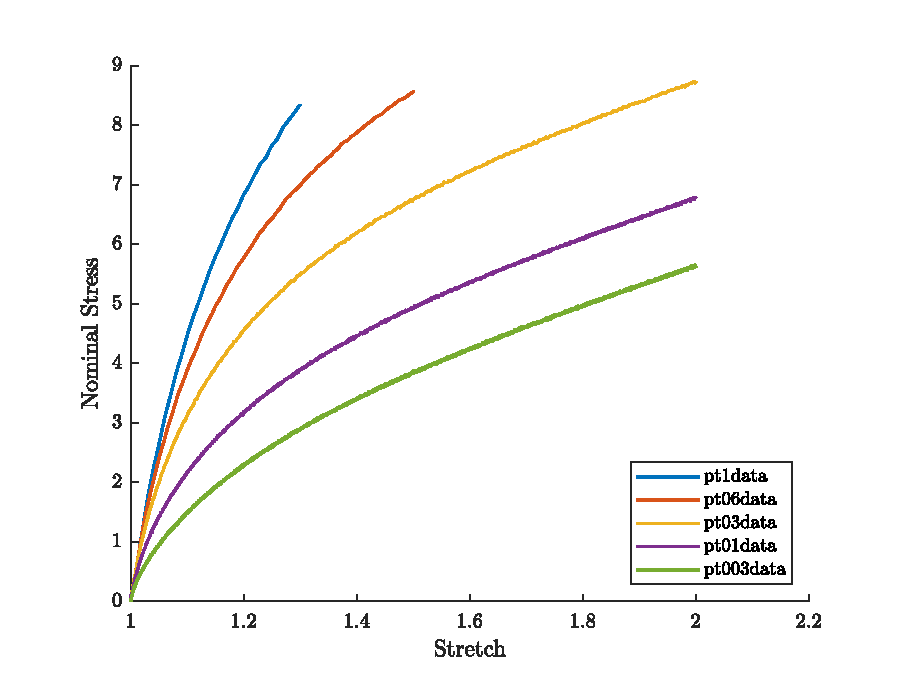
\includegraphics[width=0.85\textwidth]{ExperimentalData}
    \caption[Experimental data for a hydrogel]{Uniaxial tension experimental data of a hydrogel.}%
    \label{fig:uniaxial_experiments}
\end{figure}

\section{Non-Linear Least-Squares Optimization}
The goal of the parameter identification procedure is to find the set of paramaters for which the error between the experimental data and simulation is minimized. This then reduces to a non-linear least-squares optimization problem, in which a cost function is minimized over a set of variables (material parameters). Here, the cost function is given by 
\begin{equation}
    \text{Cost}({\hat{\bm{x}}_p}) = \sum_{j=1}^{E} \sum_{i=1}^{N} \big|\big|(\mathbf{P}{|}_{\text{exp}})^{j}_{i} - (\mathbf{P}{|}_{\text{sim}})^{j}_{i} \big|\big|
\end{equation}
where \(\mathbf{P}\) is the first Piola-Kirchoff stress tensor \cref{eq:def_firstpiolakirchoffstress} representing the nominal stress, \(E\) is the total number of experiments, \(N\) is the number of data points within an experiment, and \(||\bullet||\) is the Frobenius norm. In the case of uniaxial tension this reduces to 
\begin{equation}
    \text{Cost}({\hat{\bm{x}}_p}) = \sum_{j=1}^{E} \sum_{i=1}^{N} \,\big|\big|\,(\mathrm{P_{11}}{|}_{\text{exp}})^{j}_{i} - (\mathrm{P}_{11}{|}_{\text{sim}})^{j}_{i}\,\big|\big|
\end{equation}
The optimization problem can be then written as
\begin{equation}
   \underset{{\hat{\bm{x}}_p}}{\text{argmin }} \text{Cost}({\hat{\bm{x}}_p})
   \label{eq:constrained_optimization_cost}
\end{equation}
additionally, subject to constraints 
\begin{equation}
    \K> 0 \quad \text{ and } \quad (\km)^{k} > 0
    \label{eq:constraint_1}
\end{equation}
\begin{equation*}
    \mathrm{sgn}(\mu) = \text{sgn}(\alpha)  \quad \text{ and } \quad \mathrm{sgn}(\mum)^{k} = \text{sgn}(\am)^{k}
\end{equation*}
or 
\begin{equation}
\mu \alpha > 0 \quad \text{ and } \quad (\mum)^{k}(\am)^{k} > 0
\label{eq:constraint_2}
\end{equation}
since the bulk and shear modulus cannot have a negative value. In general, \cref{eq:constraint_1}  and \cref{eq:constraint_2} represent inequality constraints. Furthermore keeping \cref{eq:nd_rtime} and \cref{eq:nv_rtime} in mind, if the parameter vector specified in \cref{eq:parameters} would have been used, an additional equality constraint given by 
\begin{equation}
    \frac{\nd}{\mum \am} = \frac{\nv}{\km}
\end{equation}
would have to be satisfied. However, since the parameter vector specified in \cref{eq:parameters_red} is used, this constraint is already satisfied and need not be considered.

Solving a constrained optimization problem is much more resource intensive and time consuming as compared to solving an unconstrained optimization problem. Hence, the constrained optimization problem at hand \cref{eq:constrained_optimization_cost}, was converted into an unconstrained problem using the penalty method. To this end, a large penalty value is added to the cost when any of the constraints in \cref{eq:constraint_1}, \cref{eq:constraint_2} are violated. With this conversion, the optimization problem was given by 
\begin{equation*}
    \underset{{\hat{\bm{x}}_p}}{\text{argmin }} \text{Cost}({\hat{\bm{x}}_p})
\end{equation*}
\begin{equation}
    \text{Cost}({\hat{\bm{x}}_p}) = \sum_{j=1}^{E} \sum_{i=1}^{N} \,||\,(\mathrm{P_{11}}{|}_{\text{exp}})^{j}_{i} - (\mathrm{P}_{11}{|}_{\text{sim}})^{j}_{i}\,|| + \text{Penalty}({\hat{\bm{x}}_p})
    \label{eq:unconstrained_optimization}
\end{equation}

To solve this, the \texttt{lsqnonlin} function in MATLAB was used. For the cost function, the material response  was simulated for a given set of parameters \({\hat{\bm{x}}_p}\) using the twin implementation of the material model described in \cref{sec:twin_model}. Here, the first Piola-Kirchoff stress tensor can be found using \cref{eq:secondpiolakirchoff_stress}. As is needed by the material model, the deformation gradient \(\Ftot{}\) at the start (\texttt{DFGRD0}) and end (\texttt{DFGRD1}) of the current increment step were computed from stretch at the start \(\prstretche{}{t_{n-1}}\) and end \(\prstretche{}{t_{n}}\) of the current increment step, respectively from the experimental data. Furthermore, the time increment \(\Delta t\) was computed by taking the difference in time at the start and end of the current increment step. For the case of uniaxial tension, we have the deformation gradient at the end of the current time increment 
\begin{equation}
    (\Ftot)_{t_{n}} = 
    \begin{bmatrix}
    \prstretche{}{1} & 0 & 0 \\
    0 & \prstretche{}{2} & 0\\
    0 & 0 & \prstretche{}{3}
    \end{bmatrix} \evec{i} \otimes \evec{j}
\end{equation}
where \(\prstretche{}{1} = \prstretche{}{t_{n}}\) is the stretch in the axial direction and \(\prstretche{}{2} = \prstretche{}{3} = f({\prstretche{}{1}})\) are the stretches in the transverse directions. The deformation gradient \((\Ftot)_{t_{n-1}}\) at the start of the time increment can be found in a similar manner.

Initially during the optimization process, the material was considered to be perfectly incompressible, i.e. \(J=\text{det}(\Ftot{})=1\). Thus, the stretches in the transverse directions were given by, 
\begin{equation}
    \prstretche{}{2} = \prstretche{}{3} = \frac{1}{\sqrt{\prstretche{}{1}}}
\end{equation}
However, consequently the optimization problem was found to be insensitive to the bulk modulus \(\K\) and \((\km)^{k}\) as will be seen in \cref{sec:optimizataion_results}. Indeed if \(J=1\), keeping \cref{eq:principal_kirchoff_stress_eq_vol}, \cref{eq:principal_kirchoff_stress_vol} in mind, there is no contribution of volumetric stress to the total stress, and hence, \(\K\) and \((\km)^{k}\) could take any value without affecting the simulated response. Furthemore, as a result, the nominal stress in the tranvese directions \(\mathrm{P}_{22}{|}_{\text{sim}} = \mathrm{P}_{33}{|}_{\text{sim}} \neq 0\). This negates the fact that, for a uniaxial tension experiment stresses in the transverse direction are zero. 

Later on, to avoid these shortcomings, given the stretch in the axial direction \(\lambda_1\), the stretches in the tranverse directions \(\lambda_2\) and \(\lambda_3\) were computed by finding the roots of the function
\begin{equation}
    \mathrm{P}_{22}{|}_{\text{sim}}(\lambda_1, \lambda_2, \lambda_3) = 0 \text{ or } \mathrm{P}_{33}{|}_{\text{sim}} (\lambda_1, \lambda_2, \lambda_3) = 0
    \label{eq:optimization_NR}
\end{equation}
For this, the root-finding function \texttt{fsolve} from MATLAB, which employs a Newton-Raphson's method, was used. Here, again the first Piola-Kirchoff stress tensor was calculated using the twin implementation of the material model described in section \cref{sec:twin_model}.

\section{Results of the Optimization Problem}
\label{sec:optimizataion_results}
Firstly, considering the viscoelastic material model with a single relaxation mechanism \((k=1)\), when the cost was calculated including data from all the five experiments, it was not possible to find a suitable set of material parameters to fit the simulated response to the experimental data. However, for certain cases, when only a single experiment was considered to calculate the cost, it was possible to find a set of material parameters that would fit the material model response to the selected experiment. On the other hand, when these set of parameters were used to simulate the other experiments, the material response was not in agreement with the experimental data. This indicated that the viscoelastic material model with a single relaxation mechanism was too simple to sufficiently characterize the hydrogel considered. 

\begin{figure}[htpb]
    \centering
    \subfloat[]{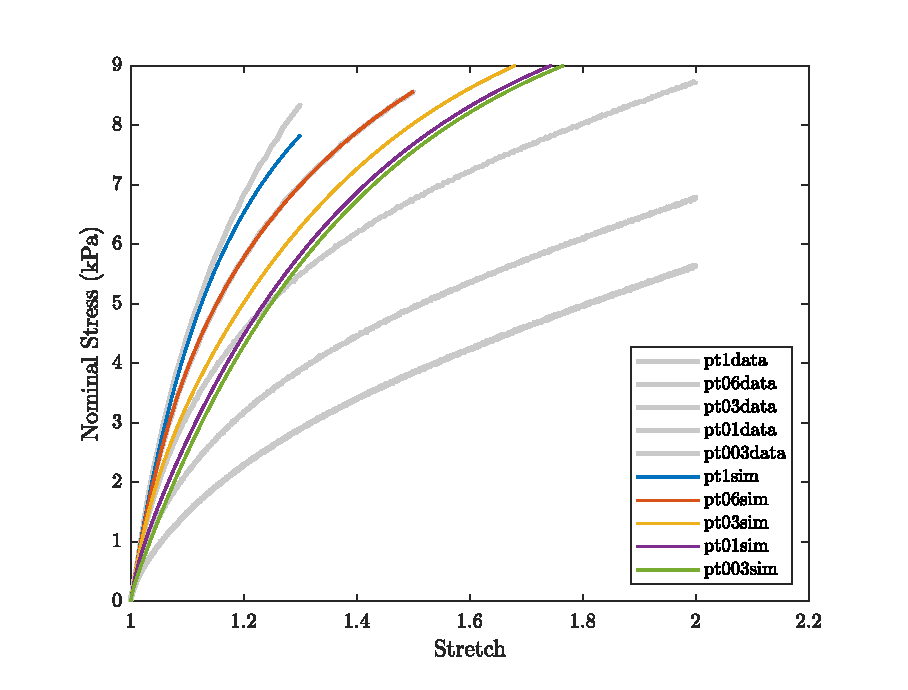
\includegraphics[width = 0.85\textwidth]{Optimization_pt06}} \label{fig:parameter_optimization_1EL_pt06} 
    \subfloat[]{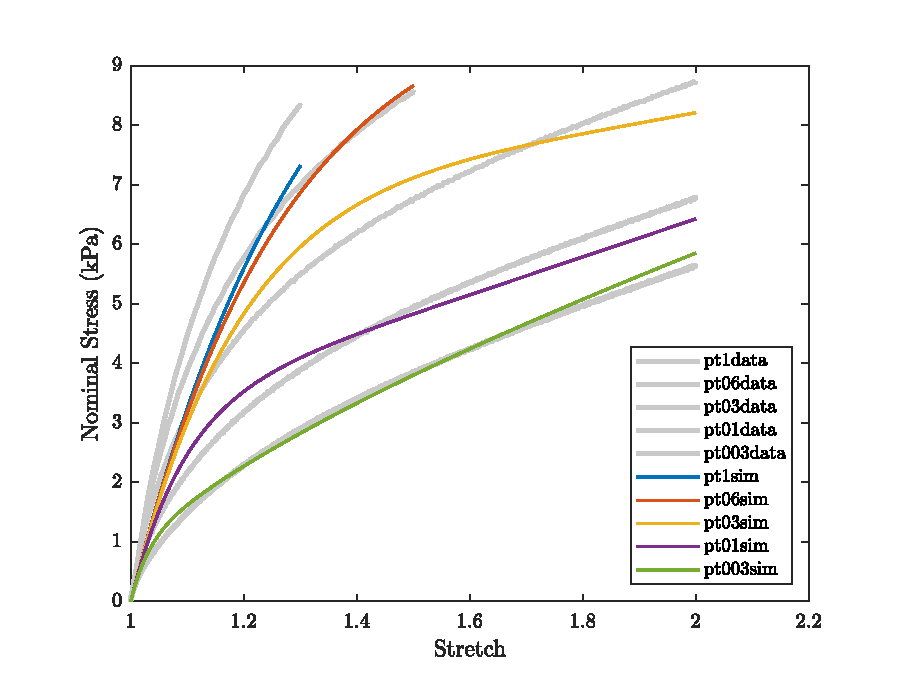
\includegraphics[width = 0.85\textwidth]{Optimization1EL_NR_all}} \label{fig:parameter_optimization_1EL_all}\\
    \caption[Parameter identification 1]{Parameter identification of viscoelastic material model with one relaxation mechanisms \((k=1)\) fit to (a) the experiment with stretch rate \(0.06s^{-1}\) and (b) all the five experiments together}
    \label{fig:parameter_optimization_1EL}
\end{figure}

Next, the viscoelastic material models with two \((k=2)\) or three \((k=3)\) relaxation mechanisms were considered. Even though, it was computationally more expensive to solve the optimization problem \cref{eq:constrained_optimization_cost}, it was possible to find a set of suitable parameters that would fit the material response to all the experiments together. As can be seen in \cref{fig:parameter_optimization} the response from the model with three relaxation mechanisms \((k=3)\) fits better to the experimental data. However, since certain material model parameters have no physical meaning when considered individually, the optimization problem provided different solutions when different starting points \((\bm{x}_{p})_{0}\) in the parameter space were considered. Moreover, as can be seen from  optimized parameter sets (a) and (b) in \cref{tab:opt_param_sets}, it was found that the bulk  \(\K{}, \km^{1}, \km^{2}\) for the elastic and inealstic parts in the model with two relaxation mechanisms (2EL) had little to no effect on the parameter optimization procedure. 


\begin{figure}[htpb]
    \centering
    \subfloat[]{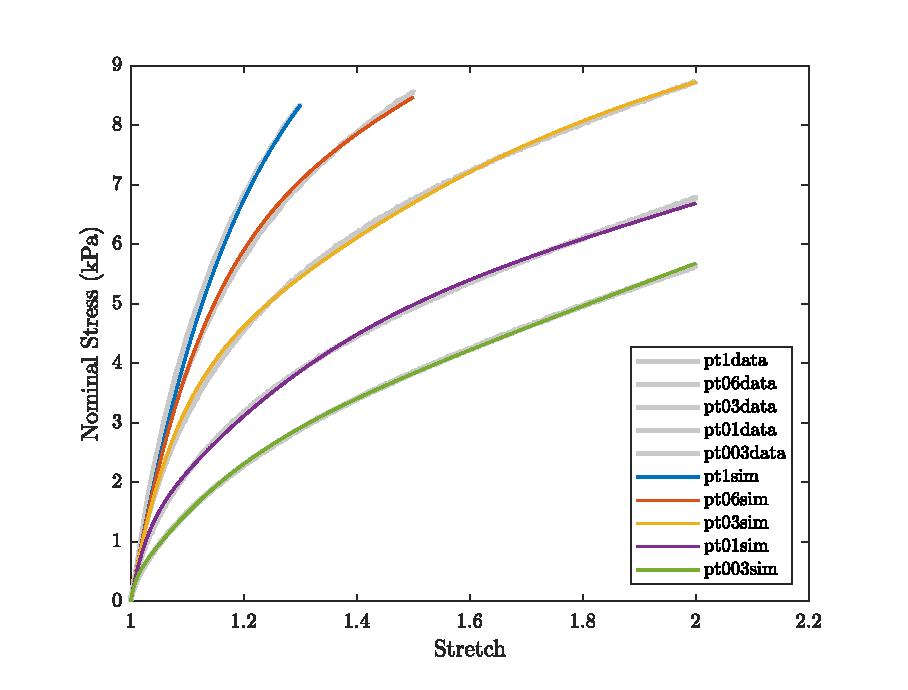
\includegraphics[width = 0.85\textwidth]{Optimization2EL_all}} \label{fig:parameter_optimization_2EL} 
    \subfloat[]{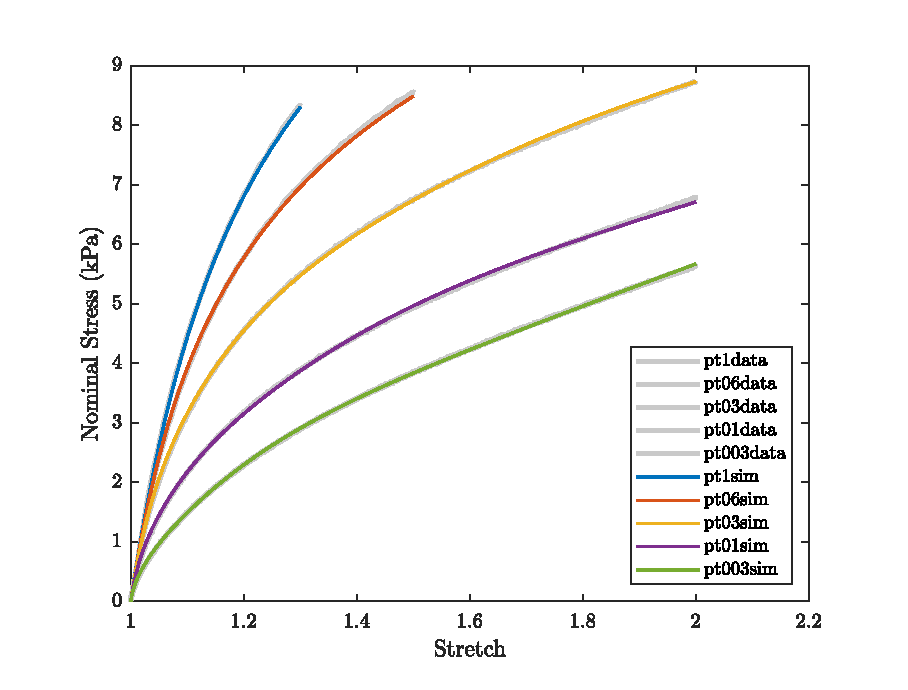
\includegraphics[width = 0.85\textwidth]{Optimization3EL_all}} \label{fig:parameter_optimization_3EL}\\
    \caption[Parameter identification 2]{Parameter identification of viscoelastic material model (a) with two relaxation mechanisms \((k=2)\) and (b) with three relaxation mechanisms \((k=3)\) considering \(J=1\) and \(\lambda_{2,3} = \frac{1}{\sqrt{\lambda_1}}\)}
    \label{fig:parameter_optimization}
\end{figure}

\begin{figure}[htpb]
    \centering
    \subfloat[]{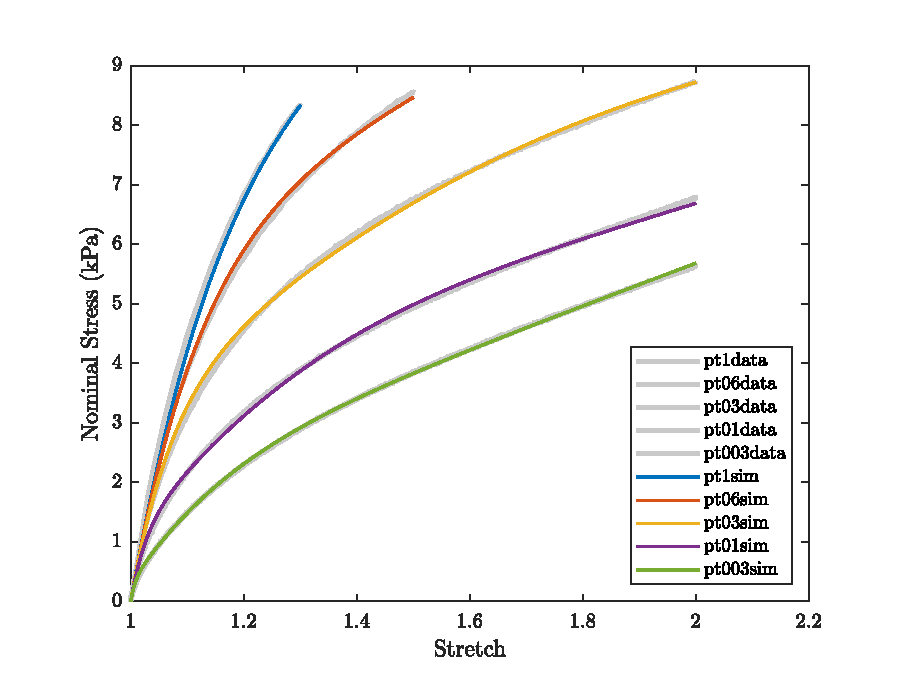
\includegraphics[width = 0.85\textwidth]{Optimization2EL_NR_all.eps}} \label{fig:parameter_optimization_nr_2EL} 
    \subfloat[]{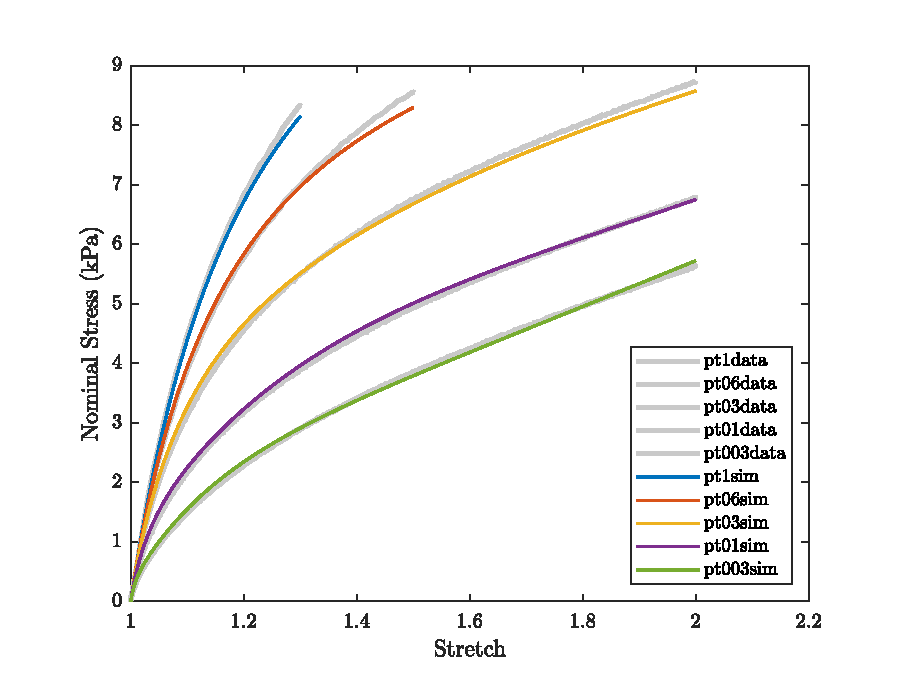
\includegraphics[width = 0.85\textwidth]{Optimization3EL_NR_all.eps}} \label{fig:parameter_optimization_nr_3EL}\\
    \caption[Parameter identification 3]{Parameter identification of viscoelastic material model (a) with two relaxation mechanisms \((k=2)\) and (b) with three relaxation mechanisms \((k=3)\) satisfying the condition \(\mathrm{P}_{22,33} = 0\)}
    \label{fig:parameter_optimization_nr}
\end{figure}


\begin{figure}[htbp]
    \centering
    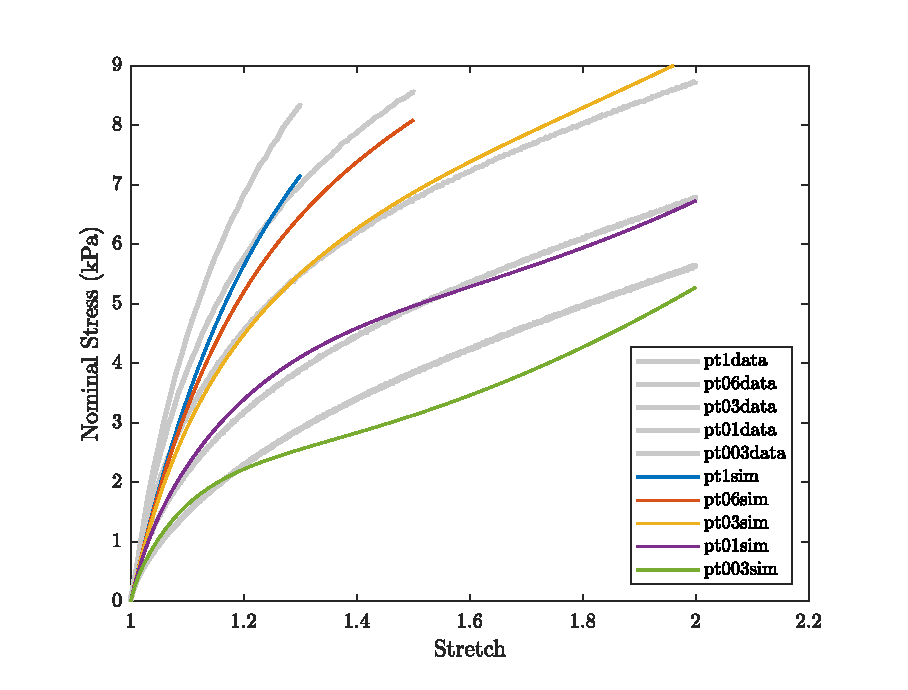
\includegraphics[width=0.85\textwidth]{Optimization2EL_NRred_all.eps}
    \caption[Parameter identification 4]{Parameter identification for a viscoelastic material model with two relaxation mechanisms \((k=2)\) and a reduced parameter set}%
    \label{fig:parameter_optimization_red}
\end{figure}

Furthermore, the cost function was updated such that the stresses in the transverse direction would be zero in order to exactly mimic the uniaxial tension experiment. It must be noted that, the root-finding procedure (Newton-Raphson's method), that was necessary to achieve this condition, led to a tremendous increase in the number of computations performed within the cost function. Nevertheless, using this revised cost function, it was possible find a set of suitable parameters for the models with two \((k=2)\) and three \((k=3)\) relaxation mechanisms that simulated a response which was in close agreement to experimental data. Here, the response of the model with two relaxation mechanisms \((k=2)\) fit the experimental data better as can be seen in \cref{fig:parameter_optimization_nr}. For the model with one relaxation mechanism \((k=1)\), however, even after the cost function update, it was still not possible to find a set of parameters to fit the simulation response to all the experiments together. 

Finally, in an attempt to further reduce the number of model parameters, the viscous parameters \((\mum)^{k}, (\am{})^{k}, (\km{})^{k}\) were chosen to be equal to elastic parameters \(\mu, \alpha, \K\) respectively, as is sometimes done in literature \cite[][see Sec. 5]{Reese1998Sep}. For the model with two relaxation mechanisms\((k=2)\), using this methodology was found to be ineffective. Again as can be seen in \cref{fig:parameter_optimization_red}, the model rendered itself to be very simple to characterize the uniaxial tension experiments of the hydrogel. The sets of optimized parameters for all the optimization procedures carried out are summarized in \cref{tab:opt_param_sets}.

 


{\renewcommand{\arraystretch}{1.5}%
\begin{table}[htbp]
    \centering
    \begin{tabular}{cS[table-format=5.4]S[table-format=5.4]S[table-format=5.4]S[table-format=5.4]S[table-format=5.4]}
        \toprule
           &  {\text{2EL\({}_{1}\)}} &  {\text{2EL\({}_{2}\)}} &  {\text{2EL\({}_{\text{NR}}\)}} &  {\text{3EL}} &  {\text{3EL\({}_{\text{NR}}\)}} \\ \midrule   
        \(\bm{x}_{p}\)    &  {\text{(a)}} &  {\text{(b)}} &  {\text{(c)}} &  {\text{(d)}} &  {\text{(e)}} \\ \midrule   
        \(\mu\)           &  0.0040       &     0.0040    & 0.0026        &     0.0039    &     0.0024	  \\
        \(\alpha\)        &  2.1471       &     2.1474    & 2.1478        &     2.1578    &     2.2817	  \\ 
        \(\K\)            &  4.0000       &     40.0000   & 29.4615       &     40.0000   &     5.2712	  \\
        \(\mum^{1}\)      &  0.0686       &     0.0664    & 0.0643        &     0.0414    &     0.1182	  \\
        \(\am^{1}\)       &  0.5827       &     0.6011    & 0.4168        &     0.8837    &     0.1168	  \\
        \(\km^{1}\)       &  6.0000       &     60.0000   & 61.3862       &     59.9990   &     25.7008   \\
        \(\tau_{r}^{1}\)  &  3158.0       &     1.3159    & 1.2985        &     0.4912    &     0.3146	  \\
        \(\mum^{2}\)      &  0.0017       &     0.0017    & 0.0011        &     0.0042    &     0.1340	  \\
        \(\am^{2}\)       &  3.5330       &     3.5302    & 3.5251        &     3.5012    &     0.1376	  \\ 
        \(\km^{2}\)       &  5.0000       &     25.0000   & 29.0539       &     60.0006   &     14.4123   \\ 
        \(\tau_{r}^{2}\)  & 36.9815       &     36.9446   & 36.5179       &     3.3429    &     1.5602	  \\ 
        \(\mum^{3}\)      &     \text{-}  &     \text{-}  &    \text{-}   &     0.0014    &     0.0032	  \\
        \(\am^{3}\)       &     \text{-}  &     \text{-}  &    \text{-}   &     3.4523    &     1.7457	  \\ 
        \(\km^{3}\)       &     \text{-}  &     \text{-}  &    \text{-}   &     24.9999   &     2.7381	  \\ 
        \(\tau_{r}^{3}\)  &     \text{-}  &     \text{-}  &    \text{-}   &     45.9230   &     26.4516   \\ 
        \bottomrule
    \end{tabular}
    \caption[Optimized parameter sets]{Optimized parameter sets for the viscoealstic material model for the dual cross-link self-healing hydrogel.
    \newline \((k)\)EL stands for a model with \(k\) relaxation mechanisms \newline \((\bullet)_{\text{NR}}\) stands for models using cost function with the modified root-finding (Newton-Raphson's) procedure \cref{eq:optimization_NR}}
    \label{tab:opt_param_sets}
\end{table}}




\chapter{Numerical Simulations}%
\label{chapter:five}
In order to test the implemented \texttt{UMAT} subroutines  for the viscoelastic material model, numerical simulations were carried out in ABAQUS. To this end, finite element models with both a single element and multiple elements were considered. Here, material parameters identified in \cref{tab:opt_param_sets} for the dual cross-link self-healing hydrogel material were used.

\section{Single-Element Simulations}
Using a model with a single finite element, it is possible to test the developed \texttt{UMAT} and check for any implementation errors. For this, a uniaxial tension test mimicing the experimental data in \cref{fig:uniaxial_experiments} was simulated using one C3D8H\footnote[1]{8-noded 3D continuum element with hybrid formulation in ABAQUS} element of size 10mm x 10mm x 10mm.

Firstly, the element was fixed \((u_{x}, u_{y}, u_{z} = 0)\) on one end \((x=0)\) and a ramp displacement of 10mm was applied in the x-direction with a constant displacement rate on the other end \((x=10)\). The constant displacement rate 
\begin{equation}
    \dot{u}_{x} = \mathrm{L}_{0} \dot{\lambda_{x}}
    \label{eq:displacement_rate}
\end{equation}
was derived from the stretch rate given the fact that
\begin{equation}
     \lambda_{x} = 1 + \dfrac{{u_{x}|}_{x=10}}{\mathrm{L}_{0}}
\end{equation}  where \(L_{0} = 10\). 
In order to compare the results with the experimental data and the twin implementation in MATLAB, the simulations were carried out for stretch rates ranging from \(0.1s^{-1}\) to \(0.003s^{-1}\). Furthermore, the implemented viscoelastic material models with, both, two \((k=2)\) and three \((k=3)\) relaxation mechanisms were used. It was found that, the response of the material model was affected by the stretch rates as seen in \cref{fig:abaqus_comparison}, which was as expected. However, for both the models (2EL and 3EL), the material response was not in agreement with the experimental data. The reason for this contradiction could either be the fact that, ABAQUS implements logarithmic strains for problems with large deformation, or, that the finite element formulation used in ABAQUS differs from the purely analytical approach that was used to calculate the material response in MATLAB during the parameter identification procedure. It is also possible that experimental data from multiple loading cases is required for identifying the optimal set of parameters\cite{Kleuter2007Jul}. Nevertheless, this needs further investigation. One possible way to avoid this deviation would be to use ABAQUS to calculate the material response instead of MATLAB for the cost function in \cref{eq:unconstrained_optimization}. This, however, is also not dealt with in this work.

\begin{figure}[htpb]
    \centering
    \subfloat[]{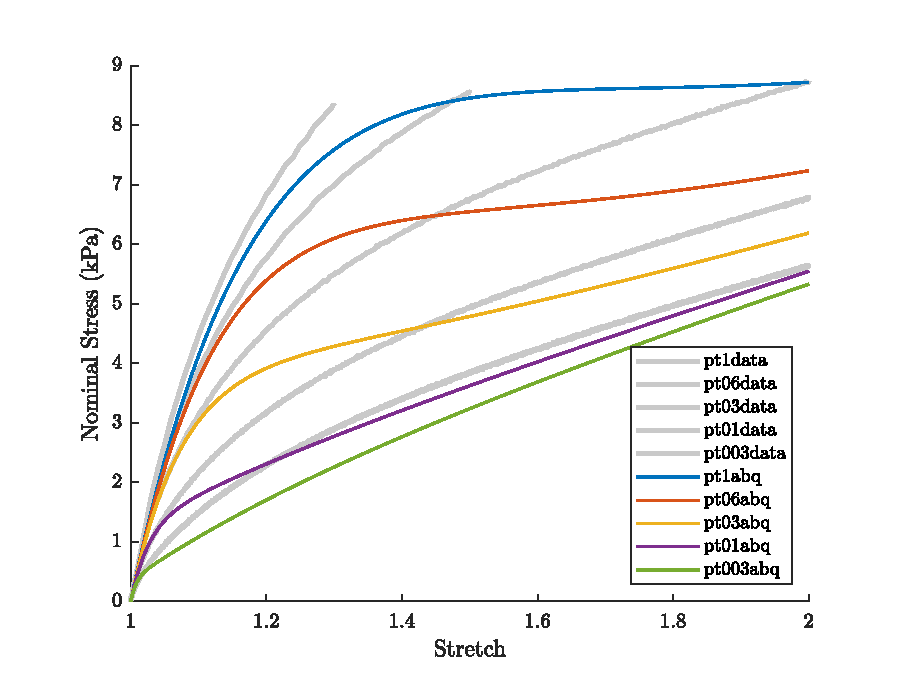
\includegraphics[width = 0.85\textwidth]{2EL_Abaqus_NR.eps}} \label{fig:abaqus_comparison_2EL}
    \subfloat[]{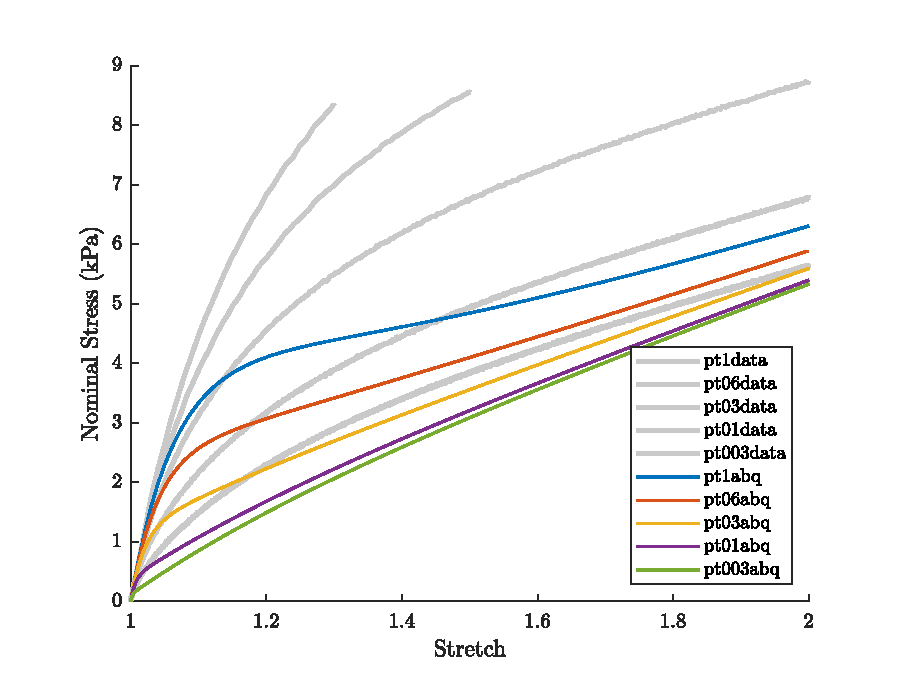
\includegraphics[width = 0.85\textwidth]{3EL_Abaqus_NR.eps}} \label{fig:abaqus_comparison_3EL}\\
    \caption[Uniaxial tension test simulation]{Uniaxial tension test simulation in ABAQUS using viscoelastic material model (a) with two relaxation mechanisms \((k=2)\) and (b) with three relaxation mechanisms \((k=3)\) and respective material parameters \(\bm{x}_{p}\) for \(2\mathrm{EL}_{\mathrm{NR}}\), \(3\mathrm{EL}_{\mathrm{NR}}\) taken from \cref{tab:opt_param_sets}}
    \label{fig:abaqus_comparison}
\end{figure}

Next, the single element model was subjected to uniaxial loading followed by unloading. In this case, the element was fixed \((u_{x}, u_{y}, u_{z} = 0)\) on one end \((x=0)\).  On the other end \((x=10)\) a ramp displacement of 10mm followed by a negative ramp displacement of 10mm was applied in the x-direction with a constant displacement rate  given by \cref{eq:displacement_rate}. Here, again the simulations were carried out for stretch rates varying from \(0.1s^{-1}\) to \(0.003s^{-1}\). For this simulation, only the viscoelastic material model with two relaxation mechanisms \((k=2)\) was used. The material response for the simulations is given in \cref{fig:loading_unloading_abaqus}. Here, it can be seen that the material response is generally affected by the stretch rates. Furthermore, during unloading, the nominal stress \(\mathrm{P}_{11} = 0\) for stretch \(\prstretche{}{1} > 1\). This effect is desired and is also in agreement with the  material model developed by \citeauthor{Long2014Oct} \cite{Long2014Oct} for the hydrogel material at hand.

\begin{figure}[htbp]
    \centering
    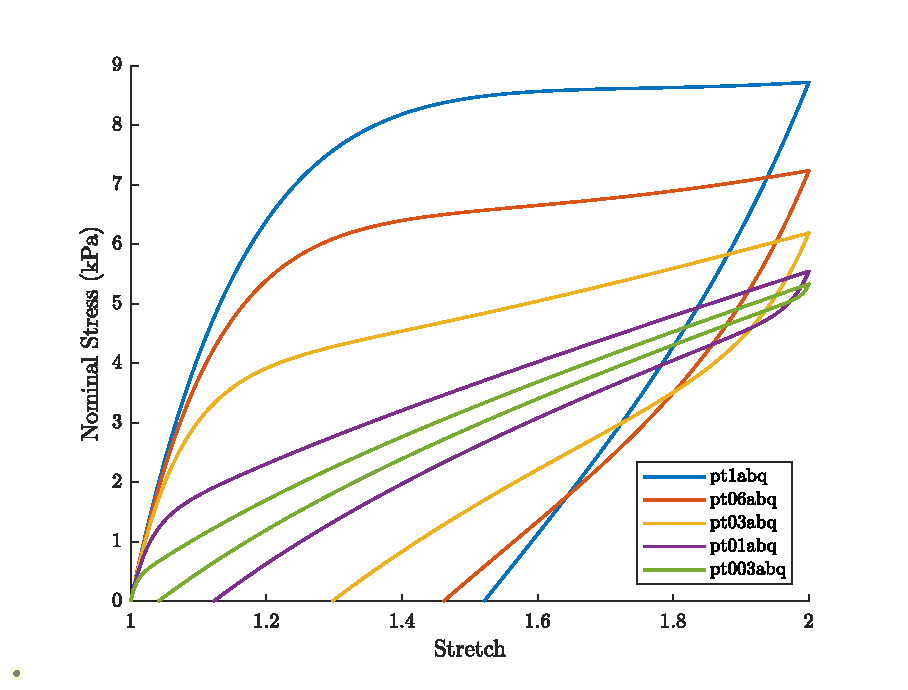
\includegraphics[width=0.95\textwidth]{2EL_loading_unloading_Abaqus.eps}
    \caption[Uniaxial loading and unloading simulation]{Uniaxial loading-unloading simulation in ABAQUS for viscoelastic material model with two relaxation mechanisms \((k=2)\) using material parameters \(\bm{x}_{p}\) for \(2\mathrm{EL}_{\mathrm{NR}}\) (\cref{tab:opt_param_sets}) }%
    \label{fig:loading_unloading_abaqus}
\end{figure}

Finally, the single element model was subjected to uniaxial loading and relaxation. Here, again the element was fixed \((u_{x}, u_{y}, u_{z} = 0)\) on one end \((x=0)\). On the other end \((x=10)\), a ramp displacement of 10mm was applied in the x-direction with a constant displacement rate given by \cref{eq:displacement_rate}. At the end of this step, the displacement was held constant at 10mm and the material was allowed to relax. For this simulation too, only the implemented viscoelastic material model with two relaxation mechanisms \((k=2)\) was used. The material response for the simulations is given in \cref{fig:loading_relaxation_abaqus}. Here during the relaxation phase, it can be seen that after certain time, the stress \(\sigmatot\), and hence, \(\mathbf{P}\) within the element reduces to the equillibrium stress \(\sigmaeq\), and hence \(\mathbf{P}_{\mathrm{EQ}}\), which is expected behaviour for a viscoelastic material model. 

\begin{figure}[htbp]
    \centering
    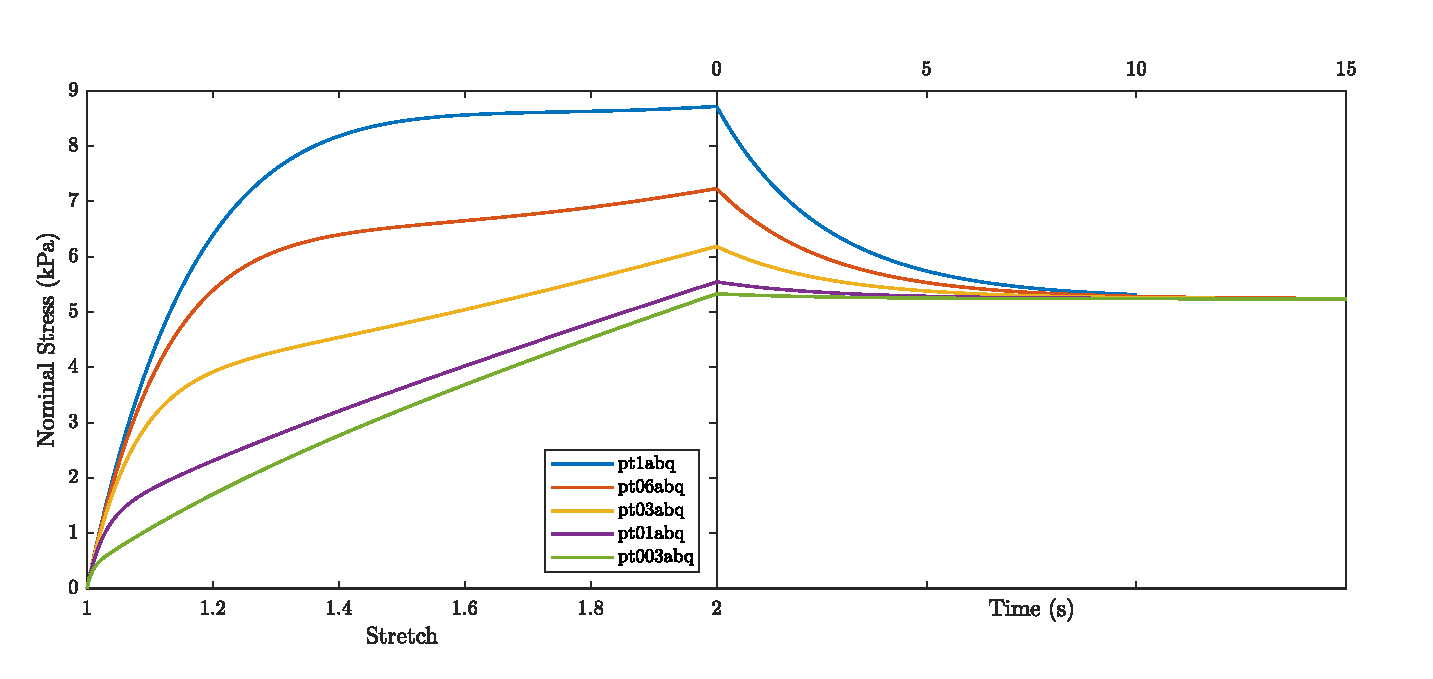
\includegraphics[width=1\textwidth]{2EL_loading_relaxation_Abaqus.eps}
    \caption[Uniaxial loading and relaxation simulation]{Uniaxial loading-relaxation simulation for viscoelastic material model in ABAQUS  with two relaxation mechanisms \((k=2)\) using material parameters \(\bm{x}_{p}\) for \(2\mathrm{EL}_{\mathrm{NR}}\) (\cref{tab:opt_param_sets})}%
    \label{fig:loading_relaxation_abaqus}
\end{figure}

\section{Multi-Element Simulations}
Now that the implemented viscoelastic material models demonstrated the expected behaviour in finite element models involving a single element, they were further tested with finite element models involving multiple elements. To this end, a column twisting simulation with a pressure-follower load as described in \cref{fig:twister} was employed\cite{Bonet2015Jan}. The column was 6mm tall and had a cross section of 1mm~x~1mm. An additional section of 3mm~x~1mm~x~1mm on the top was used to apply the pressure-follower load. The response of the model was then observed at the point \(A \equiv (1.0, 0.0, 6.5)\). The geometry was discretized with a mesh size of 0.25mm or 0.1mm resulting in 576 and 9000 elements respectively. Furthermore, both C3D8H and C3D20H\footnote[1]{20-noded 3D continuum element with hybrid formulation in ABAQUS} element formulations were employed.

\begin{figure}[htbp]
    \centering
    \includegraphics[width=0.9\textwidth]{twister_} 
    \caption[Column twisting simulation]{Column twisting simulation model definition using pressure-follower load (left) and exemplary deformed shape (right)}%
    \label{fig:twister}
\end{figure}

The response of the column twisting simulations is as shown in \cref{fig:column_twisting}. In the case of \emph{slow} simulations, the pressure was ramped at a rate of 2.5~kPa/s and 1.5~kPa/s for simulations with C3D8H and C3D20H elements respectively. For all other simulations, the pressure was ramped at a rate of 1~MPa/s. It is evident from the results that the invariants of the Cauchy stress tensor \(I_{\sigmatot}, II_{\sigmatot}, III_{\sigmatot} \text{ and } II_{\mathrm{dev}(\sigmatot)}\) are affected by the rate of deformation or  the rate of pressure application. The stress invariants for simulations with slower pressure application rate were always lower. This is because at slower rates of deformation or pressure application, the contribution of the non-equillibrium stress \(\sigmaneq\) to the total stress \(\sigmatot\) is lower, which is also the expected behaviour.

\begin{figure}[htpb]
    \centering
    \subfloat[]{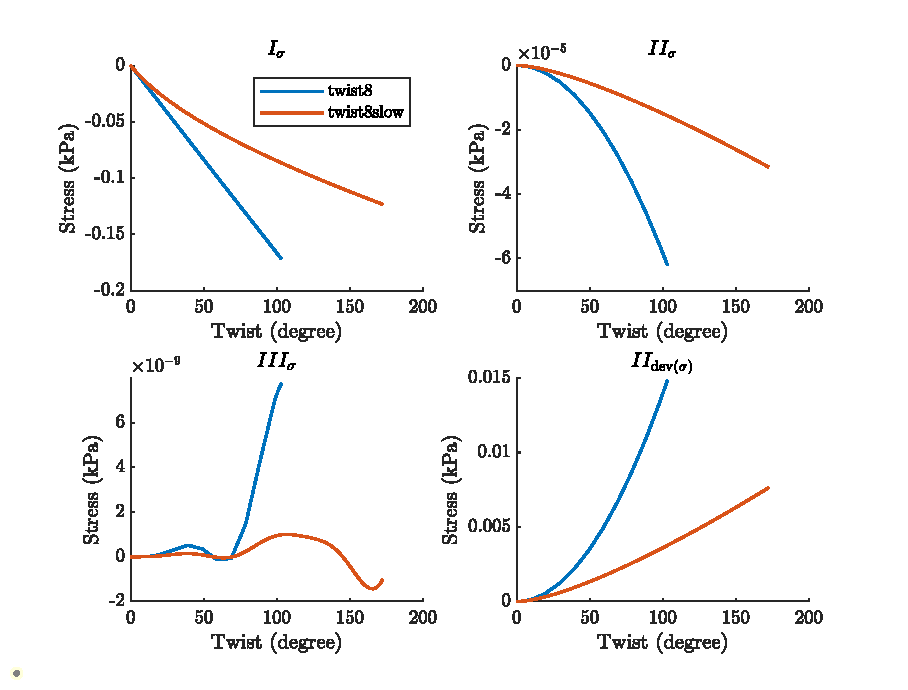
\includegraphics[width = 0.95\textwidth]{2EL_column_twist8.eps}} \label{fig:twist8} 
    \subfloat[]{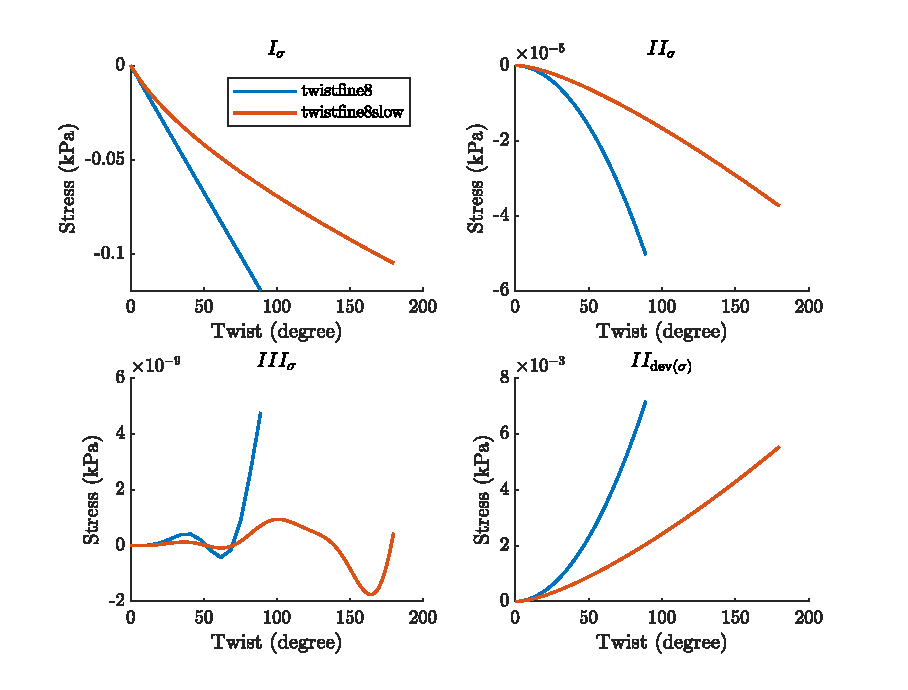
\includegraphics[width = 0.95\textwidth]{2EL_column_twistfine8.eps}} \label{fig:twistfine8}
\end{figure}
\begin{figure}[htpb]\ContinuedFloat
    \centering
    \subfloat[]{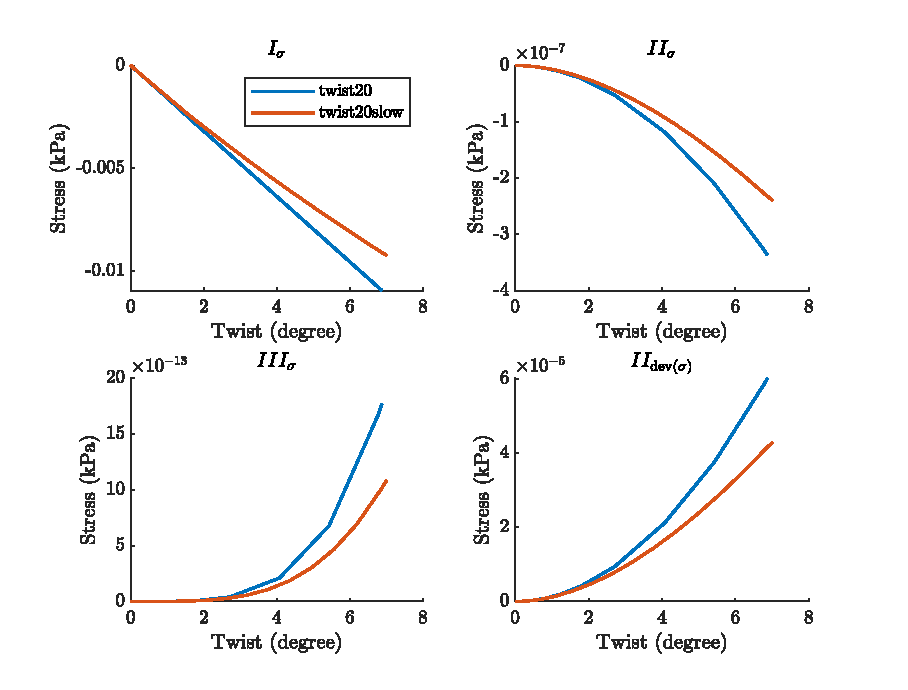
\includegraphics[width = 0.95\textwidth]{2EL_column_twist20.eps}} \label{fig:twist20}
    \caption[Column twisting simulation results]{Column twisting simulation results in ABAQUS discretized with (a) 576 C3D8H, (b) 9000 C3D8H and (c) 576 C3D20H elements using viscoelastic material model with two relaxation mechanisms \((k=2)\) and material parameters \(\bm{x}_{p}\) for \(2\mathrm{EL}_{\mathrm{NR}}\) (\cref{tab:opt_param_sets})}\label{fig:column_twisting}
\end{figure}





\chapter{Conclusion}
Hydrogels are being increasingly used in biomedical applications. It has therefore become important to understand their characteristics. In order to understand the suitability of hydrogels to a specific application, it is convenient to be able to regenerate the material response in a simulation with the help of a material model. Various mathematical models have been developed over the years to describe the characteristics of hydrogels. However, these have been based on the underlying physical and chemical phenomena. Since, hydrogels also exhibit viscoelastic properties, it was sought to characterize the the hydrogels using the finite viscoelasticity theory in this work. For this, user material (\texttt{UMAT}) subroutines for finite viscoelasticity theory using the Ogden class of strain energy functions with one, two and three relaxation mechanisms were implemented. The necessary theory required to implement the material model as well as the preliminary theory of continuum mechanics was briefly summarized. Furthermore, the step-by-step implementation details for the \texttt{UMAT} were also explained. 

Thereafter, so that the implemented material model could characterize a hydrogel material, parameter identification was carried out using a non-linear least square optimization procedure along with a twin implementation of the \texttt{UMAT} in MATLAB. Here it was found that, the \texttt{UMAT} with a single relaxation mechanism was not able to replicate the material response of the hydrogel material from the experimental data. Additionally, although the optimal set parameters for \texttt{UMAT}s with two and three relaxation mechanisms were identified, it was found later on, that the models with these parameters generated a material response in ABAQUS simulations which disagreed with the experimental data. However, this does not altogether disregard the use of the finite viscoelasticity theory to characterize hydrogel materials, but suggests towards finding another approach for the parameter identification procedure. For future work in this regard, as an alternate, it could be possible to use the material response from the finite element simulation in ABAQUS for calculation of the cost function in the optimization procedure. Also, for material models that employ Ogden class of strain energy functions, it is recommended to perform the parameter identification procedure using experimental data from additional load cases, viz. biaxial tension and pure shear. Lastly, as an improvement, the \texttt{UMAT} could also be optimized to reduce the number of memory allocations for local variables in the models with two or more relaxation mechanisms to make the subroutine faster and efficient.




% 
\clearpage{} \addcontentsline{toc}{chapter}{Bibliography}
{\raggedright%
\printbibliography{}%
}
\clearpage{}

\pagenumbering{Roman}
\appendix
\chapter{\texttt{UMAT} Source Code}%
\label{appendixA}
Below is the source code implementation of the viscoelastic material model with two relaxation mechanisms (viscous elements). Here, the steps described in \cref{sec:implementation_algorithm} are followed, which is evident from the comments in the source.
\lstinputlisting[language=Fortran]{chapters/VISC_OGDEN_2EL.for}

\end{document}